
%% bare_conf.tex
%% V1.3
%% 2007/01/11
%% by Michael Shell
%% See:
%% http://www.michaelshell.org/
%% for current contact information.
%%
%% This is a skeleton file demonstrating the use of IEEEtran.cls
%% (requires IEEEtran.cls version 1.7 or later) with an IEEE conference paper.
%%
%% Support sites:
%% http://www.michaelshell.org/tex/ieeetran/
%% http://www.ctan.org/tex-archive/macros/latex/contrib/IEEEtran/
%% and
%% http://www.ieee.org/

%%*************************************************************************
%% Legal Notice:
%% This code is offered as-is without any warranty either expressed or
%% implied; without even the implied warranty of MERCHANTABILITY or
%% FITNESS FOR A PARTICULAR PURPOSE! 
%% User assumes all risk.
%% In no event shall IEEE or any contributor to this code be liable for
%% any damages or losses, including, but not limited to, incidental,
%% consequential, or any other damages, resulting from the use or misuse
%% of any information contained here.
%%
%% All comments are the opinions of their respective authors and are not
%% necessarily endorsed by the IEEE.
%%
%% This work is distributed under the LaTeX Project Public License (LPPL)
%% ( http://www.latex-project.org/ ) version 1.3, and may be freely used,
%% distributed and modified. A copy of the LPPL, version 1.3, is included
%% in the base LaTeX documentation of all distributions of LaTeX released
%% 2003/12/01 or later.
%% Retain all contribution notices and credits.
%% ** Modified files should be clearly indicated as such, including  **
%% ** renaming them and changing author support contact information. **
%%
%% File list of work: IEEEtran.cls, IEEEtran_HOWTO.pdf, bare_adv.tex,
%%                    bare_conf.tex, bare_jrnl.tex, bare_jrnl_compsoc.tex
%%*************************************************************************

% *** Authors should verify (and, if needed, correct) their LaTeX system  ***
% *** with the testflow diagnostic prior to trusting their LaTeX platform ***
% *** with production work. IEEE's font choices can trigger bugs that do  ***
% *** not appear when using other class files.                            ***
% The testflow support page is at:
% http://www.michaelshell.org/tex/testflow/



% Note that the a4paper option is mainly intended so that authors in
% countries using A4 can easily print to A4 and see how their papers will
% look in print - the typesetting of the document will not typically be
% affected with changes in paper size (but the bottom and side margins will).
% Use the testflow package mentioned above to verify correct handling of
% both paper sizes by the user's LaTeX system.
%
% Also note that the "draftcls" or "draftclsnofoot", not "draft", option
% should be used if it is desired that the figures are to be displayed in
% draft mode.
%
%\documentclass[10pt, conference, compsocconf]{IEEEtran}
\documentclass[10pt, conference]{IEEEtran}
% Add the compsocconf option for Computer Society conferences.
%
% If IEEEtran.cls has not been installed into the LaTeX system files,
% manually specify the path to it like:
% \documentclass[conference]{../sty/IEEEtran}




\usepackage{tikz}
\usetikzlibrary{shapes}
\usetikzlibrary{automata}

\usepackage[usenames,dvipsnames]{pstricks}
\usepackage{epsfig}
%\usepackage{pst-grad} % For gradients
%\usepackage{pst-plot} % For axes

\usepackage{palatino}
\RequirePackage{ifthen}
\usepackage{latexsym}
\RequirePackage{amsmath}
\RequirePackage{amsthm}
\RequirePackage{amssymb}
\RequirePackage{xspace}
\RequirePackage{graphics}
\usepackage{xcolor}
%\usepackage{fullpage}
\usepackage{schemabloc}
\RequirePackage{textcomp}
\usepackage{keyval}
%\usepackage{listings}
\usepackage{xspace}
\usepackage{mathrsfs}
%\usepackage{textcomp}
%\usepackage{graphicx}
\usepackage{paralist}
\usepackage{amsmath,amssymb,url,listings,mathrsfs}
%\usepackage{pvs}
%\usepackage{supertabular,alltt,latexsym}
%\usepackage{multicol,multirow,epsfig}
%\usepackage[dvips, usenames]{color}
\usepackage{framed}
\usepackage{lipsum}
%\usepackage[dvipsnames]{color}

\definecolor{reddish}{rgb}{1,.8,0.8}
\definecolor{blueish}{rgb}{0.8,.8,1}
\definecolor{greenish}{rgb}{.8,1,0.8}
\definecolor{yellowish}{rgb}{1,1,.20}


% Some very useful LaTeX packages include:
% (uncomment the ones you want to load)


% *** MISC UTILITY PACKAGES ***
%
%\usepackage{ifpdf}
% Heiko Oberdiek's ifpdf.sty is very useful if you need conditional
% compilation based on whether the output is pdf or dvi.
% usage:
% \ifpdf
%   % pdf code
% \else
%   % dvi code
% \fi
% The latest version of ifpdf.sty can be obtained from:
% http://www.ctan.org/tex-archive/macros/latex/contrib/oberdiek/
% Also, note that IEEEtran.cls V1.7 and later provides a builtin
% \ifCLASSINFOpdf conditional that works the same way.
% When switching from latex to pdflatex and vice-versa, the compiler may
% have to be run twice to clear warning/error messages.





% *** CITATION PACKAGES ***
%
%\usepackage{cite}
% cite.sty was written by Donald Arseneau
% V1.6 and later of IEEEtran pre-defines the format of the cite.sty package
% \cite{} output to follow that of IEEE. Loading the cite package will
% result in citation numbers being automatically sorted and properly
% "compressed/ranged". e.g., [1], [9], [2], [7], [5], [6] without using
% cite.sty will become [1], [2], [5]--[7], [9] using cite.sty. cite.sty's
% \cite will automatically add leading space, if needed. Use cite.sty's
% noadjust option (cite.sty V3.8 and later) if you want to turn this off.
% cite.sty is already installed on most LaTeX systems. Be sure and use
% version 4.0 (2003-05-27) and later if using hyperref.sty. cite.sty does
% not currently provide for hyperlinked citations.
% The latest version can be obtained at:
% http://www.ctan.org/tex-archive/macros/latex/contrib/cite/
% The documentation is contained in the cite.sty file itself.

\usepackage[pdftex]{hyperref}
\hypersetup{
  pdftitle={Simulations of Flocking Problem with Saturation and Feedback Delays},
  pdfauthor={Taylor Johnson},
  colorlinks={true},
  citecolor={blue},
  linkcolor={blue},
  backref={true}
}




% *** GRAPHICS RELATED PACKAGES ***
%
%\ifCLASSINFOpdf
%  \usepackage[pdftex]{graphicx}
  % declare the path(s) where your graphic files are
  % \graphicspath{{../pdf/}{../jpeg/}}
  % and their extensions so you won't have to specify these with
  % every instance of \includegraphics
%  \DeclareGraphicsExtensions{.pdf,.jpeg,.png,.eps}
%\else
  % or other class option (dvipsone, dvipdf, if not using dvips). graphicx
  % will default to the driver specified in the system graphics.cfg if no
  % driver is specified.
%  \usepackage[dvips]{graphicx}
  % declare the path(s) where your graphic files are
  % \graphicspath{{../eps/}}
  % and their extensions so you won't have to specify these with
  % every instance of \includegraphics
%  \DeclareGraphicsExtensions{.eps}
%\fi
% graphicx was written by David Carlisle and Sebastian Rahtz. It is
% required if you want graphics, photos, etc. graphicx.sty is already
% installed on most LaTeX systems. The latest version and documentation can
% be obtained at: 
% http://www.ctan.org/tex-archive/macros/latex/required/graphics/
% Another good source of documentation is "Using Imported Graphics in
% LaTeX2e" by Keith Reckdahl which can be found as epslatex.ps or
% epslatex.pdf at: http://www.ctan.org/tex-archive/info/
%
% latex, and pdflatex in dvi mode, support graphics in encapsulated
% postscript (.eps) format. pdflatex in pdf mode supports graphics
% in .pdf, .jpeg, .png and .mps (metapost) formats. Users should ensure
% that all non-photo figures use a vector format (.eps, .pdf, .mps) and
% not a bitmapped formats (.jpeg, .png). IEEE frowns on bitmapped formats
% which can result in "jaggedy"/blurry rendering of lines and letters as
% well as large increases in file sizes.
%
% You can find documentation about the pdfTeX application at:
% http://www.tug.org/applications/pdftex





% *** MATH PACKAGES ***
%
%\usepackage[cmex10]{amsmath}
% A popular package from the American Mathematical Society that provides
% many useful and powerful commands for dealing with mathematics. If using
% it, be sure to load this package with the cmex10 option to ensure that
% only type 1 fonts will utilized at all point sizes. Without this option,
% it is possible that some math symbols, particularly those within
% footnotes, will be rendered in bitmap form which will result in a
% document that can not be IEEE Xplore compliant!
%
% Also, note that the amsmath package sets \interdisplaylinepenalty to 10000
% thus preventing page breaks from occurring within multiline equations. Use:
%\interdisplaylinepenalty=2500
% after loading amsmath to restore such page breaks as IEEEtran.cls normally
% does. amsmath.sty is already installed on most LaTeX systems. The latest
% version and documentation can be obtained at:
% http://www.ctan.org/tex-archive/macros/latex/required/amslatex/math/





% *** SPECIALIZED LIST PACKAGES ***
%
%\usepackage{algorithmic}
% algorithmic.sty was written by Peter Williams and Rogerio Brito.
% This package provides an algorithmic environment fo describing algorithms.
% You can use the algorithmic environment in-text or within a figure
% environment to provide for a floating algorithm. Do NOT use the algorithm
% floating environment provided by algorithm.sty (by the same authors) or
% algorithm2e.sty (by Christophe Fiorio) as IEEE does not use dedicated
% algorithm float types and packages that provide these will not provide
% correct IEEE style captions. The latest version and documentation of
% algorithmic.sty can be obtained at:
% http://www.ctan.org/tex-archive/macros/latex/contrib/algorithms/
% There is also a support site at:
% http://algorithms.berlios.de/index.html
% Also of interest may be the (relatively newer and more customizable)
% algorithmicx.sty package by Szasz Janos:
% http://www.ctan.org/tex-archive/macros/latex/contrib/algorithmicx/




% *** ALIGNMENT PACKAGES ***
%
%\usepackage{array}
% Frank Mittelbach's and David Carlisle's array.sty patches and improves
% the standard LaTeX2e array and tabular environments to provide better
% appearance and additional user controls. As the default LaTeX2e table
% generation code is lacking to the point of almost being broken with
% respect to the quality of the end results, all users are strongly
% advised to use an enhanced (at the very least that provided by array.sty)
% set of table tools. array.sty is already installed on most systems. The
% latest version and documentation can be obtained at:
% http://www.ctan.org/tex-archive/macros/latex/required/tools/


%\usepackage{mdwmath}
%\usepackage{mdwtab}
% Also highly recommended is Mark Wooding's extremely powerful MDW tools,
% especially mdwmath.sty and mdwtab.sty which are used to format equations
% and tables, respectively. The MDWtools set is already installed on most
% LaTeX systems. The lastest version and documentation is available at:
% http://www.ctan.org/tex-archive/macros/latex/contrib/mdwtools/


% IEEEtran contains the IEEEeqnarray family of commands that can be used to
% generate multiline equations as well as matrices, tables, etc., of high
% quality.


%\usepackage{eqparbox}
% Also of notable interest is Scott Pakin's eqparbox package for creating
% (automatically sized) equal width boxes - aka "natural width parboxes".
% Available at:
% http://www.ctan.org/tex-archive/macros/latex/contrib/eqparbox/





% *** SUBFIGURE PACKAGES ***
%\usepackage[tight,footnotesize]{subfigure}
% subfigure.sty was written by Steven Douglas Cochran. This package makes it
% easy to put subfigures in your figures. e.g., "Figure 1a and 1b". For IEEE
% work, it is a good idea to load it with the tight package option to reduce
% the amount of white space around the subfigures. subfigure.sty is already
% installed on most LaTeX systems. The latest version and documentation can
% be obtained at:
% http://www.ctan.org/tex-archive/obsolete/macros/latex/contrib/subfigure/
% subfigure.sty has been superceeded by subfig.sty.



%\usepackage[caption=false]{caption}
%\usepackage[font=footnotesize]{subfig}
% subfig.sty, also written by Steven Douglas Cochran, is the modern
% replacement for subfigure.sty. However, subfig.sty requires and
% automatically loads Axel Sommerfeldt's caption.sty which will override
% IEEEtran.cls handling of captions and this will result in nonIEEE style
% figure/table captions. To prevent this problem, be sure and preload
% caption.sty with its "caption=false" package option. This is will preserve
% IEEEtran.cls handing of captions. Version 1.3 (2005/06/28) and later 
% (recommended due to many improvements over 1.2) of subfig.sty supports
% the caption=false option directly:
%\usepackage[caption=false,font=footnotesize]{subfig}
%
% The latest version and documentation can be obtained at:
% http://www.ctan.org/tex-archive/macros/latex/contrib/subfig/
% The latest version and documentation of caption.sty can be obtained at:
% http://www.ctan.org/tex-archive/macros/latex/contrib/caption/




% *** FLOAT PACKAGES ***
%
%\usepackage{fixltx2e}
% fixltx2e, the successor to the earlier fix2col.sty, was written by
% Frank Mittelbach and David Carlisle. This package corrects a few problems
% in the LaTeX2e kernel, the most notable of which is that in current
% LaTeX2e releases, the ordering of single and double column floats is not
% guaranteed to be preserved. Thus, an unpatched LaTeX2e can allow a
% single column figure to be placed prior to an earlier double column
% figure. The latest version and documentation can be found at:
% http://www.ctan.org/tex-archive/macros/latex/base/



%\usepackage{stfloats}
% stfloats.sty was written by Sigitas Tolusis. This package gives LaTeX2e
% the ability to do double column floats at the bottom of the page as well
% as the top. (e.g., "\begin{figure*}[!b]" is not normally possible in
% LaTeX2e). It also provides a command:
%\fnbelowfloat
% to enable the placement of footnotes below bottom floats (the standard
% LaTeX2e kernel puts them above bottom floats). This is an invasive package
% which rewrites many portions of the LaTeX2e float routines. It may not work
% with other packages that modify the LaTeX2e float routines. The latest
% version and documentation can be obtained at:
% http://www.ctan.org/tex-archive/macros/latex/contrib/sttools/
% Documentation is contained in the stfloats.sty comments as well as in the
% presfull.pdf file. Do not use the stfloats baselinefloat ability as IEEE
% does not allow \baselineskip to stretch. Authors submitting work to the
% IEEE should note that IEEE rarely uses double column equations and
% that authors should try to avoid such use. Do not be tempted to use the
% cuted.sty or midfloat.sty packages (also by Sigitas Tolusis) as IEEE does
% not format its papers in such ways.





% *** PDF, URL AND HYPERLINK PACKAGES ***
%
%\usepackage{url}
% url.sty was written by Donald Arseneau. It provides better support for
% handling and breaking URLs. url.sty is already installed on most LaTeX
% systems. The latest version can be obtained at:
% http://www.ctan.org/tex-archive/macros/latex/contrib/misc/
% Read the url.sty source comments for usage information. Basically,
% \url{my_url_here}.





% *** Do not adjust lengths that control margins, column widths, etc. ***
% *** Do not use packages that alter fonts (such as pslatex).         ***
% There should be no need to do such things with IEEEtran.cls V1.6 and later.
% (Unless specifically asked to do so by the journal or conference you plan
% to submit to, of course. )


% marking changes

%\newcommand{\mitras}[1]{\textcolor{blue}{#1}}
\newcommand{\mitras}[1]{{#1}}
% for nomencl to produce page links
%\renewcommand*{\pagedeclaration}[1]{\unskip, \hyperpage{#1}}
%\renewcommand{\nomname}{List of Symbols and Functions}

\newcommand{\authcomment}[1]{\textbf{[[#1]]}}
\newcommand{\sayan}[1]{\textbf{[[#1]]}}


%FIXED SETS

%\newcommand{\Time}{{\sf T}}                     %time domain
\newcommand{\nnt}{{\sf T}^{\geq 0}}             %nonnegative time points
\newcommand{\post}{{\sf T}^{>0}}                %positive time points
\newcommand{\Variables}{{\sf V}}                %variables

\newcommand{\num}[1]{\relax\ifmmode \mathbb #1\else $\mathbb #1$\fi}
\newcommand{\nnnum}[1]{\relax\ifmmode 
  {\mathbb #1}_{\geq 0} \else ${\mathbb #1}_{\geq 0}$
  \fi}
\newcommand{\npnum}[1]{\relax\ifmmode 
  {\mathbb #1}_{\leq 0} \else ${\mathbb #1}_{\leq 0}$
  \fi}
\newcommand{\pnum}[1]{\relax\ifmmode 
  {\mathbb #1}_{> 0} \else ${\mathbb #1}_{> 0}$
  \fi}
\newcommand{\nnum}[1]{\relax\ifmmode 
  {\mathbb #1}_{< 0} \else ${\mathbb #1}_{< 0}$
  \fi}
\newcommand{\plnum}[1]{\relax\ifmmode 
  {\mathbb #1}_{+} \else ${\mathbb #1}_{+}$
  \fi}
\newcommand{\nenum}[1]{\relax\ifmmode 
  {\mathbb #1}_{-} \else ${\mathbb #1}_{-}$
  \fi}

\newcommand{\reals}{{\num R}}                    %reals
\newcommand{\nnreals}{{\nnnum R}}                    %nonnegative reals
\newcommand{\realsinfty}{{\num R} \cup \{\infty, -\infty\}}                    %nonnegative reals
\newcommand{\plreals}{{\plnum R}}                    %positive reals
\newcommand{\naturals}{{\num N}}                      %natural numbers
\newcommand{\integers}{{\num Z}}                      %integers
\newcommand{\rationals}{{\num Q}}                      %rationals
\newcommand{\nnrationals}{{\nnnum Q}}                   % nonnegative rationals
\newcommand{\Time}{{\num T}}  

% EXECUTIONS TRACES and FRAGS
\newcommand{\extb}[1]{\relax\ifmmode {\sf ExtBeh}_{#1} \else ${\sf ExtBeh}_{#1}$\fi} 
\newcommand{\tdists}[1]{\relax\ifmmode {\sf Tdists}_{#1} \else ${\sf Tdists}_{#1}$\fi} 

\newcommand{\exec}[1]{\relax\ifmmode {\sf Execs}_{#1} \else ${\sf Exec}_{#1}$\fi} 
\newcommand{\execf}[1]{\relax\ifmmode {\sf Execs}^*_{#1} \else ${\sf Exec}^*_{#1}$\fi} 
\newcommand{\execi}[1]{\relax\ifmmode {\sf Execs}^\omega_{#1} \else ${\sf Exec}^\omega_{#1}$\fi} 

\newcommand{\ctrace}[1]{\relax\ifmmode {\sf Ctraces}_{#1} \else ${\sf Ctraces}_{#1}$\fi} 

\newcommand{\trace}[1]{\relax\ifmmode {\sf Traces}_{#1} \else ${\sf Traces}_{#1}$\fi} 
\newcommand{\tracef}[1]{\relax\ifmmode {\sf Traces}^*_{#1} \else ${\sf Traces}^*_{#1}$\fi} 
\newcommand{\tracei}[1]{\relax\ifmmode {\sf Traces}^\omega_{#1} \else ${\sf Traces}^\omega_{#1}$\fi} 

\newcommand{\frag}[1]{\relax\ifmmode {\sf Frags}_{#1} \else ${\sf Frags}_{#1}$\fi} 
\newcommand{\fragf}[1]{\relax\ifmmode {\sf Frags}^*_{#1} \else ${\sf Frags}^*_{#1}$\fi} 
\newcommand{\fragi}[1]{\relax\ifmmode {\sf Frags}^\omega_{#1} \else ${\sf Frags}^\omega_{#1}$\fi} 

\newcommand{\reach}[1]{\relax\ifmmode {\sf Reach}_{#1} \else ${\sf Reach}_{#1}$\fi} 

\newcommand{\execs}{{\exec{}}}
\newcommand{\traces}{{\trace{}}}
\newcommand{\fragss}{{\frag{}}}

\newcommand{\fexecs}{{\execf{}}}
\newcommand{\ftraces}{{\tracef{}}}
\newcommand{\ffragss}{{\fragf{}}}

\newcommand{\iexecs}{{\execi{}}}
\newcommand{\itraces}{{\tracei{}}}
\newcommand{\ifragss}{{\fragi{}}}


\newenvironment{noqedproof}{\pf}{}
\newcommand{\pf}{\par\noindent{\bf Proof:}~}


% \newtheorem{theorem}{Theorem}[section]
% \newtheorem{lemma}[theorem]{Lemma}
% \newtheorem{corollary}[theorem]{Corollary}
 \newtheorem{claim}[theorem]{Claim}
\theoremstyle{definition}
% \newtheorem{definition}{Definition}[section]
 \renewcommand{\qed}{\hfill{\rule{2mm}{2mm}}\medskip}
 %\newenvironment{proof}{\pf}{\qed}
 \newtheorem{proposition}[theorem]{Proposition}
 \newtheorem{inv}[theorem]{Invariant}
 \newtheorem{remark}[theorem]{Remark}

 
 %\newenvironment{example}
 %{\refstepcounter{theorem} \vspace{2ex}\par\noindent
 %\textbf{Example}~\textbf{\thetheorem~}}{\qed}
 
\theoremstyle{remark}
 \newcounter{example}
% \newtheorem{example}{Example}[chapter]
% {\refstepcounter{theorem} \vspace{2ex}\par\noindent
% \textbf{Example}~\textbf{\theexampletheorem~}}{\qed}
 
 
 \def\examplenonum#1#2{
	\vspace{.15in}
	\noindent
	{\bf Example #1}{\em ~(continued)}{\bf .}
	{#2}{\qed}
	}
% 
% \renewcommand{\theequation}{\thesection.\arabic{equation}}
% \renewcommand{\thefigure}{\thesection.\arabic{figure}}
% \renewcommand{\thetable}{\thesection.\arabic{table}}
% \newcommand{\Section}[1]{\section{#1}%
%    \setcounter{equation}{0}\setcounter{figure}{0}\setcounter{table}{0}%
%    \setcounter{example}{0}}
% 
% \newenvironment{anotation}[1][Nancy]{\begin{quote}\small[[[#1]]]}{\normalsize\end{quote}}
% \newcommand{\ba}{\begin{anotation}}
% \newcommand{\ea}{\end{anotation}}
% 
% \newcommand{\bcb}{\chgbarbegin}
% \newcommand{\ecb}{\chgbarend}
% \chgbarwidth 1pt
% 
% \newcommand{\dec}{\ensuremath{{:}}}
% \newcommand{\eqdef}{\mathbin{::=}}
% \newcommand{\I}{{\ensuremath{\cap}}}



% OPERATIONS ON SETS, RELATIONS AND FUNCTIONS
\newcommand{\pow}[1]{{\bf P}(#1)} % powerset
\newcommand{\inverse}[1]{#1^{-1}}
\newcommand{\range}[1]{\ms{range{(#1)}}}
\newcommand{\domain}[1]{{\it dom}(#1)}
\newcommand{\type}[1]{\ms{type{(#1)}}}
\newcommand{\dtype}[1]{\ms{dtype{(#1)}}} % dynamic type
\newcommand{\restr}{\mathrel{\lceil}}
\newcommand{\proj}{\matrel{\lceil}}
\newcommand{\restrrange}{\mathrel{\downarrow}}
\newcommand{\point}[1]{\wp(#1)}     		%point trajectory



% HYBRID AUTOMATA
\def\A{{\cal A}} % HA
\def\B{{\cal B}} % HA
\def\C{{\cal C}} % HA
\def\D{{\cal D}} % set of discrete steps
\def\E{{\cal E}} % HA
\def\F{{\cal F}} % HA
\def\G{{\cal G}} % pieces of SHIOA
\def\H{{\cal H}} % HA
\def\I{{\cal I}} % environment sequence
\def\K{{\cal K}} % environment sequence
\def\M{{\cal M}} % Mode switching transitions
\def\O{{\cal O}} % outcome function
\def\P{{\cal P}} % set of modes
\def\Q{{\cal Q}} % set of modes
\def\R{{\cal R}} % relation
\def\S{{\cal S}} % set of trajectories
\def\T{{\cal T}} % set of trajectories
\def\V{{\cal V}} % Lyapunov function
\def\U{{\cal U}} % set of trajectories
\def\X{{\cal X}} % Lyapunov function
\def\Y{{\cal Y}} % set of trajectories
\def\KL{{\cal KL}}


% more special characters

\newcommand{\col}[1]{\relax\ifmmode \mathscr #1\else $\mathscr #1$\fi}

\def\statemodels{\col{S}}


% Names of actions, automata etc
\definecolor{HIOAcolor}{rgb}{0.776,0.22,0.07}
\newcommand{\HIOA}{\textcolor{HIOAcolor}{\tt HIOA\hspace{3pt}}}
\newcommand{\PVS}{\textcolor{HIOAcolor}{\tt PVS\hspace{3pt}}}
\newcommand{\PVSnogap}{\textcolor{HIOAcolor}{\tt PVS\hspace{1pt}}}
\newcommand{\HIOAbiggap}{\textcolor{HIOAcolor}{\tt HIOA\hspace{6pt}}}
\newcommand{\HIOAnogap}{\textcolor{HIOAcolor}{\tt HIOA}}
\newcommand{\anyrelation}{\lessgtr}

% Transformation for ADT
\newcommand{\SC}[2]{\relax\ifmmode {\tt Scount}(#1,#2) \else ${\tt Scount}(#1,#2)$\fi} 
\newcommand{\SCM}[2]{\relax\ifmmode {\tt Smin}(#1,#2) \else ${\tt Smin}(#1,#2)$\fi} 
\newcommand{\Aut}[1]{\relax\ifmmode {\tt Aut}(#1) \else ${\tt Aut}(#1)$\fi} 

\newcommand{\auto}[1]{{\operatorname{\mathsf{#1}}}}
\newcommand{\act}[1]{{\operatorname{\mathsf{#1}}}}
\newcommand{\smodel}[1]{{\operatorname{\mathsf{#1}}}}
\newcommand{\pvstheory}[1]{{\operatorname{\mathit{#1}}}}
%\newcommand{\auto}[1]{\relax\ifmmode \sf #1\else $\sf #1$\fi}
%\newcommand{\act}[1]{\relax\ifmmode \sf #1\else $\sf #1$\fi}


\newcommand{\Automaton}{{\bf automaton}}
\newcommand{\Asserts}{{\bf asserts}}
\newcommand{\Assumes}{{\bf assumes}}
\newcommand{\Backward}{{\bf backward}}
\newcommand{\By}{{\bf by}}
\newcommand{\Case}{{\bf case}}
\newcommand{\Choose}{{\bf  choose}}
\newcommand{\Components}{{\bf components}}
\newcommand{\Const}{{\bf const}}
\newcommand{\Converts}{{\bf converts}}
\newcommand{\Do}{{\bf do}}
\newcommand{\Eff}{{\bf eff}}
\newcommand{\Else}{{\bf else}}
\newcommand{\Elseif}{{\bf elseif}}
\newcommand{\Enumeration}{{\bf enumeration}}
\newcommand{\Ensuring}{{\bf ensuring}}
\newcommand{\Exempting}{{\bf exempting}}
\newcommand{\Fi}{{\bf fi}}
\newcommand{\For}{{\bf for}}
\newcommand{\Forward}{{\bf forward}}
\newcommand{\Freely}{{\bf freely}}
\newcommand{\From}{{\bf from}}
\newcommand{\Generated}{{\bf generated}}
\newcommand{\Local}{{\bf local}}
\newcommand{\Hidden}{{\bf hidden}}
\newcommand{\If}{{\bf if}}
\newcommand{\In}{{\bf in}}
\newcommand{\Implies}{{\bf implies}}
\newcommand{\Includes}{{\bf includes}}
\newcommand{\Introduces}{{\bf introduces}}
\newcommand{\Input}{{\bf input}}
\newcommand{\Kind}{{\bf kind}}
\newcommand{\Initially}{{\bf initially}}
\newcommand{\Internal}{{\bf internal}}
\newcommand{\Invariant}{{\bf invariant}}
\newcommand{\Od}{{\bf od}}
\newcommand{\Of}{{\bf of}}
\newcommand{\Output}{{\bf output}}
\newcommand{\Partitioned}{{\bf partitioned}}
\newcommand{\Pre}{{\bf pre}}
\newcommand{\Signature}{{\bf signature}}
\newcommand{\Simulation}{{\bf simulation}}
\newcommand{\Sort}{{\bf sort}}
\newcommand{\States}{{\bf states}}
\newcommand{\Tasks}{{\bf tasks}}
\newcommand{\Then}{{\bf then}}
\newcommand{\To}{{\bf to}}
\newcommand{\Trait}{{\bf trait}}
\newcommand{\Traits}{{\bf traits}}
\newcommand{\Transitions}{{\bf transitions}}
\newcommand{\Tuple}{{\bf tuple}}
\newcommand{\Type}{{\bf type}}
\newcommand{\Union}{{\bf union}}
\newcommand{\Uses}{{\bf uses}}
\newcommand{\Where}{{\bf where}}
\newcommand{\While}{{\bf while}}
\newcommand{\With}{{\bf with}}


% Spacing
\newcommand{\FFF}{\vspace{0.1in}}
\newcommand{\BBB}{\hspace{-0.1in}}


\newcommand{\deq}{\mathrel{\stackrel{\scriptscriptstyle\Delta}{=}}}


% systematic labels

\newcommand{\seclabel}[1]{\label{sec:#1}}
\newcommand{\secref}[1]{Section~\ref{sec:#1}}
\newcommand{\secreftwo}[2]{Sections~\ref{sec:#1}~and~\ref{sec:#2}}
\newcommand{\figlabel}[1]{\label{fig:#1}}
\newcommand{\figref}[1]{Figure~\ref{fig:#1}}
\newcommand{\figrefs}[2]{Figures~\ref{fig:#1} and~\ref{fig:#2}}
\newcommand{\applabel}[1]{\label{app:#1}}
\newcommand{\appref}[1]{Appendix~\ref{app:#1}}
\newcommand{\lnlabel}[1]{\label{line:#1}}
\newcommand{\lnrngref}[2]{lines~\ref{line:#1}--\ref{line:#2}\xspace}
\newcommand{\lnref}[1]{line~\ref{line:#1}\xspace}
\newcommand{\thmref}[1]{Theorem~\ref{thm:#1}\xspace}


% defs FROM ptioa PAPER


\newcommand{\remove}[1]{}
\newcommand{\salg}[1]{\relax\ifmmode {\mathcal F}_{#1}\else ${\mathcal F}_{#1}$\fi} 
\newcommand{\msp}[1]{\relax\ifmmode (#1, \salg{#1}) \else $(#1, \salg{#1})$\fi} 
\newcommand{\msprod}[2]{\relax\ifmmode ( #1 \times #2, \salg{#1} \otimes \salg{#2}) \else $(#1 \times #2, \salg{#1} \otimes \salg{#2})$\fi} 
\newcommand{\dist}[1]{\relax\ifmmode {\mathcal P}\msp{#1}
  \else ${\mathcal P}\msp{#1}$\fi} 
\newcommand{\subdist}[1]{\relax\ifmmode {\mathcal S}{\mathcal P}\msp{#1} 
  \else ${\mathcal S}{\mathcal P}\msp{#1}$\fi} 
\newcommand{\disc}[1]{\relax\ifmmode {\sf Disc}(#1)
  \else ${\sf Disc}(#1)$\fi} 

\newcommand{\Trajeq}{\relax\ifmmode {\mathcal R}_\T \else ${\mathcal R}_\T$\fi} 
\newcommand{\Acteq}{\relax\ifmmode {\mathcal R}_A \else ${\mathcal R}_A$\fi} 
\newcommand{\noop}{\relax\ifmmode \lambda \else $\lambda$\fi} 
\newcommand{\close}[1]{\relax\ifmmode \overline{#1} \else $\overline{#1}$\fi} 

\newcommand{\corrtasks}{\mathop{\mathsf {c}}}
\newcommand{\full}{\mathop{\mathsf {full}}}
%\newcommand{\fstate}{\mathop{\mathsf {fstate}}}
%\newcommand{\lstate}{\mathop{\mathsf {lstate}}}
\newcommand{\tdist}{\mathop{\mathsf {tdist}}}
\newcommand{\extbeh}{\mathop{\mathsf {extbeh}}}
%\newcommand{\apply}{\mathop{\mathsf {apply}}}
\newcommand{\apply}[2]{\mathop{\mathsf {apply}({#1},{#2})}}
%\newcommand{\applytwo}{\mathop{\mathsf {apply2}}}
\newcommand{\support}{\mathop{\mathsf {supp}}}
\newcommand{\relation}{\mathrel{R}}
\newcommand{\cone}{C}
%\newcommand{\tracef}{\mathord{\mathsf {trace}}}
\newcommand{\flatten}{\mathord{\mathsf {flatten}}}
\newcommand{\discrete}{\mathord{\mathsf {Disc}}}
\newcommand{\lift}[1]{\mathrel{{\mathcal L}(#1)}}
\newcommand{\expansion}[1]{\mathrel{{\mathcal E}(#1)}}
%End of commands added by Roberto on May, 12

%>> Ling, December 2005

\newcommand{\subdisc}{\operatorname{\mathsf {SubDisc}}}
\newcommand{\tran}{\operatorname{\mathsf {tran}}}
%\newcommand{\act}{\operatorname{\mathsf {act}}}

\renewcommand{\execs}{{\operatorname{\mathsf {Execs}}}}
\newcommand{\frags}{{\operatorname{\mathsf {Frags}}}}

\newcommand{\tracefnc}{{\operatorname{\mathsf {trace}}}}

\newcommand{\finite}{{\operatorname{\mathsf {finite}}}}
\newcommand{\hide}{{\operatorname{\mathsf {hide}}}}

\newcommand{\early}{{\operatorname{\mathsf {Early}}}}
\newcommand{\late}{{\operatorname{\mathsf {Late}}}}
\newcommand{\toss}{{\operatorname{\mathsf {Toss}}}}

\newcommand{\define}{:=}

\newcommand{\pc}{{\operatorname{\mathsf {counter}}}}
\newcommand{\chosen}{{\operatorname{\mathsf {chosen}}}}

\newcommand{\rand}{{\operatorname{\mathsf {random}}}}
\newcommand{\unif}{{\operatorname{\mathsf {unif}}}}

\newcommand{\ie}{i.e.,\xspace}
\newcommand{\Ie}{I.e.,\xspace}

\newcommand{\eg}{e.g.,\xspace}
\newcommand{\Eg}{E.g.,\xspace}

% IOA related stuff




\newcommand{\mybox}[3]{
  \framebox[#1][l]
  {
    \parbox{#2}
    {
      #3
    }
  }
}

\newcommand{\two}[4]{
  \parbox{.95\columnwidth}{\vspace{1pt} \vfill
    \parbox[t]{#1\columnwidth}{#3}%
    \parbox[t]{#2\columnwidth}{#4}%
  }}

\newcommand{\twosep}[4]{
  \parbox{\columnwidth}{\vspace{1pt} \vfill
    \parbox[t]{#1\columnwidth}{#3}%
   	\vrule width 0.2pt
    \parbox[t]{#2\columnwidth}{#4}%
  }}

\newcommand{\eqntwo}[4]{
  \parbox{\columnwidth}{\vspace{1pt} \vfill
    \parbox[t]{#1\columnwidth}{$ #3 $}
    \parbox[t]{#2\columnwidth}{$ #4 $}
  }}

\newcommand{\three}[6]{\vspace{1pt} \vfill
        \parbox{\columnwidth}{%
        \parbox[t]{#1\columnwidth}{#4}%
        \parbox[t]{#2\columnwidth}{#5}%
        \parbox[t]{#3\columnwidth}{#6}%
      }}

\newcommand{\tup}[1]
           {
             \relax\ifmmode
             \langle #1 \rangle
             \else $\langle$ #1 $\rangle$ \fi
           }

\newcommand{\lit}[1]{ \relax\ifmmode
                \mathord{\mathcode`\-="702D\sf #1\mathcode`\-="2200}
                \else {\it #1} \fi }


\newcommand{\figuresize}{\scriptsize}

\newcommand{\equationsize}{\footnotesize}

%\newcommand{\act}[1]{%
%  \relax\ifmmode
%                \mathord{\mathcode`\-="702D\sf #1\mathcode`\-="2200}%
%                \else
%                {\sf #1\/}%
%                \fi }


\lstdefinelanguage{ioa}{
  basicstyle=\figuresize,
  keywordstyle=\bf \figuresize,
  identifierstyle=\it \figuresize,
  emphstyle=\tt \figuresize,
  mathescape=true,
  tabsize=20,
%  tabsize=4,
  sensitive=false,
  columns=fullflexible,
  keepspaces=false,
  flexiblecolumns=true,
%  basewidth=0.5em,
  basewidth=0.05em,
  moredelim=[il][\rm]{//},
  moredelim=[is][\sf \figuresize]{!}{!},
  moredelim=[is][\bf \figuresize]{*}{*},
  keywords={automaton,and, 
  	 choose,const,continue, components,
  	 discrete, do,
  	 eff, external,else, elseif, evolve, end,
  	 fi,for, forward, from,
  	 hidden,
  	 in,input,internal,if,invariant, initially, imports,
     let,
     or, output, operators, od, of,
     pre,
     return,
     such,satisfies, stop, signature, simulation, 
     trajectories,trajdef, transitions, that,then, type, types, to, tasks,
     variables, vocabulary, 
     when,where, with,while},
  emph={set, seq, tuple, map, array, enumeration},   
   literate=
        {(}{{$($}}1
        {)}{{$)$}}1
        % LaTeX math symbols
        {\\in}{{$\in\ $}}1
        {\\preceq}{{$\preceq\ $}}1
        {\\subset}{{$\subset\ $}}1
        {\\subseteq}{{$\subseteq\ $}}1
        {\\supset}{{$\supset\ $}}1
        {\\supseteq}{{$\supseteq\ $}}1
        {\\forall}{{$\forall$}}1
        {\\le}{{$\le\ $}}1
        {\\ge}{{$\ge\ $}}1
        {\\gets}{{$\gets\ $}}1
        {\\cup}{{$\cup\ $}}1
        {\\cap}{{$\cap\ $}}1
        {\\langle}{{$\langle$}}1
        {\\rangle}{{$\rangle$}}1
        {\\exists}{{$\exists\ $}}1
        {\\bot}{{$\bot$}}1
        {\\rip}{{$\rip$}}1
        {\\emptyset}{{$\emptyset$}}1
        {\\notin}{{$\notin\ $}}1
        {\\not\\exists}{{$\not\exists\ $}}1
        {\\ne}{{$\ne\ $}}1
        {\\to}{{$\to\ $}}1
        {\\implies}{{$\implies\ $}}1
        % LSL symbols (one-character)
        {<}{{$<\ $}}1
        {>}{{$>\ $}}1
        {=}{{$=\ $}}1
        {~}{{$\neg\ $}}1
        {|}{{$\mid$}}1
        {'}{{$^\prime$}}1
        % LSL symbols (two characters)
        {\\A}{{$\forall\ $}}1
        {\\E}{{$\exists\ $}}1
        {\\/}{{$\vee\,$}}1
        {\\vee}{{$\vee\,$}}1
        {/\\}{{$\wedge\,$}}1
        {\\wedge}{{$\wedge\,$}}1
        {=>}{{$\Rightarrow\ $}}1
        {->}{{$\rightarrow\ $}}1
        {<=}{{$\Leftarrow\ $}}1
        {<-}{{$\leftarrow\ $}}1
%        {<=}{{$\leq$}}1
%        {>=}{{$\geq$}}1
        {~=}{{$\neq\ $}}1
        {\\U}{{$\cup\ $}}1
        {\\I}{{$\cap\ $}}1
        {|-}{{$\vdash\ $}}1
        {-|}{{$\dashv\ $}}1
        {<<}{{$\ll\ $}}2
        {>>}{{$\gg\ $}}2
        {||}{{$\|$}}1
%%       {\[\]}{{\[\,\]}}2 {\{\}}{{\{\,\}}}2
%%        {[}{{$\langle$}}1
%%        {]}{{$\rangle$}}1
        {[}{{$[$}}1
        {]}{{$\,]$}}1
        {[[}{{$\langle$}}1
        {]]]}{{$]\rangle$}}1
        {]]}{{$\rangle$}}1
        {<=>}{{$\Leftrightarrow\ $}}2
        {<->}{{$\leftrightarrow\ $}}2
        {(+)}{{$\oplus\ $}}1
        {(-)}{{$\ominus\ $}}1
        {_i}{{$_{i}$}}1
        {_j}{{$_{j}$}}1
        {_{i,j}}{{$_{i,j}$}}3
        {_{j,i}}{{$_{j,i}$}}3
        {_0}{{$_0$}}1
        {_1}{{$_1$}}1
        {_2}{{$_2$}}1
        {_n}{{$_n$}}1
        {_p}{{$_p$}}1
        {_k}{{$_n$}}1
        {-}{{$\ms{-}$}}1
        {@}{{}}0
        {\\delta}{{$\delta$}}1
        {\\R}{{$\R$}}1
        {\\Rplus}{{$\Rplus$}}1
        {\\N}{{$\N$}}1
        {\\times}{{$\times\ $}}1
        {\\tau}{{$\tau$}}1
        {\\alpha}{{$\alpha$}}1
        {\\beta}{{$\beta$}}1
        {\\gamma}{{$\gamma$}}1
        {\\ell}{{$\ell\ $}}1
        {--}{{$-\ $}}1
        {\\TT}{{\hspace{1.5em}}}3        
      }

\lstdefinelanguage{ioaNums}[]{ioa}
{
  numbers=left,
  numberstyle=\tiny,
  stepnumber=2,
  numbersep=4pt
%  firstnumber=1
}

\lstdefinelanguage{ioaNumsRight}[]{ioa}
{
  numbers=right,
  numberstyle=\tiny,
  stepnumber=2,
  numbersep=4pt
%  firstnumber=1
}

\newcommand{\ioa}{\lstinline[language=IOA]}

\lstnewenvironment{IOA}%
  {\lstset{language=IOA}}
  {}

\lstnewenvironment{IOANums}%
  {
  \if@firstcolumn
    \lstset{language=IOA, numbers=left, firstnumber=auto}
  \else
    \lstset{language=IOA, numbers=right, firstnumber=auto}
  \fi
  }
  {}

\lstnewenvironment{IOANumsRight}%
  {
    \lstset{language=IOA, numbers=right, firstnumber=auto}
  }
  {}

%\lstnewenvironment{IOA}%
%  {\lstset{language=ioaLang}
%   \csname lst@SetFirstLabel\endcsname}
%  {\csname lst@SaveFirstLabel\endcsname\vspace{-4pt}\noindent}

\newcommand{\figioa}[5]{
  \begin{figure}[#1]
      \hrule \F
      {\figuresize \bf #2}
      \lstinputlisting[language=ioaLang]{#5}
      \F \hrule \F
      \caption{#3}
      \label{fig: #4}
  \end{figure}
}

\newcommand{\linefigioa}[9]{

}

\newcommand{\twofigioa}[8]{
  \begin{figure}[#1]
    \hrule \F
    {\figuresize \bf #2} \\
    \two{#5}{#6}
    {
      \lstinputlisting[language=ioaLang]{#7}
    }
    {
      \lstinputlisting[language=ioaLang]{#8}
    }
    \F \hrule \F
    \caption{#3}
    \label{fig: #4}
  \end{figure}
}



\lstdefinelanguage{ioaLang}{%
  basicstyle=\ttfamily\small,
  keywordstyle=\rmfamily\bfseries\small,
  identifierstyle=\small,
%  commentline=\%,
  keywords={assumes,automaton,axioms,backward,bounds,by,case,choose,components,const,d,det,discrete,do,eff,else,elseif,ensuring,enumeration,evolve,fi,fire,follow,for,forward,from,hidden,if,in,%
    input,initially,internal,invariant,let, local,od,of,output,pre,schedule,signature,so,%
    simulation,states,variables, tasks, stop,tasks,that,then,to,trajdef,trajectory,trajectories,transitions,tuple,type,union,urgent,uses,when,where,while,yield},
  literate=
        % LaTeX math symbols
        {\\in}{{$\in$}}1
        {\\preceq}{{$\preceq$}}1
        {\\subset}{{$\subset$}}1
        {\\subseteq}{{$\subseteq$}}1
        {\\supset}{{$\supset$}}1
        {\\supseteq}{{$\supseteq$}}1
        {\\rho}{{$\rho$}}1
        {\\infty}{{$\infty$}}1
        % LSL symbols (one-character)
        {<}{{$<$}}1
        {>}{{$>$}}1
        {=}{{$=$}}1
        {~}{{$\neg$}}1 
        {|}{{$\mid$}}1
        {'}{{$^\prime$}}1
        % LSL symbols (two characters)
        {\\A}{{$\forall$}}1 {\\E}{{$\exists$}}1
        {\\/}{{$\vee$}}1 {/\\}{{$\wedge$}}1 
        {=>}{{$\Rightarrow$}}1 
        {->}{{$\rightarrow$}}1 
        {<=}{{$\leq$}}1 {>=}{{$\geq$}}1 {~=}{{$\neq$}}1
        {\\U}{{$\cup$}}1 {\\I}{{$\cap$}}1
        {|-}{{$\vdash$}}1 {-|}{{$\dashv$}}1
        {<<}{{$\ll$}}2 {>>}{{$\gg$}}2
        {||}{{$\|$}}1
%       {\[\]}{{\[\,\]}}2 {\{\}}{{\{\,\}}}2
        % LSL symbols (three or more characters)
        {<=>}{{$\Leftrightarrow$}}2 
        {<->}{{$\leftrightarrow$}}2
        {(+)}{{$\oplus$}}1
        {(-)}{{$\ominus$}}1
}

\lstdefinelanguage{bigIOALang}{%
  basicstyle=\ttfamily,
  keywordstyle=\rmfamily\bfseries,
  identifierstyle=,
%  commentline=\%,
  keywords={assumes,automaton,axioms,backward,by,case,choose,components,const,%
    d,det,discrete,do,eff,else,elseif,ensuring,enumeration,evolve,fi,for,forward,from,hidden,if,in%
    input,initially,internal,invariant,local,od,of,output,pre,schedule,signature,so,%
    tasks, simulation,states,stop,tasks,that,then,to,trajdef,trajectories,transitions,tuple,type,union,urgent,uses,when,where,yield},
  literate=
        % LaTeX math symbols
        {\\in}{{$\in$}}1
        {\\preceq}{{$\preceq$}}1
        {\\subset}{{$\subset$}}1
        {\\subseteq}{{$\subseteq$}}1
        {\\supset}{{$\supset$}}1
        {\\supseteq}{{$\supseteq$}}1
        % LSL symbols (one-character)
        {<}{{$<$}}1
        {>}{{$>$}}1
        {=}{{$=$}}1
        {~}{{$\neg$}}1 
        {|}{{$\mid$}}1
        {'}{{$^\prime$}}1
        % LSL symbols (two characters)
        {\\A}{{$\forall$}}1 {\\E}{{$\exists$}}1
        {\\/}{{$\vee$}}1 {/\\}{{$\wedge$}}1 
        {=>}{{$\Rightarrow$}}1 
        {->}{{$\rightarrow$}}1 
        {<=}{{$\leq$}}1 {>=}{{$\geq$}}1 {~=}{{$\neq$}}1
        {\\U}{{$\cup$}}1 {\\I}{{$\cap$}}1
        {|-}{{$\vdash$}}1 {-|}{{$\dashv$}}1
        {<<}{{$\ll$}}2 {>>}{{$\gg$}}2
        {||}{{$\|$}}1
%       {\[\]}{{\[\,\]}}2 {\{\}}{{\{\,\}}}2
        % LSL symbols (three or more characters)
        {<=>}{{$\Leftrightarrow$}}2 
        {<->}{{$\leftrightarrow$}}2
        {(+)}{{$\oplus$}}1
        {(-)}{{$\ominus$}}1
}


\lstnewenvironment{BigIOA}%
  {\lstset{language=bigIOALang,basicstyle=\ttfamily}
   \csname lst@SetFirstLabel\endcsname}
  {\csname lst@SaveFirstLabel\endcsname\vspace{-4pt}\noindent}

\lstnewenvironment{SmallIOA}%
  {\lstset{language=ioaLang,basicstyle=\ttfamily\scriptsize}
   \csname lst@SetFirstLabel\endcsname}
  %{\csname lst@SaveFirstLabel\endcsname\vspace{-4pt}\noindent}
  {\csname lst@SaveFirstLabel\endcsname\noindent}


\newcommand{\true}{\relax\ifmmode \mathit true \else \em true \/\fi}
\newcommand{\false}{\relax\ifmmode \mathit false \else \em false \/\fi}



\newcommand{\Real}{{\operatorname{\texttt{Real}}}}
\newcommand{\Bool}{{\operatorname{\texttt{Bool}}}}
\newcommand{\Char}{{\operatorname{\texttt{Char}}}}
\newcommand{\ioaInt}{{\operatorname{\texttt{Int}}}}
\newcommand{\ioaNat}{{\operatorname{\texttt{Nat}}}}
\newcommand{\ioaAugR}{{\operatorname{\texttt{AugmentedReal}}}}
\newcommand{\ioaString}{{\operatorname{\texttt{String}}}}
\newcommand{\Discrete}{{\operatorname{\texttt{Discrete}}}}
%\newcommand{\Bool}{{\operatorname{\texttt{Bool}}}}

%\newcommand{\lnot}{\neg}
%\newcommand{\land}{\wedge}
%\newcommand{\lor}{\vee}
\newcommand{\limplies}{\Rightarrow}
\newcommand{\liff}{\Leftrightarrow}

\newlength{\bracklen}
\newcommand{\sem}[1]{\settowidth{\bracklen}{[}
     [\hspace{-0.5\bracklen}[#1]\hspace{-0.5\bracklen}]}

\newcommand{\defaultArraystretch}{1.4}
\renewcommand{\arraystretch}{\defaultArraystretch}

\newcommand{\gS}{\mathcal{S}}
\newcommand{\gV}{\mathcal{V}}
\newcommand{\freevars}{\mathcal{FV}}

\newcommand{\gVspec}{\mathcal{V}_\mathit{spec}}
\newcommand{\gVa}{\mathcal{V}_\mathit{A}}
\newcommand{\gVsig}{\mathcal{V}_\mathit{sigs}}
\newcommand{\gVso}{\mathcal{V}_\mathit{sorts}}
\newcommand{\gVop}{\mathcal{V}_\mathit{ops}}
\newcommand{\sort}{\mathit{sort}}
\newcommand{\sig}{\mathit{sig}}
\newcommand{\id}{\mathit{id}}
\newcommand{\sigsep}{\lsl`->`}

%\newcommand{\T}{\mathit{true}}
%\newcommand{\F}{\mathit{false}}

\newcommand{\super}[2]{\ensuremath{\mathit{#1}^\mathit{#2}}}
\newcommand{\tri}[3]{\ensuremath{\mathit{#1}^\mathit{#2}_\mathit{#3}}}
\newcommand{\Assumptions}{\ensuremath{\mathit{Assumptions}}}
\newcommand{\actPred}[3][\pi]{\tri{P}{#2,#1}{#3}}
\newcommand{\actualTypes}[1]{\super{actualTypes}{#1}}
\newcommand{\actuals}[1]{\super{actuals}{#1}}
\newcommand{\autActVars}[2][\pi]{\vars{#2}{},\vars{#2,#1}{}}
\newcommand{\bracket}[2]{\mathit{#1}[\mathit{#2}]}
\newcommand{\compVars}[1]{\super{compVars}{#1}}
\newcommand{\context}{\mathit{context}}
\newcommand{\ensuring}[2]{\tri{ensuring}{#1}{#2}}
\newcommand{\initPred}[1]{\tri{P}{#1}{init}}
\newcommand{\initVals}[1]{\super{initVals}{#1}}
\newcommand{\initially}[2]{\tri{initially}{#1}{#2}}
\newcommand{\invPred}[2]{\tri{Inv}{#1}{#2}}
\newcommand{\knownVars}[1]{\super{knownVars}{#1}}
\newcommand{\localPostVars}[2]{\tri{localPostVars}{#1}{#2}}
\newcommand{\localVars}[2]{\tri{localVars}{#1}{#2}}
\newcommand{\locals}[1]{\bracket{Locals}{#1}}
\newcommand{\nam}[1]{\rho^{\mathit{#1}}}
\newcommand{\otherActPred}[3][\pi]{\otherTri{P}{#2,#1}{#3}}
\newcommand{\otherParams}[2]{\otherTri{params}{#1}{#2}}
\newcommand{\otherSub}[2]{\otherTri{\sigma}{#1}{#2}}
\newcommand{\otherTri}[3]{\tri{\smash{#1'}}{#2}{#3}}
\newcommand{\otherVars}[2]{\otherTri{vars}{#1}{#2}}
\newcommand{\params}[2]{\tri{params}{#1}{#2}}
\newcommand{\postVars}[1]{\super{postVars}{#1}}
\newcommand{\pre}[2]{\tri{Pre}{#1}{#2}}
\newcommand{\prog}[2]{\tri{Prog}{#1}{#2}}
\newcommand{\prov}[2]{\tri{Prov}{#1}{#2}}
\newcommand{\stateSorts}[1]{\super{stateSorts}{#1}}
\newcommand{\stateVars}[1]{\super{stateVars}{#1}}
\newcommand{\states}[1]{\bracket{States}{#1}}
\newcommand{\sub}[2]{\tri{\sigma}{#1}{#2}}
\newcommand{\sugActPred}[3][\pi]{\tri{P}{#2,#1}{#3,desug}}
\newcommand{\sugLocalVars}[2]{\ifthenelse{\equal{}{#2}}%
                             {\tri{localVars}{#1}{desug}}%
                             {\tri{localVars}{#1}{#2,desug}}}
\newcommand{\sugVars}[2]{\ifthenelse{\equal{}{#2}}%
                        {\tri{vars}{#1}{desug}}%
                        {\tri{vars}{#1}{#2,desug}}}
\newcommand{\cVars}[1]{\super{cVars}{#1}}

\newcommand{\vmap}{\dot{\varrho}}
\newcommand{\map}[2]{\tri{\vmap}{#1}{#2}}

\newcommand{\types}[1]{\super{types}{#1}}
\newcommand{\vars}[2]{\tri{vars}{#1}{#2}}

\newcommand{\subActPred}[3][\pi]{\sub{#2,#1}{#3}(\tri{P}{#2,#1}{#3,desug})}
\newcommand{\subLocalVars}[2]{\sub{#1}{#2}(\tri{localVars}{#1}{#2,desug})}

\newcommand{\dA}{\hat{A}}
\newcommand{\renameAction}[1]{\ensuremath{\rho_{#1}(\vars{\dA{#1},\pi}{})}}
\newcommand{\renameComponent}[1]{\ensuremath{\rho_{#1}\dA_{#1}}}

\newenvironment{Syntax}{\[\begin{subSyntax}}{\end{subSyntax}\]\vspace{-.3in}}
\newenvironment{subSyntax}{\begin{array}{l}}{\end{array}}
\newcommand{\w}[1]{\mbox{\hspace*{#1em}}}



%TIOA macros
% Script math symbol name
\newcommand{\ms}[1]{\ifmmode%
\mathord{\mathcode`-="702D\it #1\mathcode`\-="2200}\else%
$\mathord{\mathcode`-="702D\it #1\mathcode`\-="2200}$\fi}

%\newcommand{\domain}[1]{{\it dom}(#1)} % domain

% KEYWORDS 
\newcommand{\kw}[1]{{\bf #1}} 
\newcommand{\tcon}[1]{{\tt #1}} 
\newcommand{\syn}[1]{{\tt #1}} 
\newcommand{\pvskw}[1]{{\sc #1}} 
\newcommand{\pvsid}[1]{{\operatorname{\mathit{#1}}}}


% TIMED AUTOMATA
\def\A{{\cal A}} % TA
\def\B{{\cal B}} % TA
\def\D{{\cal D}} % set of discrete steps
\def\T{{\cal T}} % set of trajectories

% VALUATIONS
\newcommand{\vv}{{\bf v}}
\newcommand{\vw}{{\bf w}}
\newcommand{\vx}{{\bf x}}
\newcommand{\vy}{{\bf y}}
\newcommand{\va}{{\bf a}}
\newcommand{\vb}{{\bf b}}
\newcommand{\vq}{{\bf q}}
\newcommand{\vs}{{\bf s}}
\newcommand{\vm}{{\bf m}}

% Transitions and trajectory operations
\newcommand{\arrow}[1]{\mathrel{\stackrel{#1}{\rightarrow}}}
\newcommand{\sarrow}[2]{\mathrel{\stackrel{#1}{\rightarrow_{#2}}}}
\newcommand{\concat}{\mathbin{^{\frown}}} % concatenation
\newcommand{\paste}{\mathrel{\diamond}}

% AUTOMATA
%\def\A{{\cal A}}
%\def\B{{\cal B}}
%\def\T{{\cal T}} % set of trajectories

\def\CC{{\mathscr C}} % concatenation closure

% PVS STUFF

\lstdefinelanguage{pvs}{
  basicstyle=\tt \figuresize,
  keywordstyle=\sc \figuresize,
  identifierstyle=\it \figuresize,
  emphstyle=\tt \figuresize,
  mathescape=true,
  tabsize=20,
%  tabsize=4,
  sensitive=false,
  columns=fullflexible,
  keepspaces=false,
  flexiblecolumns=true,
%  basewidth=0.5em,
  basewidth=0.05em,
  moredelim=[il][\rm]{//},
  moredelim=[is][\sf \figuresize]{!}{!},
  moredelim=[is][\bf \figuresize]{*}{*},
  keywords={and, 
  	 begin,
  	 cases, const,
  	 do,
  	 external, else, exists, end, endcases, endif,
  	 fi,for, forall, from,
  	 hidden,
  	 in, if, importing,
     let, lambda, lemma,
     measure, 
     not,
     or, of,
     return, recursive,
     stop, 
     theory, that,then, type, types, type+, to, theorem,
     var,
     with,while},
  emph={nat, setof, sequence, eq, tuple, map, array, enumeration, bool, real, exp, nnreal, posreal},   
   literate=
        {(}{{$($}}1
        {)}{{$)$}}1
        % LaTeX math symbols
        {\\in}{{$\in\ $}}1
        {\\mapsto}{{$\rightarrow\ $}}1
        {\\preceq}{{$\preceq\ $}}1
        {\\subset}{{$\subset\ $}}1
        {\\subseteq}{{$\subseteq\ $}}1
        {\\supset}{{$\supset\ $}}1
        {\\supseteq}{{$\supseteq\ $}}1
        {\\forall}{{$\forall$}}1
        {\\le}{{$\le\ $}}1
        {\\ge}{{$\ge\ $}}1
        {\\gets}{{$\gets\ $}}1
        {\\cup}{{$\cup\ $}}1
        {\\cap}{{$\cap\ $}}1
        {\\langle}{{$\langle$}}1
        {\\rangle}{{$\rangle$}}1
        {\\exists}{{$\exists\ $}}1
        {\\bot}{{$\bot$}}1
        {\\rip}{{$\rip$}}1
        {\\emptyset}{{$\emptyset$}}1
        {\\notin}{{$\notin\ $}}1
        {\\not\\exists}{{$\not\exists\ $}}1
        {\\ne}{{$\ne\ $}}1
        {\\to}{{$\to\ $}}1
        {\\implies}{{$\implies\ $}}1
        % LSL symbols (one-character)
        {<}{{$<\ $}}1
        {>}{{$>\ $}}1
        {=}{{$=\ $}}1
        {~}{{$\neg\ $}}1
        {|}{{$\mid$}}1
        {'}{{$^\prime$}}1
        % LSL symbols (two characters)
        {\\A}{{$\forall\ $}}1
        {\\E}{{$\exists\ $}}1
        {\\/}{{$\vee\,$}}1
        {\\vee}{{$\vee\,$}}1
        {/\\}{{$\wedge\,$}}1
        {\\wedge}{{$\wedge\,$}}1
        {->}{{$\rightarrow\ $}}1
        {=>}{{$\Rightarrow\ $}}1
        {->}{{$\rightarrow\ $}}1
        {<=}{{$\Leftarrow\ $}}1
        {<-}{{$\leftarrow\ $}}1
%        {<=}{{$\leq$}}1
%        {>=}{{$\geq$}}1
        {~=}{{$\neq\ $}}1
        {\\U}{{$\cup\ $}}1
        {\\I}{{$\cap\ $}}1
        {|-}{{$\vdash\ $}}1
        {-|}{{$\dashv\ $}}1
        {<<}{{$\ll\ $}}2
        {>>}{{$\gg\ $}}2
        {||}{{$\|$}}1
%%       {\[\]}{{\[\,\]}}2 {\{\}}{{\{\,\}}}2
%%        {[}{{$\langle$}}1
%%        {]}{{$\rangle$}}1
        {[}{{$[$}}1
        {]}{{$\,]$}}1
        {[[}{{$\langle$}}1
        {]]]}{{$]\rangle$}}1
        {]]}{{$\rangle$}}1
        {<=>}{{$\Leftrightarrow\ $}}2
        {<->}{{$\leftrightarrow\ $}}2
        {(+)}{{$\oplus\ $}}1
        {(-)}{{$\ominus\ $}}1
        {_i}{{$_{i}$}}1
        {_j}{{$_{j}$}}1
        {_{i,j}}{{$_{i,j}$}}3
        {_{j,i}}{{$_{j,i}$}}3
        {_0}{{$_0$}}1
        {_1}{{$_1$}}1
        {_2}{{$_2$}}1
        {_n}{{$_n$}}1
        {_p}{{$_p$}}1
        {_k}{{$_n$}}1
        {-}{{$\ms{-}$}}1
        {@}{{}}0
        {\\delta}{{$\delta$}}1
        {\\R}{{$\R$}}1
        {\\Rplus}{{$\Rplus$}}1
        {\\N}{{$\N$}}1
        {\\times}{{$\times\ $}}1
        {\\tau}{{$\tau$}}1
        {\\alpha}{{$\alpha$}}1
        {\\beta}{{$\beta$}}1
        {\\gamma}{{$\gamma$}}1
        {\\ell}{{$\ell\ $}}1
        {--}{{$-\ $}}1
        {\\TT}{{\hspace{1.5em}}}3        
      }



\lstdefinelanguage{BigPVS}{
  basicstyle=\tt,
  keywordstyle=\sc,
  identifierstyle=\it,
  emphstyle=\tt ,
  mathescape=true,
  tabsize=20,
%  tabsize=4,
  sensitive=false,
  columns=fullflexible,
  keepspaces=false,
  flexiblecolumns=true,
%  basewidth=0.5em,
  basewidth=0.05em,
  moredelim=[il][\rm]{//},
  moredelim=[is][\sf \figuresize]{!}{!},
  moredelim=[is][\bf \figuresize]{*}{*},
  keywords={and, 
  	 begin,
  	 cases, const,
  	 do, datatype,
  	 external, else, exists, end, endif, endcases,
  	 fi,for, forall, from,
  	 hidden,
  	 in, if, importing,
     let, lambda, lemma,
     measure,
     not,
     or, of,
     return, recursive,
     stop, 
     theory, that,then, type, types, type+, to, theorem,
     var,
     with,while},
  emph={nat, setof, sequence, eq, tuple, map, array, first, rest, add, enumeration, bool, real, posreal, nnreal},   
   literate=
        {(}{{$($}}1
        {)}{{$)$}}1
        % LaTeX math symbols
        {\\in}{{$\in\ $}}1
        {\\mapsto}{{$\rightarrow\ $}}1
        {\\preceq}{{$\preceq\ $}}1
        {\\subset}{{$\subset\ $}}1
        {\\subseteq}{{$\subseteq\ $}}1
        {\\supset}{{$\supset\ $}}1
        {\\supseteq}{{$\supseteq\ $}}1
        {\\forall}{{$\forall$}}1
        {\\le}{{$\le\ $}}1
        {\\ge}{{$\ge\ $}}1
        {\\gets}{{$\gets\ $}}1
        {\\cup}{{$\cup\ $}}1
        {\\cap}{{$\cap\ $}}1
        {\\langle}{{$\langle$}}1
        {\\rangle}{{$\rangle$}}1
        {\\exists}{{$\exists\ $}}1
        {\\bot}{{$\bot$}}1
        {\\rip}{{$\rip$}}1
        {\\emptyset}{{$\emptyset$}}1
        {\\notin}{{$\notin\ $}}1
        {\\not\\exists}{{$\not\exists\ $}}1
        {\\ne}{{$\ne\ $}}1
        {\\to}{{$\to\ $}}1
        {\\implies}{{$\implies\ $}}1
        % LSL symbols (one-character)
        {<}{{$<\ $}}1
        {>}{{$>\ $}}1
        {=}{{$=\ $}}1
        {~}{{$\neg\ $}}1
        {|}{{$\mid$}}1
        {'}{{$^\prime$}}1
        % LSL symbols (two characters)
        {\\A}{{$\forall\ $}}1
        {\\E}{{$\exists\ $}}1
        {\\/}{{$\vee\,$}}1
        {\\vee}{{$\vee\,$}}1
        {/\\}{{$\wedge\,$}}1
        {\\wedge}{{$\wedge\,$}}1
        {->}{{$\rightarrow\ $}}1
        {=>}{{$\Rightarrow\ $}}1
        {->}{{$\rightarrow\ $}}1
        {<=}{{$\Leftarrow\ $}}1
        {<-}{{$\leftarrow\ $}}1
%        {<=}{{$\leq$}}1
%        {>=}{{$\geq$}}1
        {~=}{{$\neq\ $}}1
        {\\U}{{$\cup\ $}}1
        {\\I}{{$\cap\ $}}1
        {|-}{{$\vdash\ $}}1
        {-|}{{$\dashv\ $}}1
        {<<}{{$\ll\ $}}2
        {>>}{{$\gg\ $}}2
        {||}{{$\|$}}1
%%       {\[\]}{{\[\,\]}}2 {\{\}}{{\{\,\}}}2
%%        {[}{{$\langle$}}1
%%        {]}{{$\rangle$}}1
        {[}{{$[$}}1
        {]}{{$\,]$}}1
        {[[}{{$\langle$}}1
        {]]]}{{$]\rangle$}}1
        {]]}{{$\rangle$}}1
        {<=>}{{$\Leftrightarrow\ $}}2
        {<->}{{$\leftrightarrow\ $}}2
        {(+)}{{$\oplus\ $}}1
        {(-)}{{$\ominus\ $}}1
        {_i}{{$_{i}$}}1
        {_j}{{$_{j}$}}1
        {_{i,j}}{{$_{i,j}$}}3
        {_{j,i}}{{$_{j,i}$}}3
        {_0}{{$_0$}}1
        {_1}{{$_1$}}1
        {_2}{{$_2$}}1
        {_n}{{$_n$}}1
        {_p}{{$_p$}}1
        {_k}{{$_n$}}1
        {-}{{$\ms{-}$}}1
        {@}{{}}0
        {\\delta}{{$\delta$}}1
        {\\R}{{$\R$}}1
        {\\Rplus}{{$\Rplus$}}1
        {\\N}{{$\N$}}1
        {\\times}{{$\times\ $}}1
        {\\tau}{{$\tau$}}1
        {\\alpha}{{$\alpha$}}1
        {\\beta}{{$\beta$}}1
        {\\gamma}{{$\gamma$}}1
        {\\ell}{{$\ell\ $}}1
        {--}{{$-\ $}}1
        {\\TT}{{\hspace{1.5em}}}3        
      }

\lstdefinelanguage{pvsNums}[]{pvs}
{
  numbers=left,
  numberstyle=\tiny,
  stepnumber=2,
  numbersep=4pt
%  firstnumber=1
}

\lstdefinelanguage{pvsNumsRight}[]{pvs}
{
  numbers=right,
  numberstyle=\tiny,
  stepnumber=2,
  numbersep=4pt
%  firstnumber=1
}

\newcommand{\pvs}{\lstinline[language=PVS]}

\lstnewenvironment{BigPVS}%
  {\lstset{language=BigPVS}}
  {}

\lstnewenvironment{PVSNums}%
  {
  \if@firstcolumn
    \lstset{language=pvs, numbers=left, firstnumber=auto}
  \else
    \lstset{language=pvs, numbers=right, firstnumber=auto}
  \fi
  }
  {}

\lstnewenvironment{PVSNumsRight}%
  {
    \lstset{language=pvs, numbers=right, firstnumber=auto}
  }
  {}


\newcommand{\figpvs}[5]{
  \begin{figure}[#1]
      \hrule \F
      {\figuresize \bf #2}
      \lstinputlisting[language=pvs]{#5}
      \F \hrule \F
      \caption{#3}
      \label{fig: #4}
  \end{figure}
}

\newcommand{\linefigpvs}[9]{

}

\newcommand{\twofigpvs}[8]{
  \begin{figure}[#1]
    \hrule \F
    {\figuresize \bf #2} \\
    \two{#5}{#6}
    {
      \lstinputlisting[language=pvsLang]{#7}
    }
    {
      \lstinputlisting[language=pvsLang]{#8}
    }
    \F \hrule \F
    \caption{#3}
    \label{fig: #4}
  \end{figure}
}


\lstdefinelanguage{pvsproof}{
  basicstyle=\tt \figuresize,
  mathescape=true,
  tabsize=4,
  sensitive=false,
  columns=fullflexible,
  keepspaces=false,
  flexiblecolumns=true,
  basewidth=0.05em,
}

\newcommand{\Giant}{\fontsize{120}{130}\selectfont}

\newcommand{\CrazyBig}{\fontsize{200}{210}\selectfont}



% correct bad hyphenation here
\hyphenation{op-tical net-works semi-conduc-tor}


\begin{document}
%
% paper title
% can use linebreaks \\ within to get better formatting as desired
\title{Simulations of Flocking Problem with Saturation and Feedback Delays}

\def\titleName{{\title}}
\def\authorName{{Taylor Johnson}}

% author names and affiliations
% use a multiple column layout for up to two different
% affiliations

\author{\IEEEauthorblockN{Taylor Johnson}
\IEEEauthorblockA{GE525 - Spring 2009\\
May 15, 2009
}}

% conference papers do not typically use \thanks and this command
% is locked out in conference mode. If really needed, such as for
% the acknowledgment of grants, issue a \IEEEoverridecommandlockouts
% after \documentclass

% for over three affiliations, or if they all won't fit within the width
% of the page, use this alternative format:
% 
%\author{\IEEEauthorblockN{Michael Shell\IEEEauthorrefmark{1},
%Homer Simpson\IEEEauthorrefmark{2},
%James Kirk\IEEEauthorrefmark{3}, 
%Montgomery Scott\IEEEauthorrefmark{3} and
%Eldon Tyrell\IEEEauthorrefmark{4}}
%\IEEEauthorblockA{\IEEEauthorrefmark{1}School of Electrical and Computer Engineering\\
%Georgia Institute of Technology,
%Atlanta, Georgia 30332--0250\\ Email: see http://www.michaelshell.org/contact.html}
%\IEEEauthorblockA{\IEEEauthorrefmark{2}Twentieth Century Fox, Springfield, USA\\
%Email: homer@thesimpsons.com}
%\IEEEauthorblockA{\IEEEauthorrefmark{3}Starfleet Academy, San Francisco, California 96678-2391\\
%Telephone: (800) 555--1212, Fax: (888) 555--1212}
%\IEEEauthorblockA{\IEEEauthorrefmark{4}Tyrell Inc., 123 Replicant Street, Los Angeles, California 90210--4321}}




% use for special paper notices
%\IEEEspecialpapernotice{(Invited Paper)}


% make the title area
\maketitle


\begin{abstract}
The flocking problem has been studied for some time, and is thought to be a good way to perform distributed control for swarms of multi-agent systems, such as UAVs.  The majority of these studies have not placed real-world limitations on the distributed system that would be experienced.  For example, delays and asynchrony due to wireless network transmission of state information and limited actuator operating range are infrequently analyzed.  This project studies through simulation the flocking problem as a group of particles with double integrator dynamics moving from some initial condition towards a non-stationary objective, analyzing stability (convergence to a flock and convergence to the waypoint) while comparing a variety of real-world constraints: \begin{inparaenum}[\itshape a\upshape)] \item with and without state (velocity) saturation, \item with and without actuator saturation, \item delayed state feedback, and \item combinations of these. \end{inparaenum}  The future work section presents a hybrid system model being investigated for the formal analysis of these systems in the presence of another real-world constraint, failures.
\end{abstract}

%\begin{IEEEkeywords}
%component; formatting; style; styling;
%
%\end{IEEEkeywords}


\section{Introduction}
\label{sec:intro}

Coordinated movement of multi-agent systems has been studied in detail for some time \cite{Spears2004} \cite{Stipanovic2004}, often with a focus on determining controls that lead to what is termed flocking \cite{os2006} or cooperative behavior \cite{FaxMurray2004} \cite{Ryan2004}.
%
Flocking behavior is defined as a group of agents with individual control laws eventually reaching an equidistant spacing between themselves, and is found in nature as in schools of fish \cite{shaw1975}, flocks of birds \cite{partridge1984}, particles \cite{vicsek1995}, and more generally \cite{okubo1986}.

The work of Reynolds \cite{Reynolds1987} established three general rules that are necessary for flocking behavior to emerge in these systems, \begin{inparaenum}[\itshape 1\upshape)]\item ``Collision Avoidance: avoid collisions with nearby flockmates'' \item ``Velocity Matching: attempt to match velocity with nearby flockmates'' \item ``Flock Centering: attempt to stay close to nearby flockmates''. \end{inparaenum}
%
Looking at these rules, it is first necessary to analyze the term ``nearby''.  For flocks and herds found in nature, nearby could be determined by the individual agents through sensory mechanisms, such as sight, sound, smell (maybe pheromones), and touch.
%
For an engineered system, such natural sensory information could be determined from one agent to another by radar, laser radar, computer vision systems, etc.
%
Alternatively, agents could tell one another over a wireless network about where they believe they are located, such as sharing information from global positioning system (GPS) state or cellular triangulation.
%
Real systems would likely use a combination of these sensory mechanisms, but all interesting cases are dependent upon agents being physically near one another, so to this end, we consider a broad definition of nearby as agents being within some \textit{communications radius}, $r_{comm}$, of one another.

Having defined nearby, the collision avoidance and flock centering rules of Reynolds necessitate some attractive and repulsive force between nearby agents that causes them to become equidistantly spaced.
%
There are a variety of such forces that arise in nature, such as the Lennard-Jones potential, which is a combination of the attractive van der Waals force and the repulsive Pauli force between molecules \cite{Jones1924} as seen in Figure~\ref{fig:lennardJonesPotential}.
%
Velocity consensus is also necessary to maintain flocking behavior over time, and in addition, it has been shown in \cite{os2006} that in a system without leaders, all nodes need to have a notion of what the goal or objective is to prevent regular fragmentation, as in their \textit{Algorithm 2} which we will analyze in detail in Section~\ref{sec:model}.

\begin{figure}[!b]
  \begin{center}
    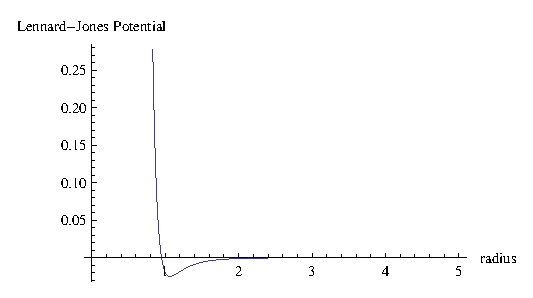
\includegraphics[width=3.45in]{lennardJonesPotential}
  \end{center}

  %\caption{\small Figure caption. To get a figure to span two columns, use the environment figure* rather than figure.}
  \caption{\small Lennard-Jones Potential}
  \label{fig:lennardJonesPotential}
\end{figure}

\section{System Model}
\label{sec:model}
For the system model, we are closely following the work of \cite{os2006}.
%
The system is composed of $N$ agents or nodes, each represented as a vertex in a set of vertices defined $V \subset \mathbb{N} = \{0 \ldots N \}$, of a graph $G := (V, \varepsilon)$, where the edges are defined as $\varepsilon \subseteq \{(i,j) : i,j \in V, j \neq i\}$.
%
The state-space representation of node $i \in V$ is $\dot{q}_i = p_i$, $\dot{p}_i = u_i$, where $q_i, p_i, u_i \in \mathbb{R}^m$, and $q_i$ represents position, $p_i$ represents velocity, and $u_i$ represents acceleration, or proportionally, force.
%
We denote the matrix of positions of all $N$ agents as $q \in \mathbb{R}^{m \times N}$, velocities as $p \in \mathbb{R}^{m \times N}$, and controls as $u \in \mathbb{R}^{m \times N}$.

The notion of nearby as flockmates being within some communications radius of one another gives rise to a definition of the \textit{communications neighbors} of agent $i$ as $N_c(i, q) := \{ j \in V : \norm{q_j - q_i} < r_{comm}\}$.
%
Each agent computes its own set of communications neighbors.
%
Similarly, the definition of a flock as agents being equidistantly spaced gives rise to the definition of a flock as an \textit{$\alpha$-lattice} as the solutions of the set of constraints $\norm{q_j - q_i} = r_{lattice}, \forall j \in N_c(i, q)$.
%
Alternatively, we could define the set of \textit{$\alpha$-lattice neighbors} as $N_l(i, q) := \{ j \in N_c(i, q) :  \norm{q_j - q_i} = r_{lattice}\}$.
%
This $\alpha$-lattice definition of flocking is overly restrictive though and disallows any small perturbations in the system, so we consider a quasi $\alpha$-lattice as $-\delta \leq \norm{q_j - q_i} - r_{lattice} \leq \delta, \forall j \in N_c(i, q)$.

We do not need to consider any deviation from a perfect $\alpha$-lattice in terms of some deviation energy, as this is required for stability proofs only, and is not used in the computation of an agent's control.
%
Similarly, for real-world implementations in software we would not have such rigorously defined functions as in \cite{os2006}, so we will depart to some extent from the work of Olfati-Saber at this point.
%
For analysis purposes and a proof of convergence to a flock, they carefully construct a continuous control.
%
For simulations we can define the $\sigma$-norm ($\mathbb{R}^m \rightarrow \mathbb{R}_{\geq 0}$) simply as the Euclidean norm ($2$-norm), $\norm{z}_{\sigma} := \sqrt{z_1^2 + \ldots + z_m^2}$, instead of $\norm{z}_{\sigma} = \frac{1}{\epsilon}\left[\sqrt{1 + \epsilon\norm{z}^2} - 1\right]$, for $\epsilon > 0$.  The difference is highlighted in Figure~\ref{fig:oldSigmaNorm} and Figure~\ref{fig:newSigmaNorm}.
%
Note however that we do take the same values of $r_{\alpha}$ (here $r_{comm}^{\alpha}$) and $d_{\alpha}$ (here $r_{lattice}^{\alpha}$) as though they were computed using their $\sigma$-norm, as otherwise it would be hard to compare results; these specific values are given in Section~\ref{sec:simulations}.

\begin{figure}[!htb]
  \begin{center}
    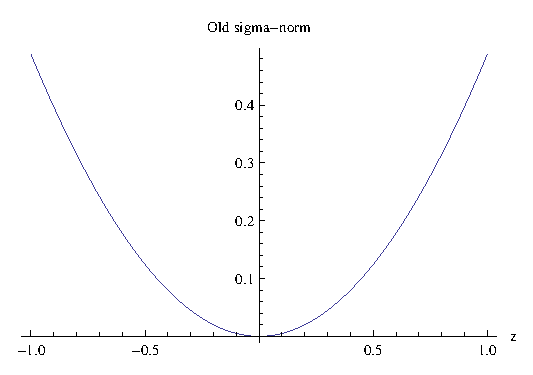
\includegraphics[width=3.45in]{sigmaNormOld}
  \end{center}

  %\caption{\small Figure caption. To get a figure to span two columns, use the environment figure* rather than figure.}
  \caption{\small Old $\sigma$-Norm}
  \label{fig:oldSigmaNorm}
\end{figure}

\begin{figure}[!b]
  \begin{center}
    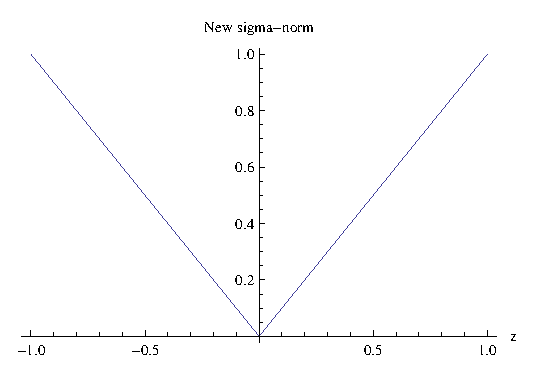
\includegraphics[width=3.45in]{sigmaNormNew}
  \end{center}

  \caption{\small New $\sigma$-Norm}
  \label{fig:newSigmaNorm}
\end{figure}

%
The gradient of the $\sigma$-norm, $\sigma_{\epsilon}(z) := \nabla \norm{z}_{\sigma}$, is needed, and becomes $\sigma_{\epsilon}(z) := \frac{z}{\norm{z}}$ instead of $\sigma_{\epsilon}(z) = \frac{z}{\sqrt{1 + \epsilon||z||^2}} = \frac{z}{1 + \epsilon||z||_{\sigma}}$.
%
This is no longer differentiable at $0$, but for simulations, this does not matter.

Similarly, the $C^1$-smooth bump function $\rho_{h}$ can be redefined as 

$\rho_{h}\left(z\right) = \left\{ \begin{array}{ll} 
1 & \textrm{if } z \in \left[0, h\right) \\
1 - z & \textrm{if } z \in \left[h, 1\right] \\
0 & \textrm{else} \end{array} \right. $\\
instead of as 

$\rho_{h}\left(z\right) = \left\{ \begin{array}{ll} 
1 & \textrm{if } z \in \left[0, h\right) \\
\frac{1}{2}\left[1 + cos\left(\pi\frac{\left(z - h\right)}{\left(1 - h\right)}\right)\right] & \textrm{if } z \in \left[h, 1\right] \\
0 & \textrm{else} \end{array} \right. $.\\
These differences are seen in Figure~\ref{fig:rhoHOld} and Figure~\ref{fig:rhoHNew}.

\begin{figure}[!b]
  \begin{center}
    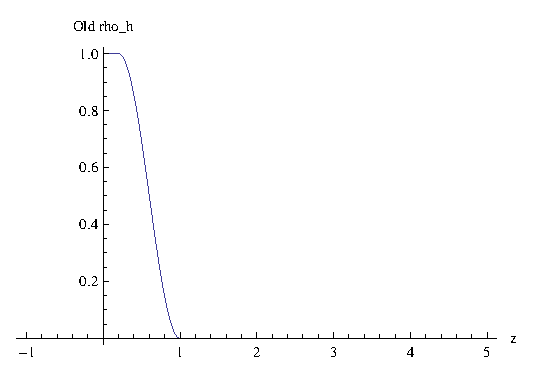
\includegraphics[width=3.45in]{rhoHOld}
  \end{center}

  \caption{\small Old $\rho_h$}
  \label{fig:rhoHOld}
\end{figure}

\begin{figure}[!b]
  \begin{center}
    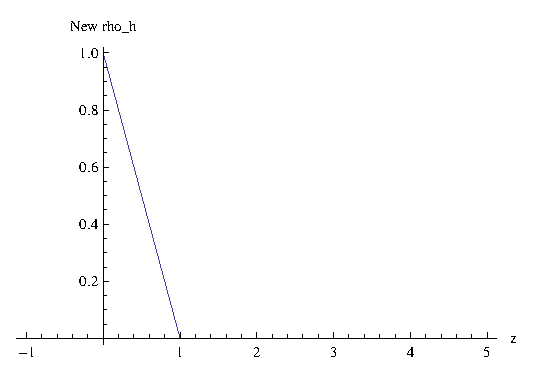
\includegraphics[width=3.45in]{rhoHNew}
  \end{center}

  \caption{\small New $\rho_h$}
  \label{fig:rhoHNew}
\end{figure}

Using these new functions, we work with the same element-wise definition of the \textit{spatial adjacency matrix}, $A := [a_{ij}]$, as Olfati-Saber, $a_{ij}\left(q\right) = \rho_{h}\left(\frac{\norm{q_j - q_i}_{\sigma}}{r_{lattice}^{\alpha}}\right) \in \left[0, 1\right], j \neq i$.
%
We also use the same $\phi$ and $\phi_{\alpha}$ functions, defined as $\phi(z) := \frac{1}{2}\left[(a+b)\sigma_1(z+c)+(a-b)\right]$ and $\phi_{\alpha}(z) := \rho_h(\frac{z}{r_{lattice}^{\alpha}})\phi(z - r_{comm}^{\alpha})$, where $\sigma_1(z) = \frac{z}{\sqrt{1 + z^2}}$, $0 < a \leq b$, and $c := \frac{\abs{a - b}}{\sqrt{4ab}}$.
%
Note that while these are defined the same, both have changed due to them being composed of other functions that have changed.
%
The change to $\phi$ is seen in Figure~\ref{fig:oldPhi} and Figure~\ref{fig:newPhi} and to $\phi_{\alpha}$ in Figure~\ref{fig:oldPhiAlpha} and Figure~\ref{fig:newPhiAlpha}.

\begin{figure}[!b]
  \begin{center}
    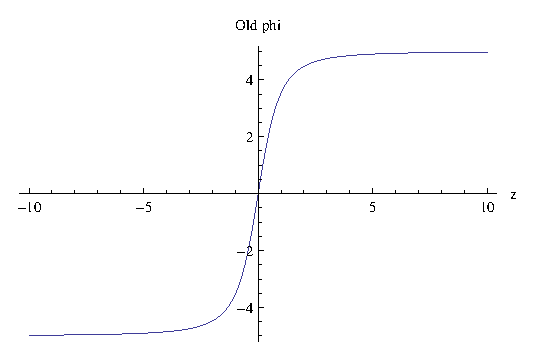
\includegraphics[width=3.45in]{phiOld}
  \end{center}

  \caption{\small Old $\phi$}
  \label{fig:oldPhi}
\end{figure}

\begin{figure}[!b]
  \begin{center}
    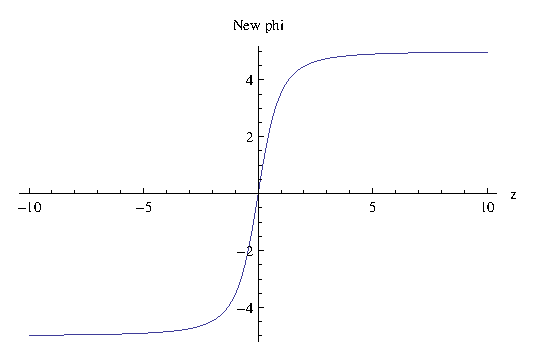
\includegraphics[width=3.45in]{phiNew}
  \end{center}

  \caption{\small New $\phi$}
  \label{fig:newPhi}
\end{figure}

\begin{figure}[!b]
  \begin{center}
    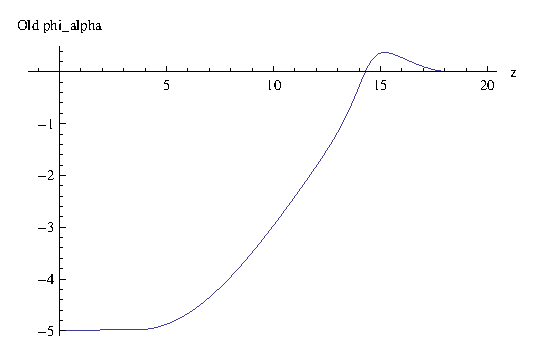
\includegraphics[width=3.45in]{phiAlphaOld}
  \end{center}

  \caption{\small Old $\phi_{\alpha}$}
  \label{fig:oldPhiAlpha}
\end{figure}

\begin{figure}[!b]
  \begin{center}
    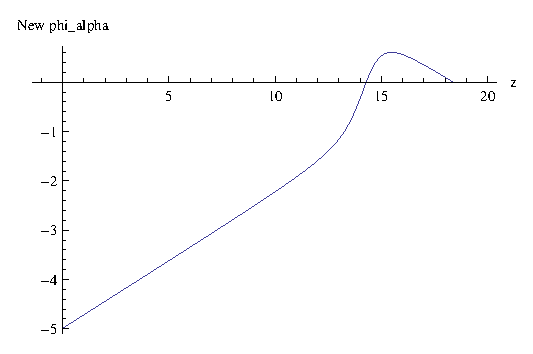
\includegraphics[width=3.45in]{phiAlphaNew}
  \end{center}

  \caption{\small New $\phi_{\alpha}$}
  \label{fig:newPhiAlpha}
\end{figure}

We focus only on the control in the form of \textit{Algorithm 2} presented in \cite{os2006}, which is defined as $u_i := u_i^\alpha + u_i^\gamma$, where\\
$u_i^\alpha = \displaystyle\sum_{j \in N_c(i,q)}\phi_{\alpha}\left(\norm{q_j - q_i}_{\sigma}\right)n_{ij} + \displaystyle\sum_{j \in N_c(i,q)}a_{ij}(q)(p_j - p_i)$\\
and
%
$u_i^\gamma = f_i^{\gamma}(q_i, p_i, q_r, p_r)=-c_1(q_i - q_r) - c_2(p_i - p_r)$ with $q_r$ and $p_r$ representing the state of the goal, which may be changing, and where $n_{ij} := \frac{\left(q_j - q_i\right)}{\sqrt{1 + \epsilon \norm{q_j - q_i}^2}}$, $c_1 > 0$, and $c_2 > 0$.
%
The goal's dynamic state is modeled as a double integrator also, with state-space representation $\dot{q}_r = p_r$ and $\dot{p}_r = f_r(q_r, p_r)$.
%
Note that we have taken $f_r(q_r, p_r) \equiv 0$, although it could be any function, such as one that sets different objectives at discrete points in time.

\subsection{System Constraints}
\label{sec:constraints}

\subsubsection{State and Actuator Saturation}

There exists $v_{max}$ and $a_{max}$, a maximum velocity and acceleration, respectively, such that, $\norm{\dot{q}_{i}} \leq v_{max}$ and $\norm{\dot{p}_{i}} \leq a_{max}$.
%
The existence of a maximum acceleration is reasonable given that it would be produced by some actuator with limited operating range and power source.
%
Note that of course the existence of a maximum acceleration does not imply the existence of a maximum velocity.
%
However, the existence of a maximum force that can be applied as a control, which is proportional to the maximum acceleration, and in the presence of opposing forces proportional to the velocity such that $\sum{F}=0$ where $F \in \mathbb{R}^m$, does imply the existence of a maximum velocity, so this is a reasonable assumption.
%
On Earth the balancing forces could be aerodynamic resistance, whereas in space, relativistic limits could be imposed.

For the simulations in Section~\ref{sec:simulations}, we separately present results with state and actuator saturation.
%
In general, actuator saturation is quite interesting, as it reduces any globally asymptotically stable system to (at best) a locally asymptotically stable system.
%
Coupled with state constraints though, the problem is even more interesting, as not all of $\mathbb{R}^m$ is accessible by the states anyway, so all \textit{reachable states} may be asymptotically stable nonetheless.
%
These constraints were primarily motivated by previous work of ours on finding stabilizable regions by solving LMIs for an inverted pendulum system with limited actuator range, and with a limited set of safe states.

\subsubsection{Delayed State Feedback}

No communications in the real world can occur instantaneously, so we consider delayed feedback of state information, such as that which would be experienced by nodes transmitting their positions over a wireless network, or, of the delay necessary for local sensory information to become available.
%
As each node computes its own control based on the positions and velocities of nodes around it at an instant of time, the control update must utilize old state information of the agents within the communications radius.
%
There are many results in this area, but we are most familiar with the theoretical foundation in \cite{LiberzonQuantDelay2006}, where a small-gain criteria is established to prove asymptotic stability for sufficiently small delays and quantization errors.

\section{Simulations}
\label{sec:simulations}

We created a simulation framework based around the \textit{Algorithm 2} of Olfati-Saber, with the control and simulation environment designed for $m$-dimensional systems.
%
We present a few samples of $1$-dimensional and $3$-dimensional simulations in Figures~\ref{fig:simOneDt00} to \ref{fig:simOneDt32} and Figures~\ref{fig:simThreeDt00} to \ref{fig:simThreeDt36}, respectively.
%
For all other simulations, we work in $2$ dimensions ($m=2$) with $N=50$ agents.
%
For all simulations except where otherwise noted, the sampling period (the time between control updates for a node) is $T_c = 0.01$ seconds.
%
Other constants used in the above definition of the controls are $a=5$, $b=5$, $c=0$, $\epsilon=0.1$, $h=h_a = 0.2$, and $h_b = 0.9$.
%
The communications radius is set at $r_{comm}=8.4m$ and the lattice distance is set at $r_{lattice}=7m$ with the quasi-$\alpha$ lattice constant set at $\delta=1.4m$.
%
The constants used to weight the importance of the goal position and velocity in the $u_i^{\gamma}$ term are $c_1=c_2=0.1$; these are not listed in the \cite{os2006} paper, but have a drastic impact on the results of simulation.
%
All nodes start from random initial positions, $q_0$, located in the box $[0m, 100m]$ for each dimension, and each is represented as a \textit{green} circle from a scatter plot with a \textit{green} arrow representing the velocity vector from a quiver plot.
%
If nodes are in a quasi-$\alpha$ lattice, the lattice will be drawn in \textit{blue}.
%
The objective is $q_r=[100m, 100m]$, $p_r=[\frac{v_{max}m/s}{5} \frac{v_{max}}{5}m/s]$, so it is moving over time; it is represented in \textit{red} in the plots.
%
There is a small errata note here: we recently found a bug in the way maximum acceleration and velocity were limited--rather than the norm being limited, each dimension is limited to the maximum value, so all the results hold, just by an increase of a norm of the $v_{max}$ and $a_{max}$ from the values given; this also explains why the red objective arrow is often differently sized than the individual nodes.

\subsection{Without Constraints}

Before presenting results with constraints, we must first look at simulations without constraints for comparison.  Figures~\ref{fig:n50m2t00} to \ref{fig:n50m2t32} are a representative example, showing the system with $50$ agents starting from random initial positions as described above, and with velocities in the range $-100m/s$ to $100m/s$.
%
The control value, separated into components, of one node over time can be seen in Figure~\ref{fig:n50m2control}.
%
The norm of the position value of all nodes as a function of time can be seen in Figure~\ref{fig:n50m2position}; this plot can be particularly useful if one wants to verify more stringent properties, such as two agents never coming closer than some small amount within one another (of course this occurs with this control, but with a different setup, it may not).
%
It is also useful to look at this plot for simple convergence of nodes to the moving goal, as they form a regular spacing if they are properly in a flock.

\begin{figure}[!h]
  \begin{center}
    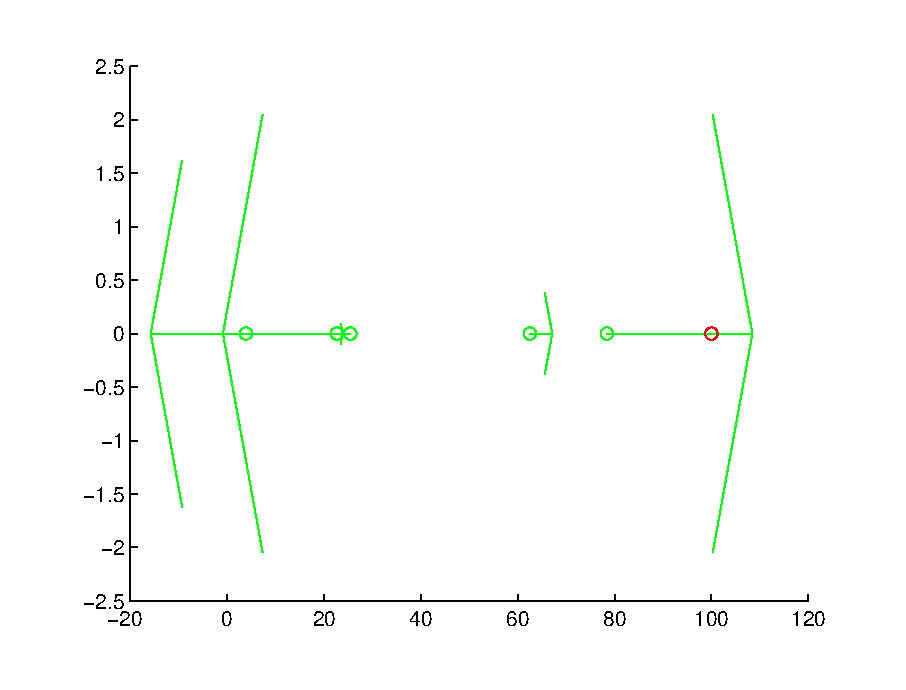
\includegraphics[width=3.45in]{simOneDt00}
  \end{center}

  \caption{\small N=10, m=1, Time=0s}
  \label{fig:simOneDt00}
\end{figure}

\begin{figure}[!p]
  \begin{center}
    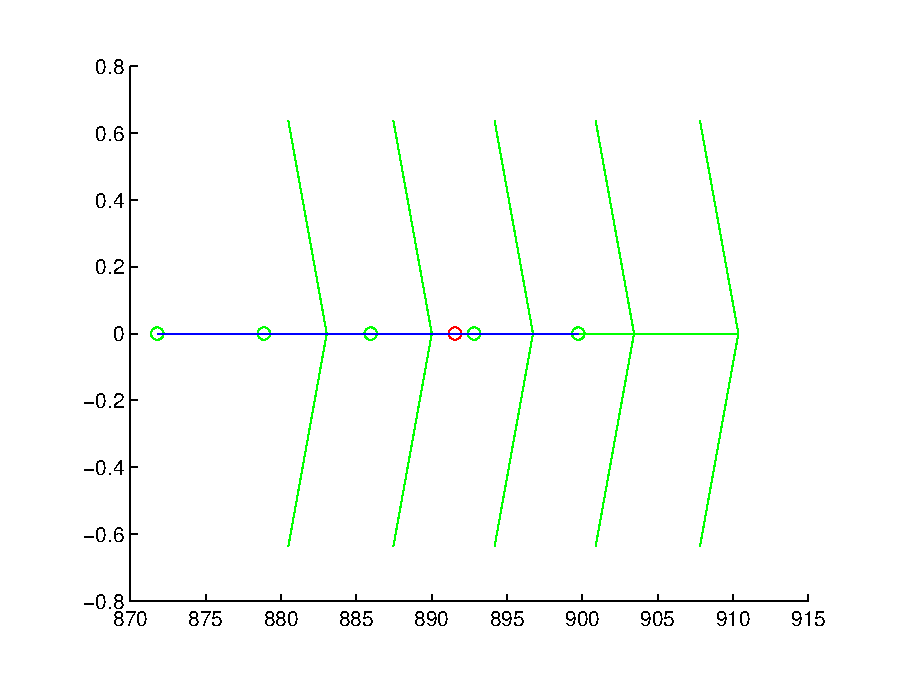
\includegraphics[width=3.45in]{simOneDt32}
  \end{center}

  \caption{\small N=10, m=1, Time=32s}
  \label{fig:simOneDt32}
\end{figure}

\begin{figure}[!p]
  \begin{center}
    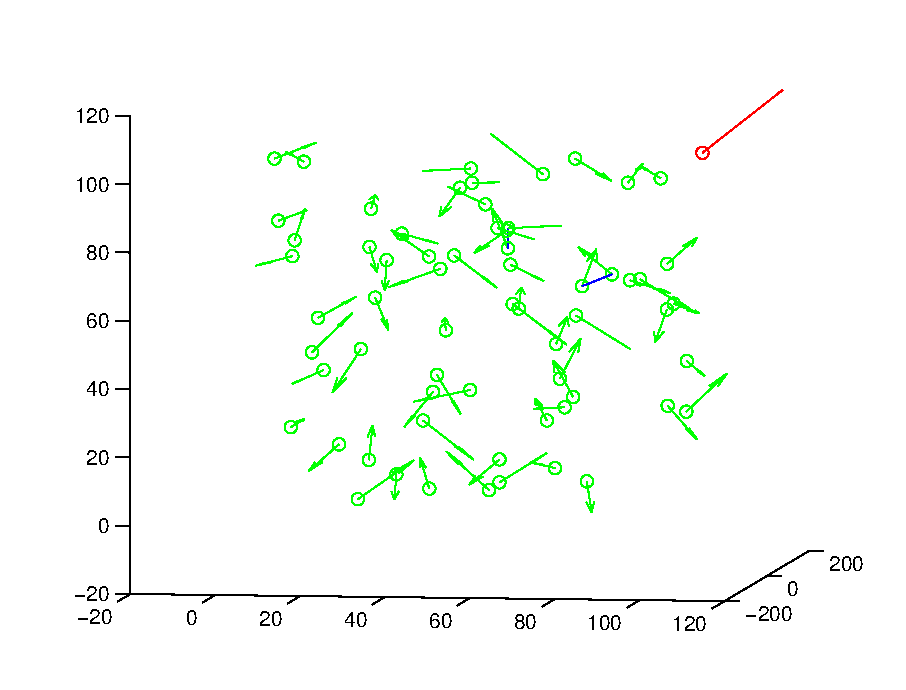
\includegraphics[width=3.45in]{simThreeDt00}
  \end{center}

  \caption{\small N=64, m=3, Time=0s}
  \label{fig:simThreeDt00}
\end{figure}

\begin{figure}[!p]
  \begin{center}
    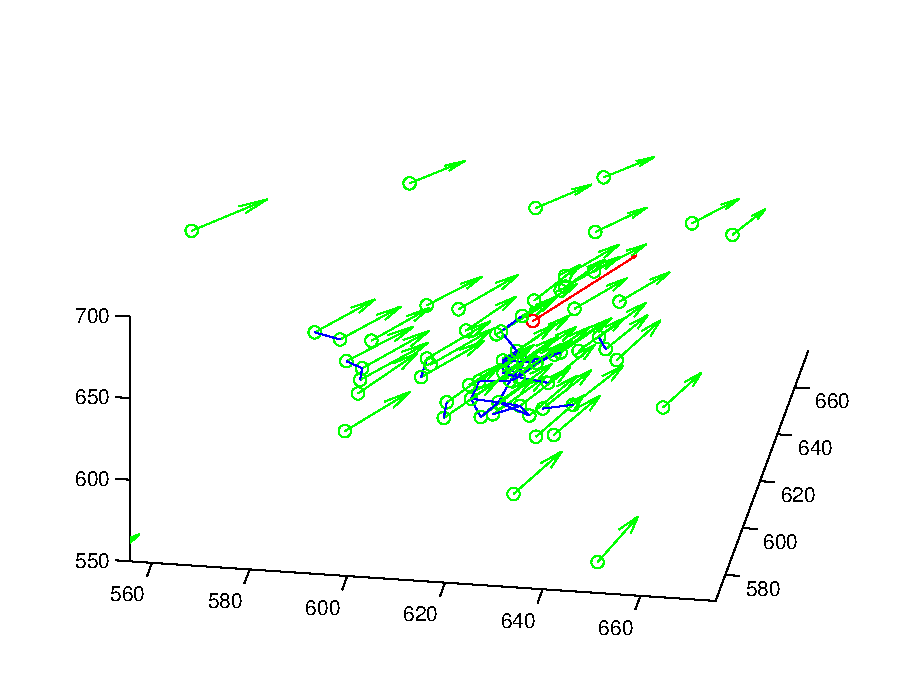
\includegraphics[width=3.45in]{simThreeDt24}
  \end{center}

  \caption{\small N=64, m=3, Time=24s}
  \label{fig:simThreeDt24}
\end{figure}

\begin{figure}[!p]
  \begin{center}
    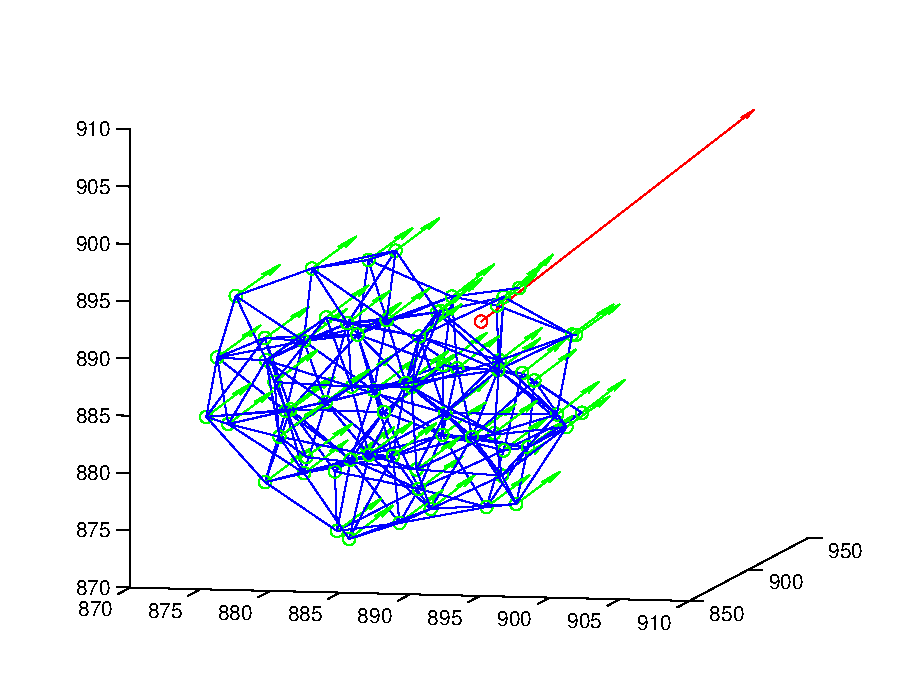
\includegraphics[width=3.45in]{simThreeDt36}
  \end{center}

  \caption{\small N=64, m=3, Time=36s}
  \label{fig:simThreeDt36}
\end{figure}

\clearpage

\begin{figure}[!p]
  \begin{center}
    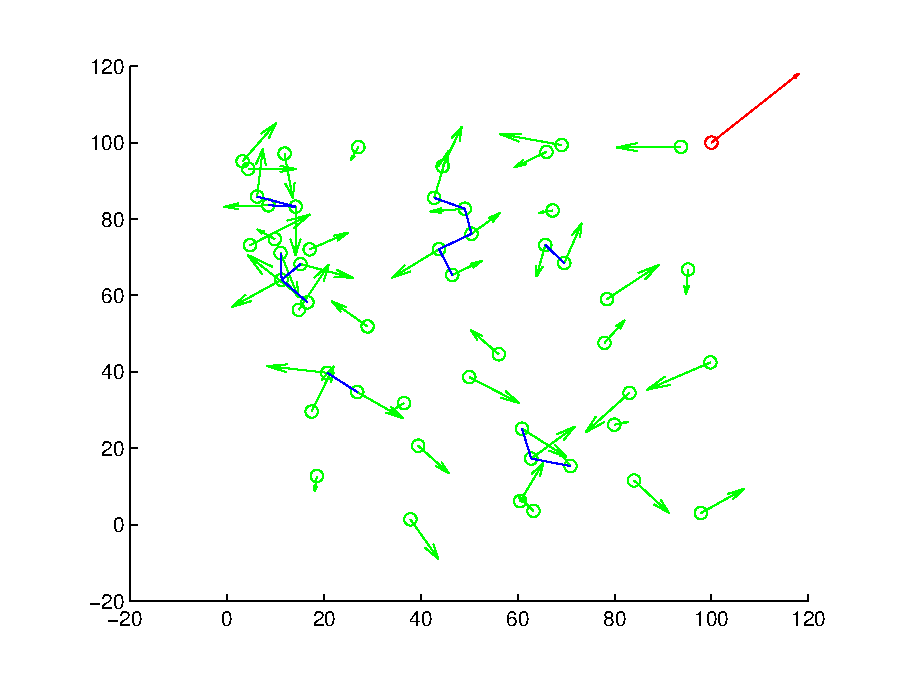
\includegraphics[width=3.45in]{n50m2t00}
  \end{center}

  \caption{\small N=50, m=2, Time=0s}
  \label{fig:n50m2t00}
\end{figure}

\begin{figure}[!p]
  \begin{center}
    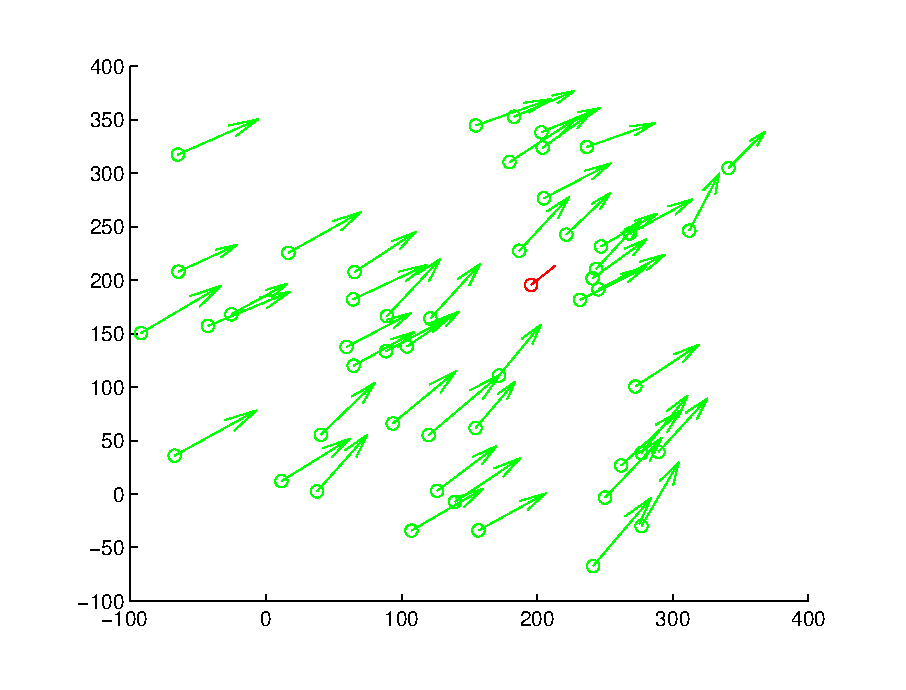
\includegraphics[width=3.45in]{n50m2t04}
  \end{center}

  \caption{\small N=50, m=2, Time=4s}
  \label{fig:n50m2t04}
\end{figure}

\begin{figure}[!p]
  \begin{center}
    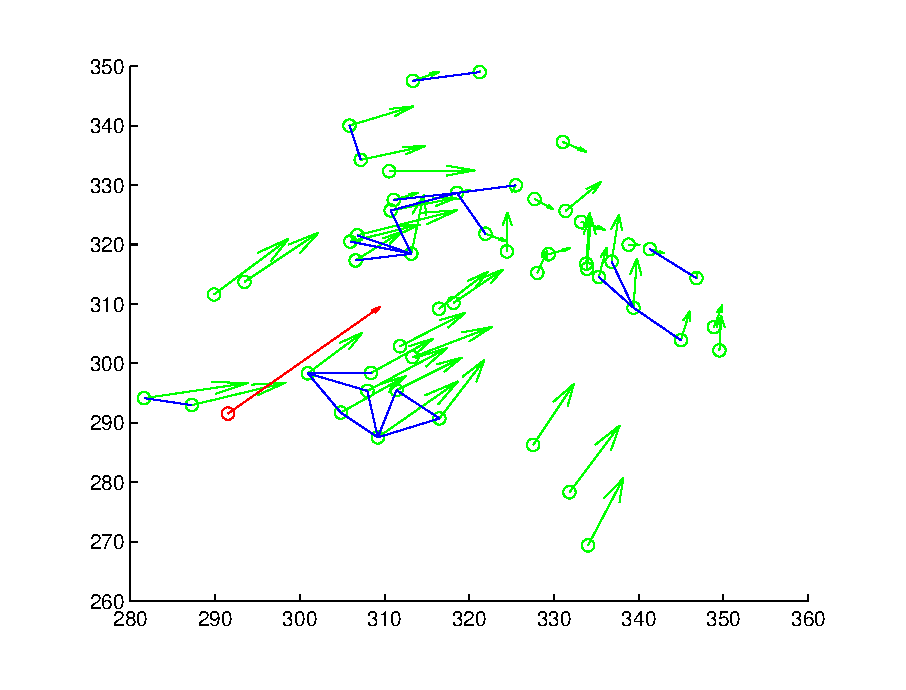
\includegraphics[width=3.45in]{n50m2t08}
  \end{center}

  \caption{\small N=50, m=2, Time=8s}
  \label{fig:n50m2t08}
\end{figure}

\begin{figure}[!p]
  \begin{center}
    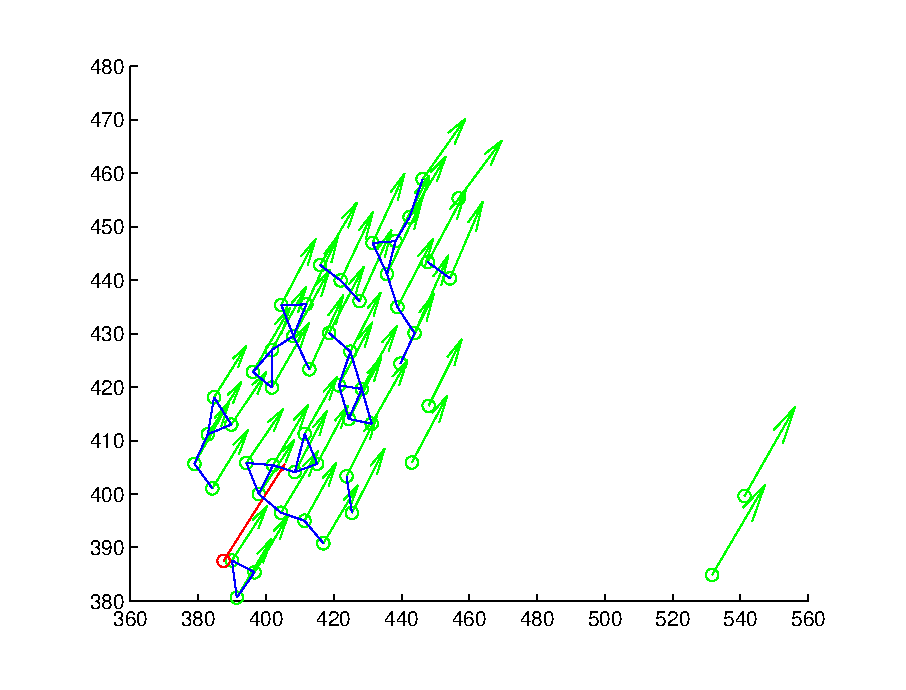
\includegraphics[width=3.45in]{n50m2t12}
  \end{center}

  \caption{\small N=50, m=2, Time=12s}
  \label{fig:n50m2t12}
\end{figure}

\begin{figure}[!p]
  \begin{center}
    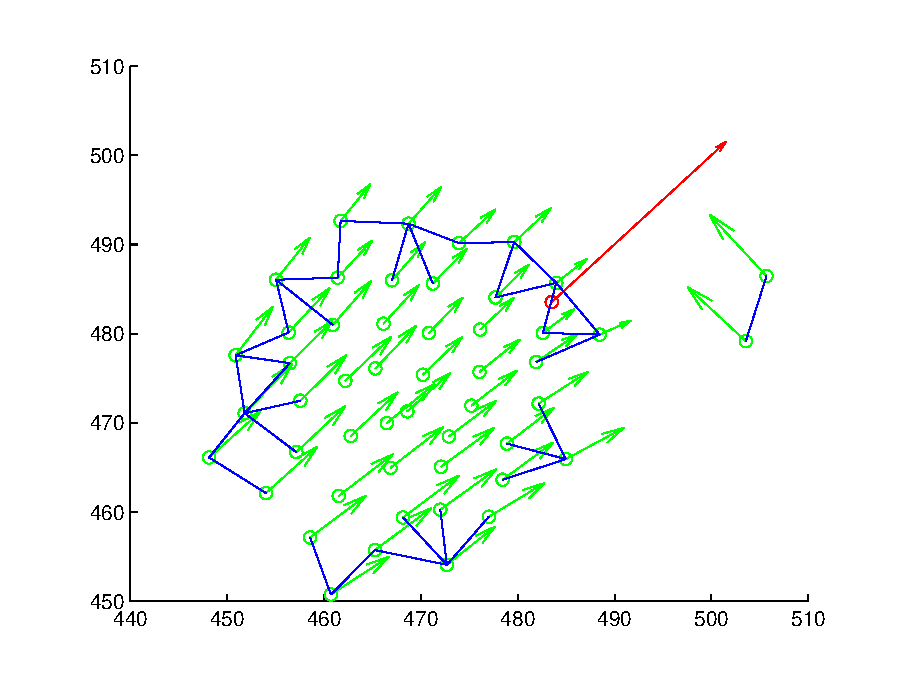
\includegraphics[width=3.45in]{n50m2t16}
  \end{center}

  \caption{\small N=50, m=2, Time=16s}
  \label{fig:n50m2t16}
\end{figure}

\begin{figure}[!p]
  \begin{center}
    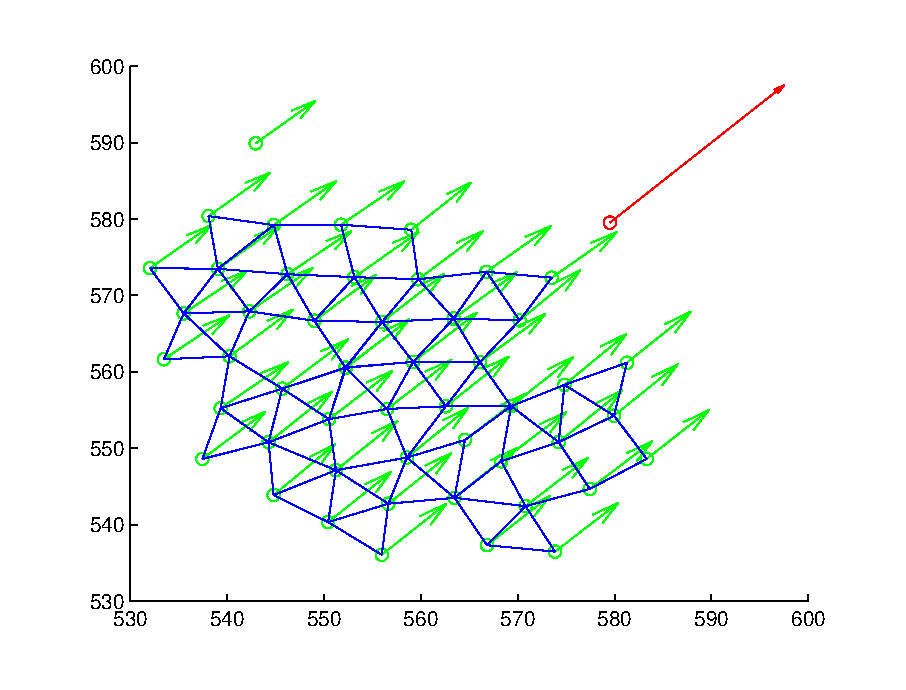
\includegraphics[width=3.45in]{n50m2t20}
  \end{center}

  \caption{\small N=50, m=2, Time=20s}
  \label{fig:n50m2t20}
\end{figure}

\begin{figure}[!p]
  \begin{center}
    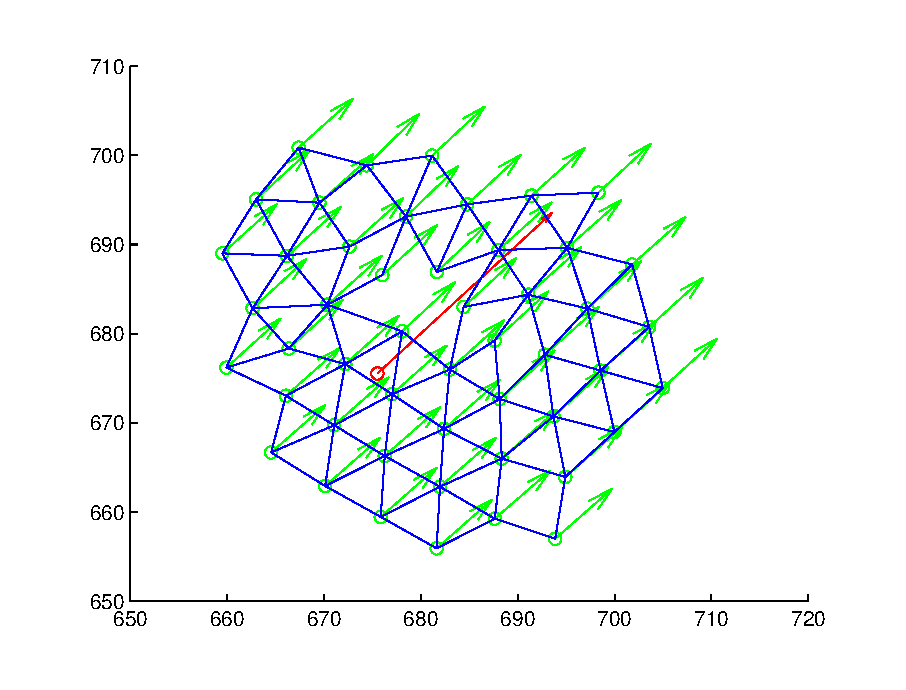
\includegraphics[width=3.45in]{n50m2t24}
  \end{center}

  \caption{\small N=50, m=2, Time=24s}
  \label{fig:n50m2t24}
\end{figure}

\begin{figure}[!p]
  \begin{center}
    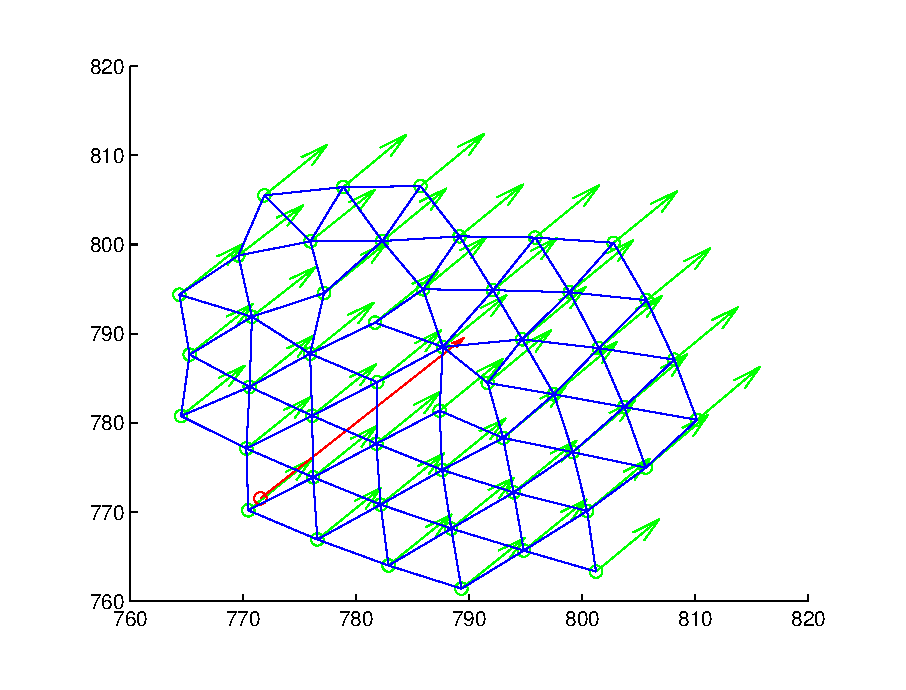
\includegraphics[width=3.45in]{n50m2t28}
  \end{center}

  \caption{\small N=50, m=2, Time=28s}
  \label{fig:n50m2t28}
\end{figure}

\begin{figure}[!p]
  \begin{center}
    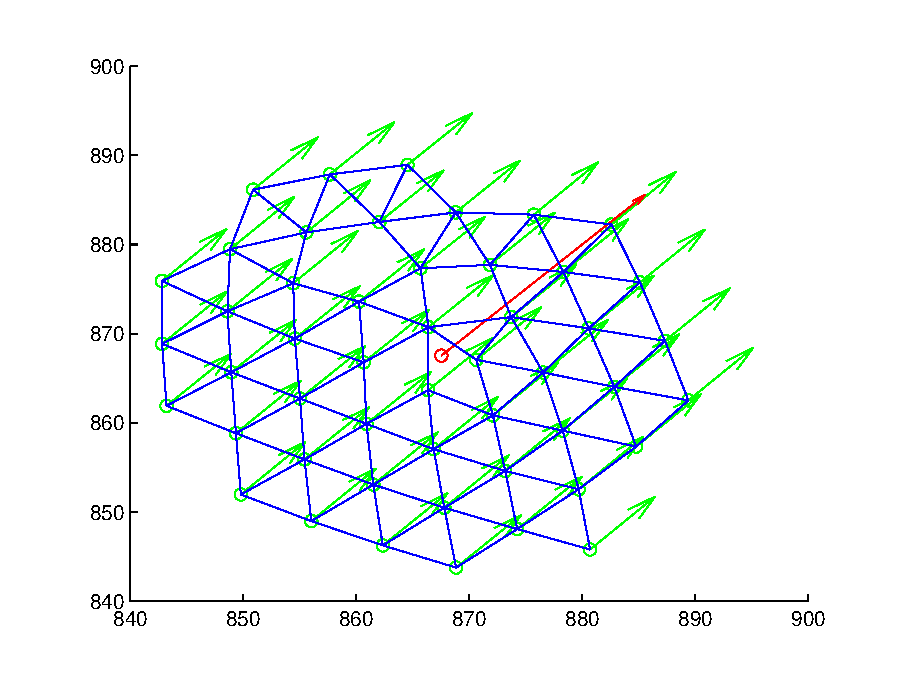
\includegraphics[width=3.45in]{n50m2t32}
  \end{center}

  \caption{\small N=50, m=2, Time=32s}
  \label{fig:n50m2t32}
\end{figure}

\begin{figure}[!p]
  \begin{center}
    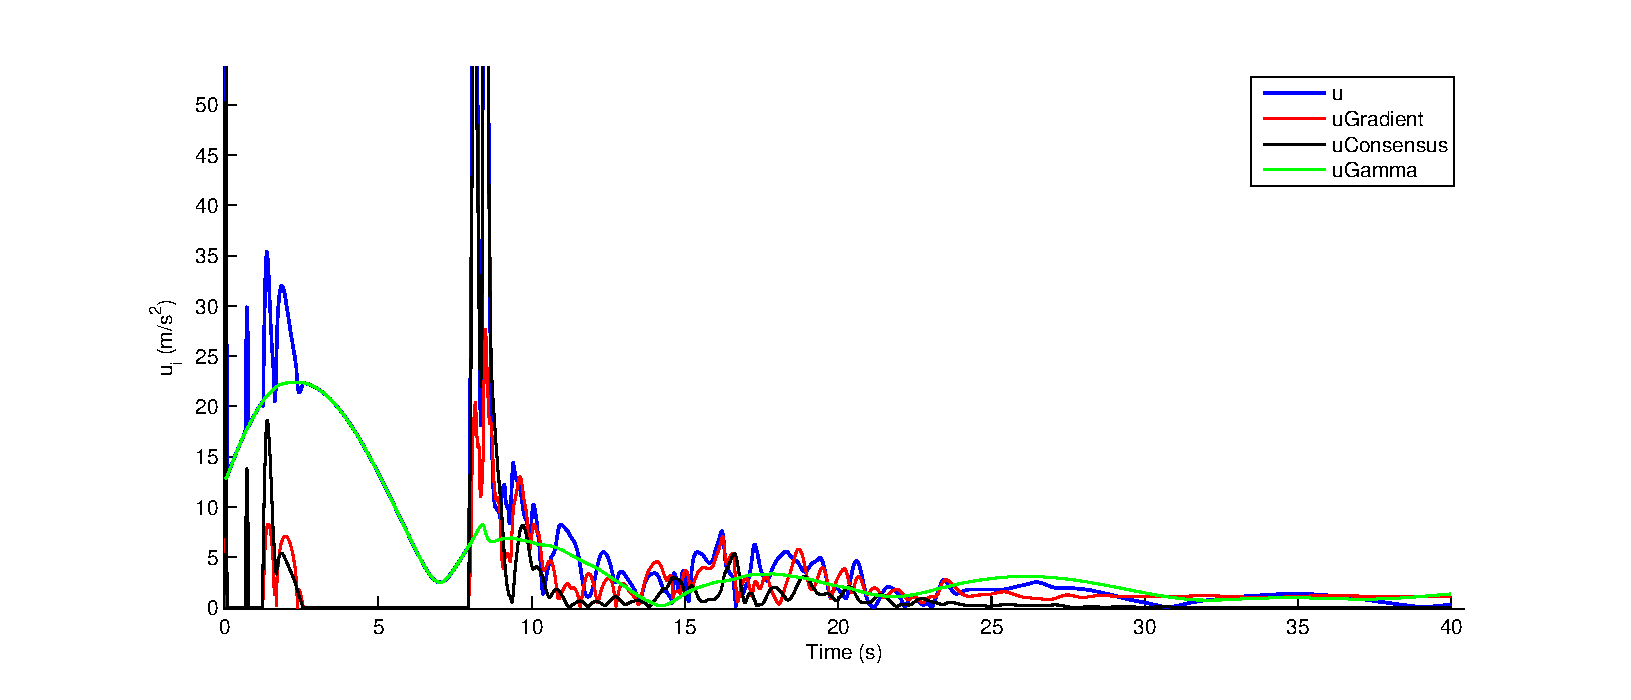
\includegraphics[width=3.45in]{n50m2control}
  \end{center}

  \caption{\small N=50, m=2, Control Value of One Node over Time}
  \label{fig:n50m2control}
\end{figure}

\begin{figure}[!p]
  \begin{center}
    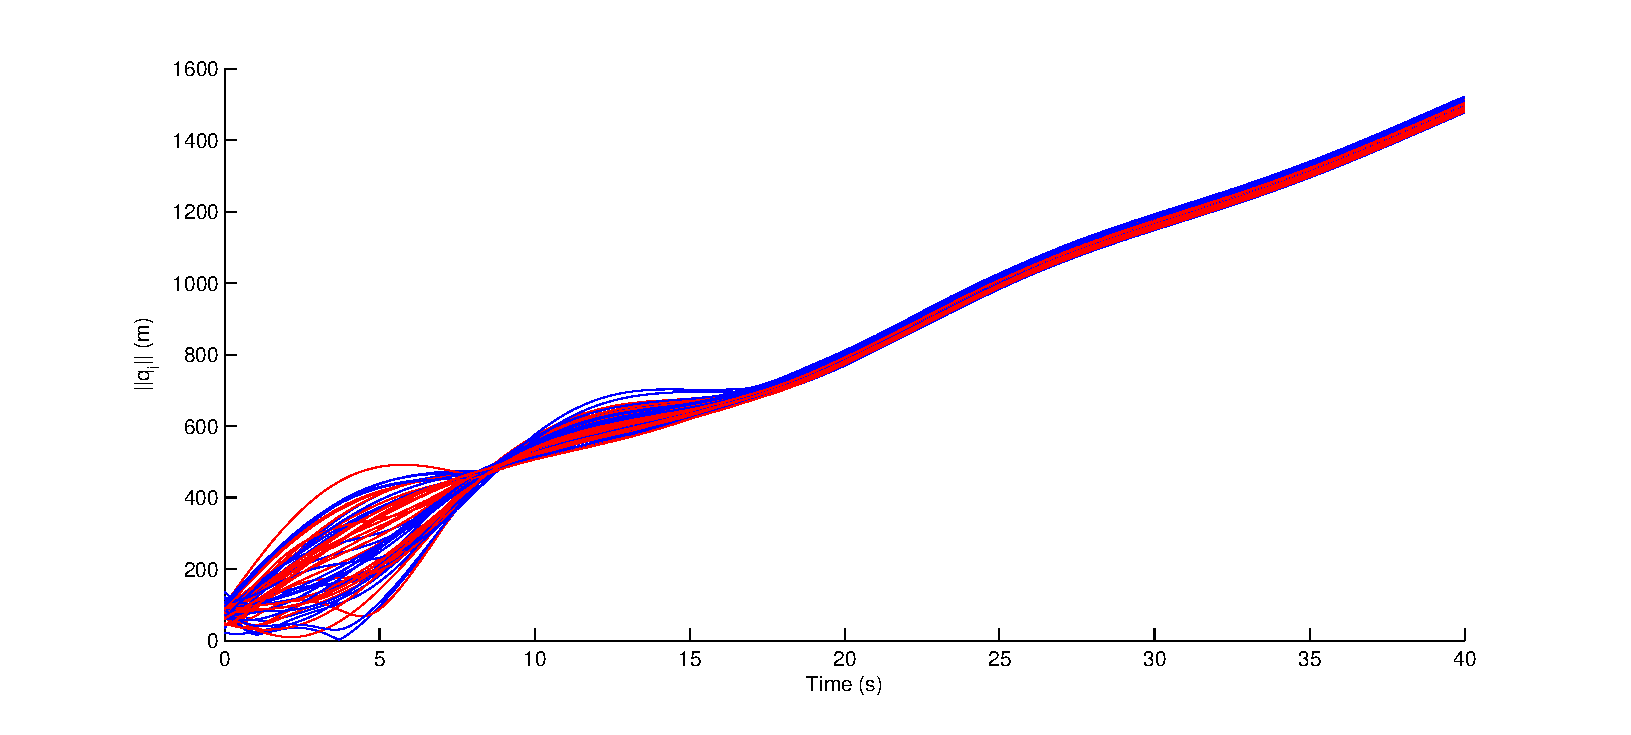
\includegraphics[width=3.45in]{n50m2position}
  \end{center}

  \caption{\small N=50, m=2, Position Values of All Nodes over Time}
  \label{fig:n50m2position}
\end{figure}

\clearpage

\subsection{State and Actuator Constraints}

Many simulations with constrained state were run, but for sake of presentation we show a comparison of a low maximum velocity ($v_{max} \equiv 1m/s$) in Figures~\ref{fig:n50m2vmax1t00} to \ref{fig:n50m2vmax1t32}, and the control can be seen in Figure~\ref{fig:n50m2vmax1control}.
%
Actuator constraint simulation with $a_{max} \equiv 1m/s^2$ can be seen in Figures~\ref{fig:n50m2vmax1000amax1t00} to \ref{fig:n50m2vmax1000amax1t32}.

\begin{figure}[!h]
  \begin{center}
    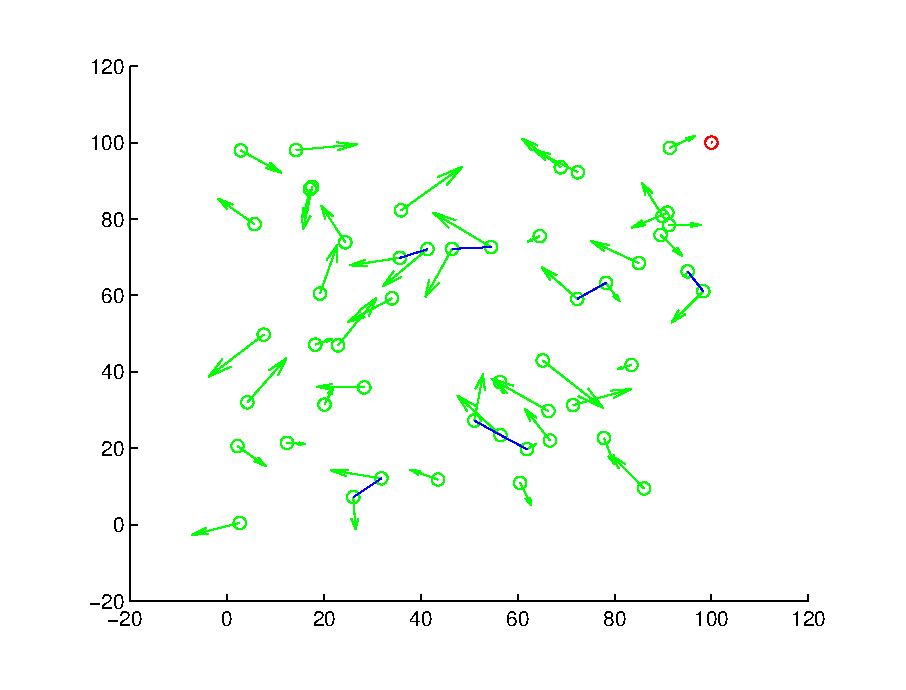
\includegraphics[width=3.45in]{n50m2vmax1t00}
  \end{center}

  \caption{\small N=50, m=2, Time=0s, $v_{max}=1m/s$}
  \label{fig:n50m2vmax1t00}
\end{figure}

\begin{figure}[!h]
  \begin{center}
    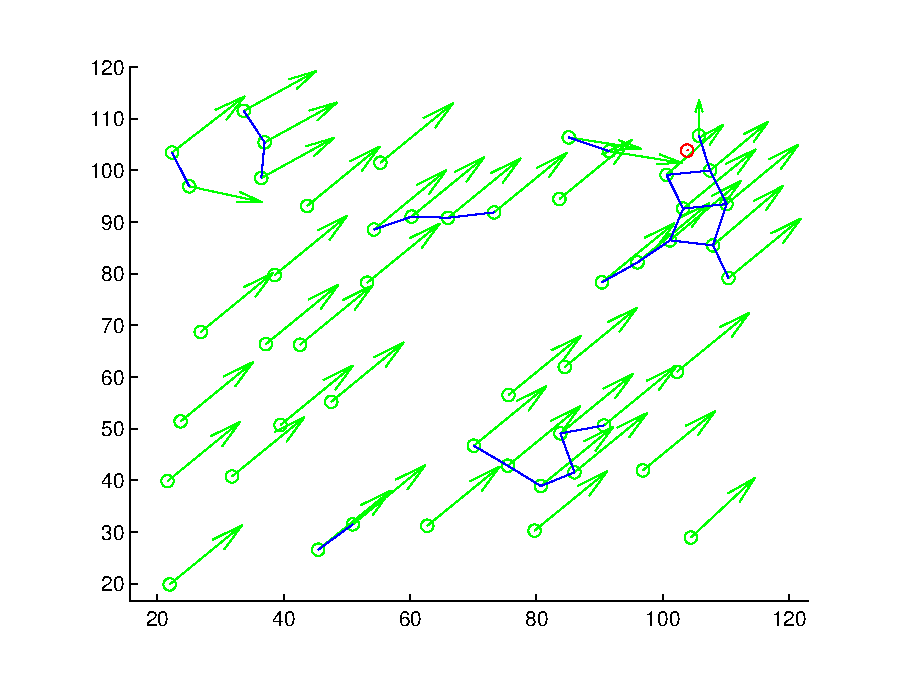
\includegraphics[width=3.45in]{n50m2vmax1t16}
  \end{center}

  \caption{\small N=50, m=2, Time=16s, $v_{max}=1m/s$}
  \label{fig:n50m2vmax1t16}
\end{figure}

\begin{figure}[!h]
  \begin{center}
    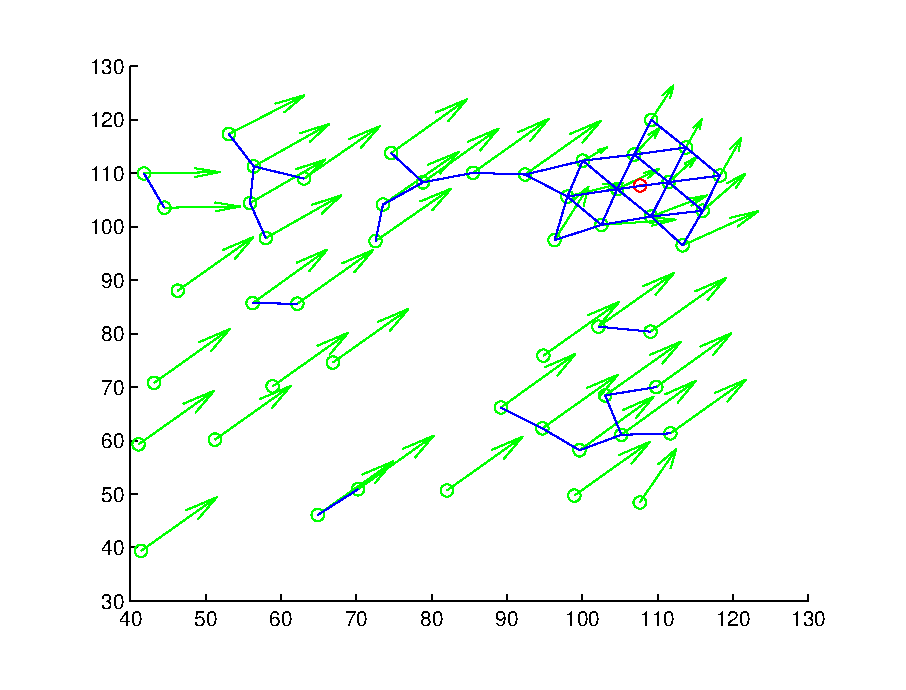
\includegraphics[width=3.45in]{n50m2vmax1t32}
  \end{center}

  \caption{\small N=50, m=2, Time=32s, $v_{max}=1m/s$}
  \label{fig:n50m2vmax1t32}
\end{figure}

\begin{figure}[!h]
  \begin{center}
    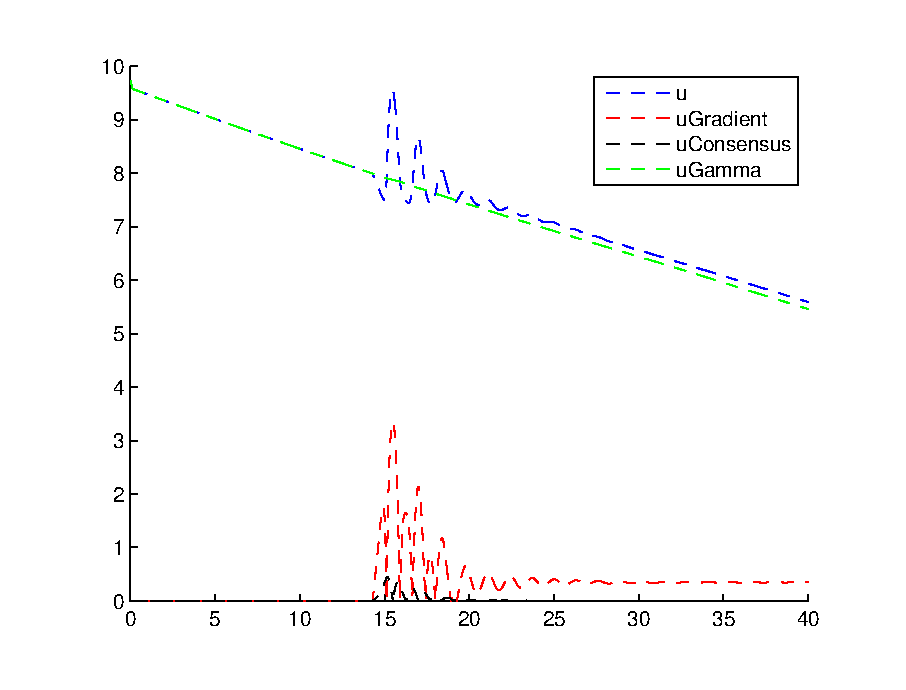
\includegraphics[width=3.45in]{n50m2vmax1control}
  \end{center}

  \caption{\small N=50, m=2, Control Value of One Node over Time, $v_{max}=1m/s$}
  \label{fig:n50m2vmax1control}
\end{figure}

%state and actuator

\clearpage

\begin{figure}[!h]
  \begin{center}
    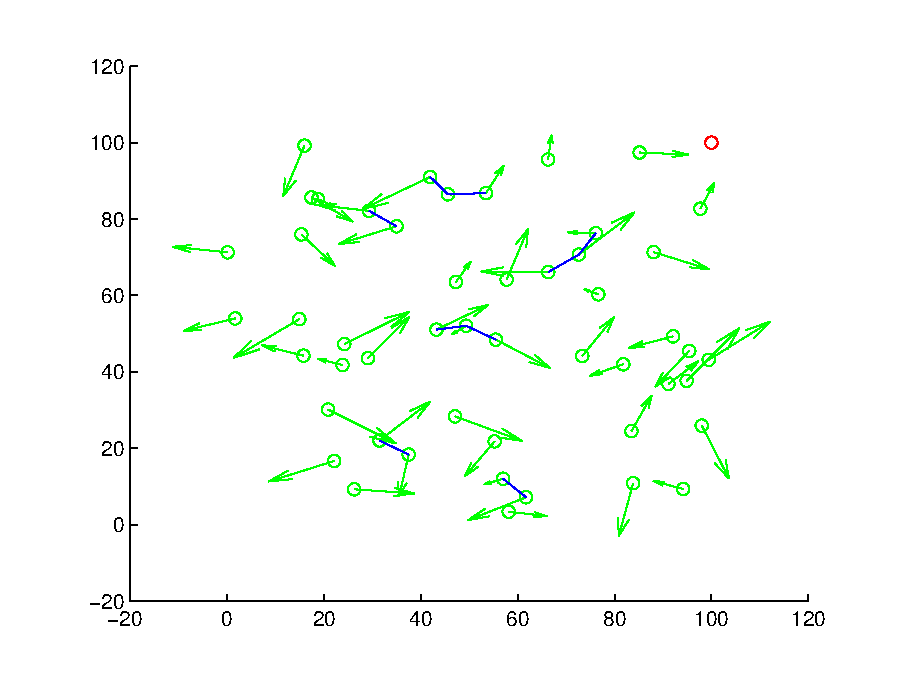
\includegraphics[width=3.45in]{n50m2vmax1000amax1t00}
  \end{center}

  \caption{\small N=50, m=2, Time=0s, $a_{max}=1m/s^2$}
  \label{fig:n50m2vmax1000amax1t00}
\end{figure}

\begin{figure}[!h]
  \begin{center}
    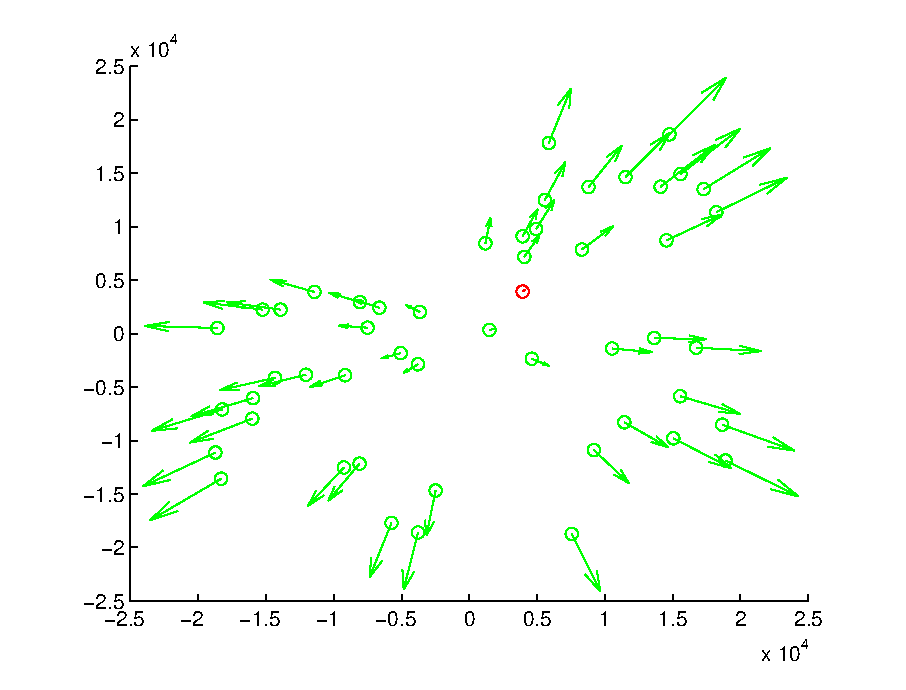
\includegraphics[width=3.45in]{n50m2vmax1000amax1t16}
  \end{center}

  \caption{\small N=50, m=2, Time=16s, $a_{max}=1m/s^2$}
  \label{fig:n50m2vmax1000amax1t16}
\end{figure}

\begin{figure}[!h]
  \begin{center}
    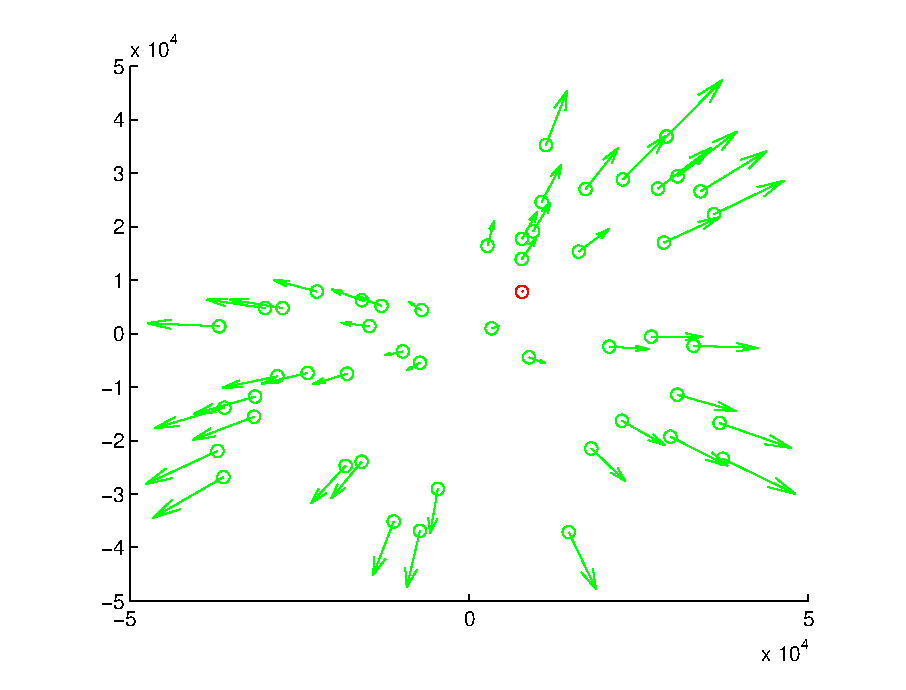
\includegraphics[width=3.45in]{n50m2vmax1000amax1t32}
  \end{center}

  \caption{\small N=50, m=2, Time=32s, $a_{max}=1m/s^2$}
  \label{fig:n50m2vmax1000amax1t32}
\end{figure}

\clearpage

\subsection{Delayed State Feedback}

Simulations with delayed state feedback, where nodes are using old state information of neighbors, is presented in Figures~\ref{fig:n50m2vmax100amax1000t00delay} to \ref{fig:n50m2vmax100amax1000t32delay}.
%
Actuator and velocity values were constrained, although to a very reasonable set, $v_{max}=100m/s$ and $a_{max}=1000m/s^2$, so that the actuator could quickly respond to any state changes.
%
The amount of delay experienced was always between one and two sampling periods ($T_c$ to $2T_c$, where $T_c = 0.1s$).

\begin{figure}[!h]
  \begin{center}
    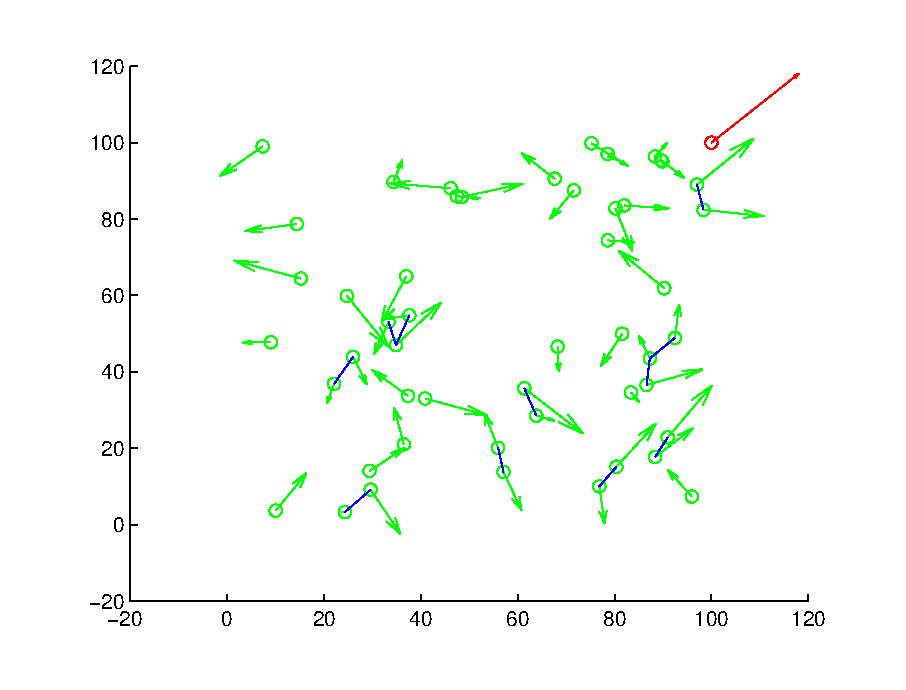
\includegraphics[width=3.45in]{n50m2vmax100amax1000t00delay}
  \end{center}

  \caption{\small N=50, m=2, Time=0s, Delayed}
  \label{fig:n50m2vmax100amax1000t00delay}
\end{figure}

\begin{figure}[!h]
  \begin{center}
    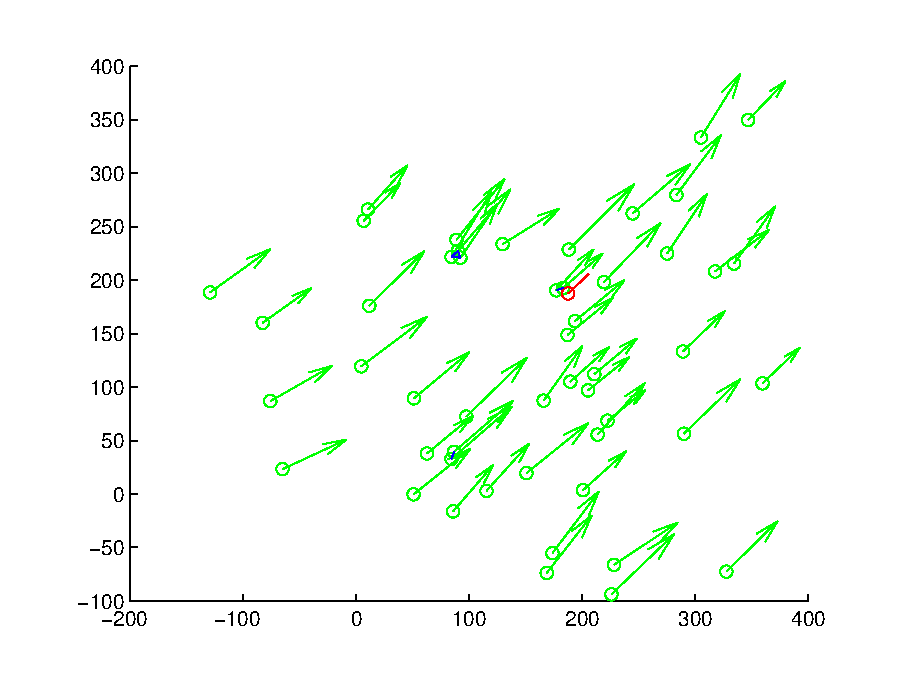
\includegraphics[width=3.45in]{n50m2vmax100amax1000t04delay}
  \end{center}

  \caption{\small N=50, m=2, Time=4s, Delayed}
  \label{fig:n50m2vmax100amax1000t04delay}
\end{figure}

\begin{figure}[!h]
  \begin{center}
    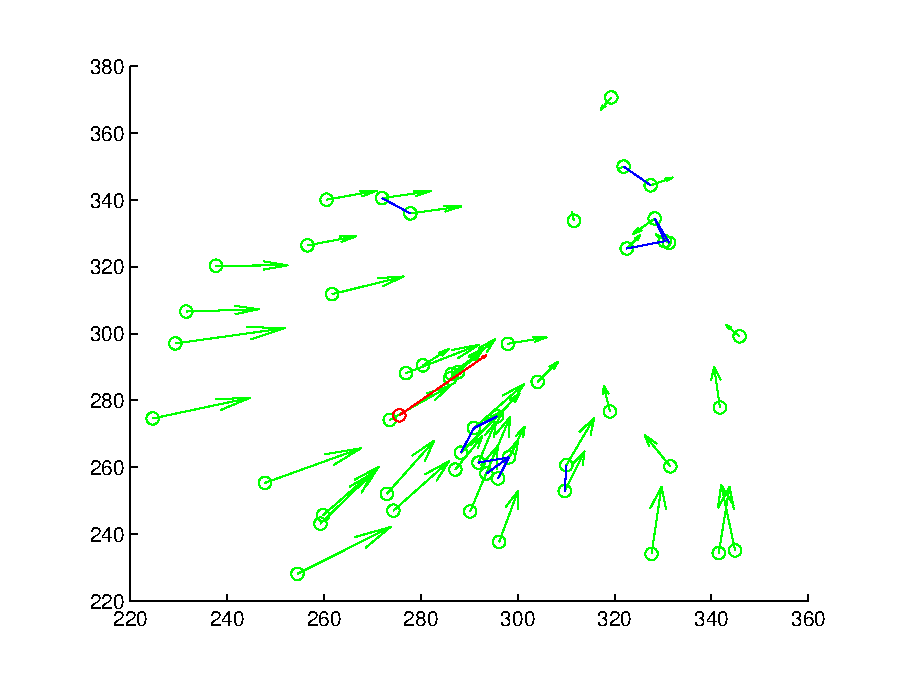
\includegraphics[width=3.45in]{n50m2vmax100amax1000t08delay}
  \end{center}

  \caption{\small N=50, m=2, Time=8s, Delayed}
  \label{fig:n50m2vmax100amax1000t08delay}
\end{figure}

\begin{figure}[!h]
  \begin{center}
    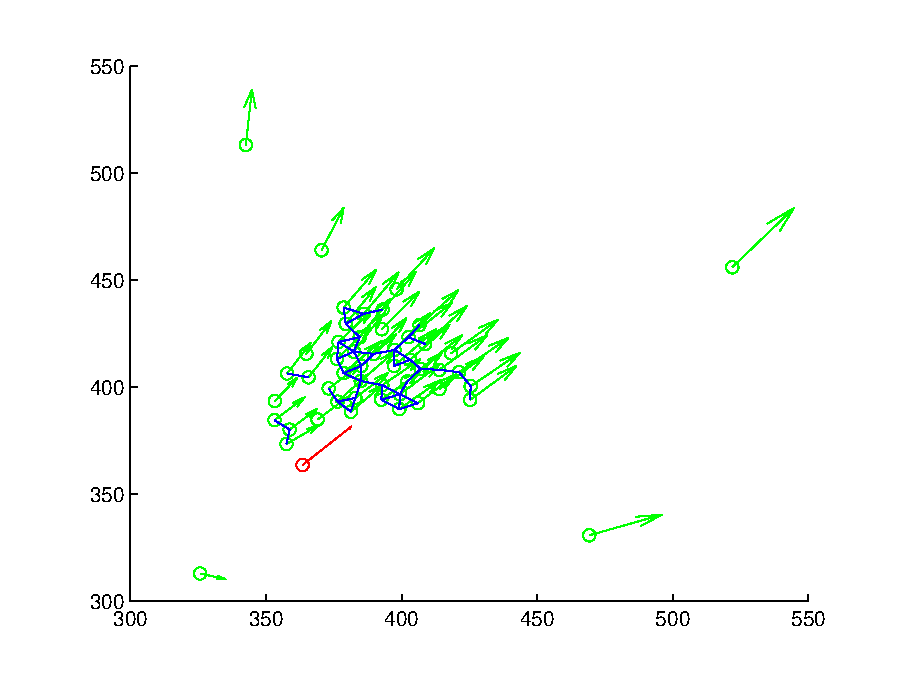
\includegraphics[width=3.45in]{n50m2vmax100amax1000t12delay}
  \end{center}

  \caption{\small N=50, m=2, Time=12s, Delayed}
  \label{fig:n50m2vmax100amax1000t12delay}
\end{figure}

\begin{figure}[!h]
  \begin{center}
    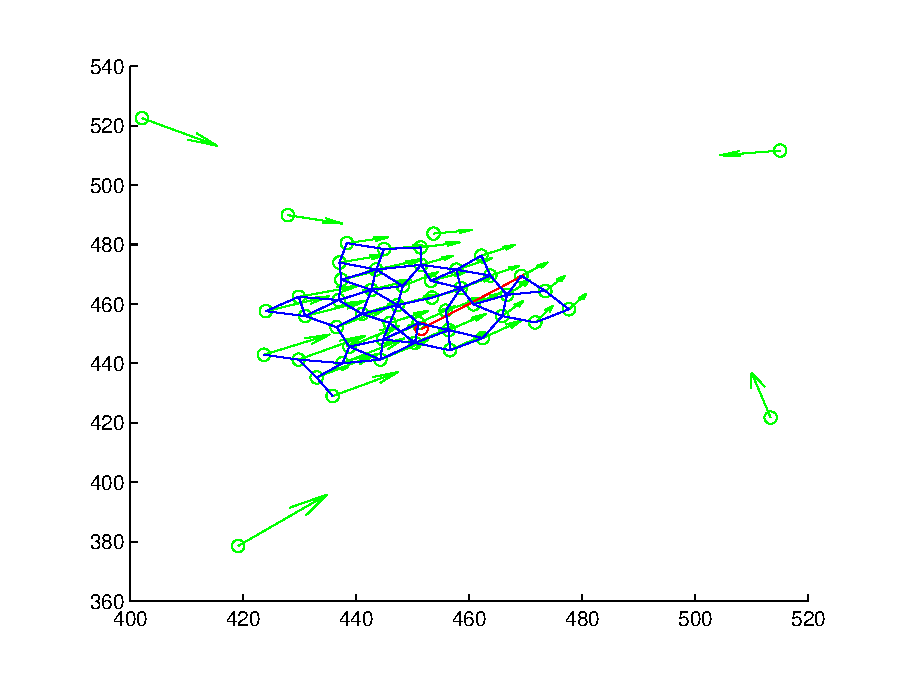
\includegraphics[width=3.45in]{n50m2vmax100amax1000t16delay}
  \end{center}

  \caption{\small N=50, m=2, Time=16s, Delayed}
  \label{fig:n50m2vmax100amax1000t16delay}
\end{figure}

\begin{figure}[!h]
  \begin{center}
    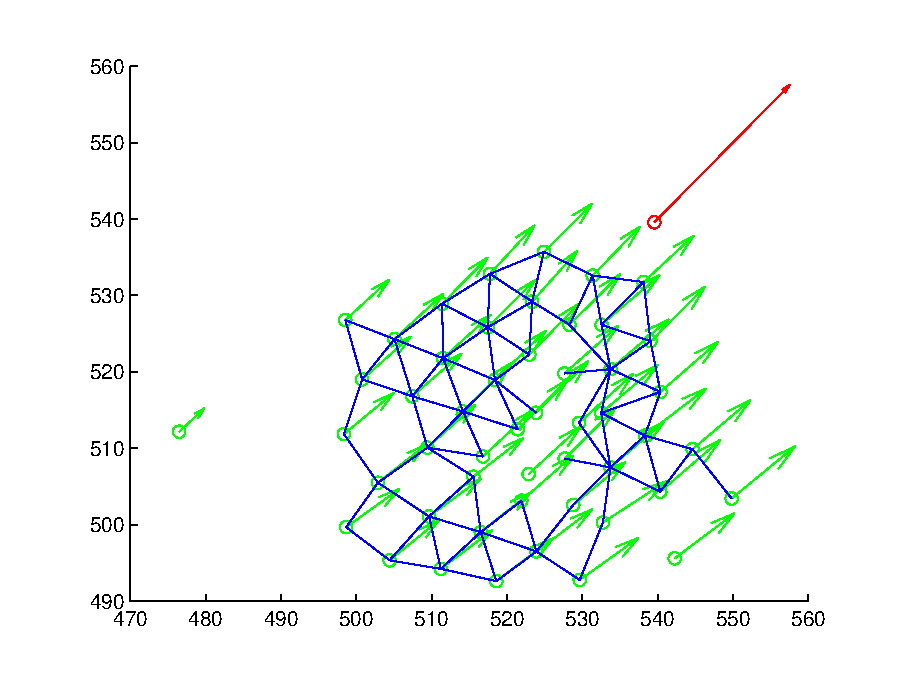
\includegraphics[width=3.45in]{n50m2vmax100amax1000t20delay}
  \end{center}

  \caption{\small N=50, m=2, Time=20s, Delayed}
  \label{fig:n50m2vmax100amax1000t20delay}
\end{figure}

\begin{figure}[!h]
  \begin{center}
    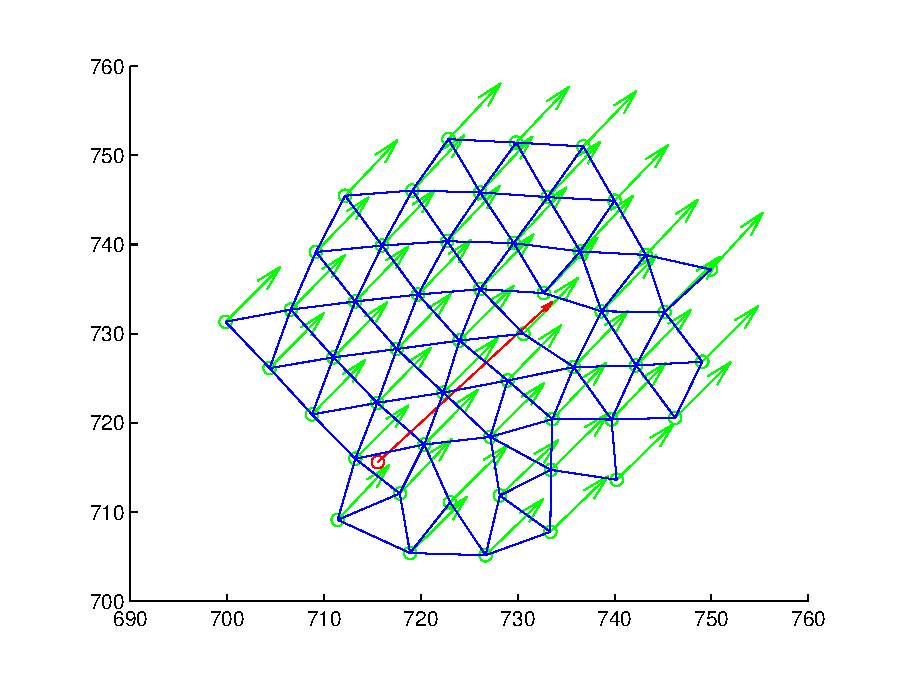
\includegraphics[width=3.45in]{n50m2vmax100amax1000t28delay}
  \end{center}

  \caption{\small N=50, m=2, Time=28s, Delayed}
  \label{fig:n50m2vmax100amax1000t28delay}
\end{figure}

\begin{figure}[!h]
  \begin{center}
    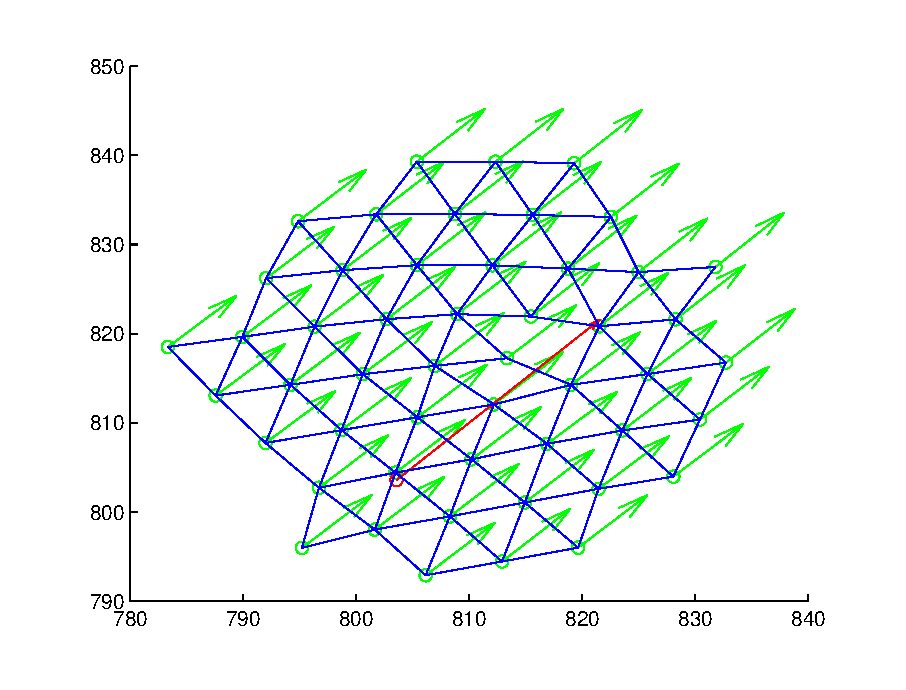
\includegraphics[width=3.45in]{n50m2vmax100amax1000t32delay}
  \end{center}

  \caption{\small N=50, m=2, Time=32s, Delayed}
  \label{fig:n50m2vmax100amax1000t32delay}
\end{figure}

\begin{figure}[!h]
  \begin{center}
    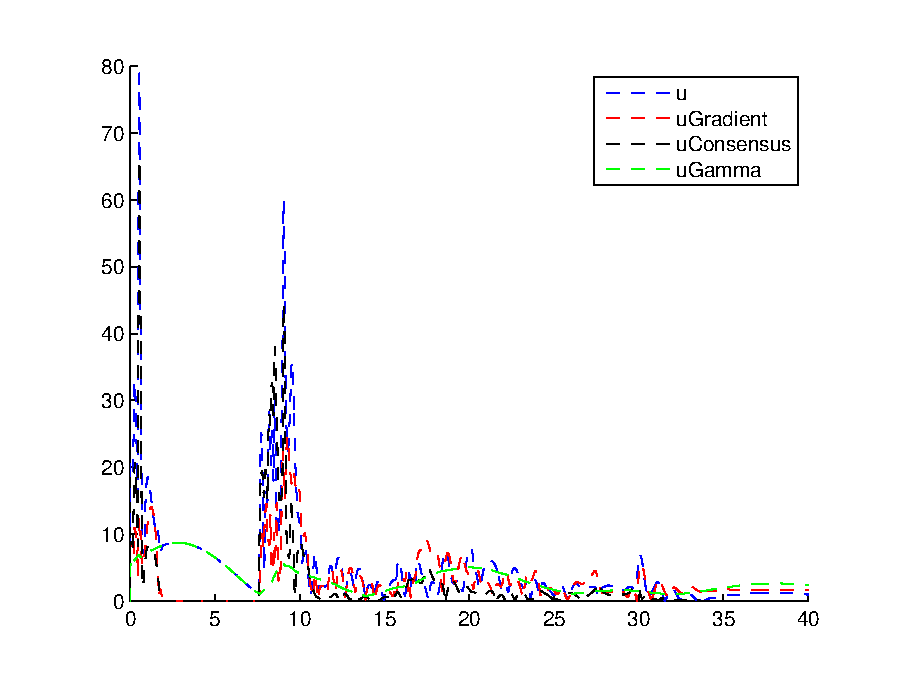
\includegraphics[width=3.45in]{n50m2vmax100amax1000delayControl}
  \end{center}

  \caption{\small N=50, m=2, Delayed, Control of One Node over Time}
  \label{fig:n50m2vmax100amax1000delayControl}
\end{figure}

\begin{figure}[!h]
  \begin{center}
    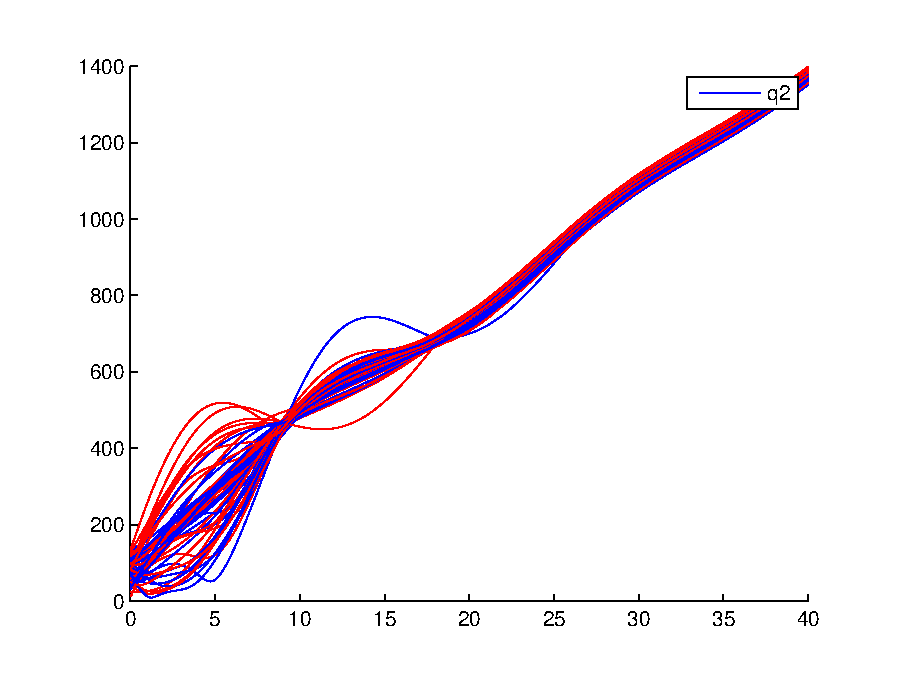
\includegraphics[width=3.45in]{n50m2vmax100amax1000delayPosition}
  \end{center}

  \caption{\small N=50, m=2, Delayed, Position of All Nodes over Time}
  \label{fig:n50m2vmax100amax1000delayPosition}
\end{figure}

\clearpage

\subsection{Combinations of Constraints}

Simulation with $v_{max}=100m/s$ and $a_{max}=100m/s^2$ can be seen in Figures~\ref{fig:n50m2vmax100amax100t00} to ~\ref{fig:n50m2vmax100amax100t32}, with the control in Figure~\ref{fig:n50m2vmax100amax100control}.

Finally, simulation with $v_{max}=100m/s$, $a_{max}=100m/s^2$, in the presence of delays and asynchronous control updates (each node updates at a different time with a different sampling time, $T_c$ in the range $0.1s$ to $0.2s$, using values of other nodes in the past, from $0.1s$ old to $0.2s$) can be seen in Figures~\ref{fig:n50m2vmax100amax10000t08delayAsync} to ~\ref{fig:n50m2vmax100amax10000t32delayAsync}, with a detail of the final time in \ref{fig:n50m2vmax100amax10000t32delayAsyncZoom}, with the control in Figure~\ref{fig:n50m2vmax100amax10000delayAsyncControl}, and the position of all nodes over time in Figure~\ref{fig:n50m2vmax100amax10000delayAsyncPosition}.

\begin{figure}[!h]
  \begin{center}
    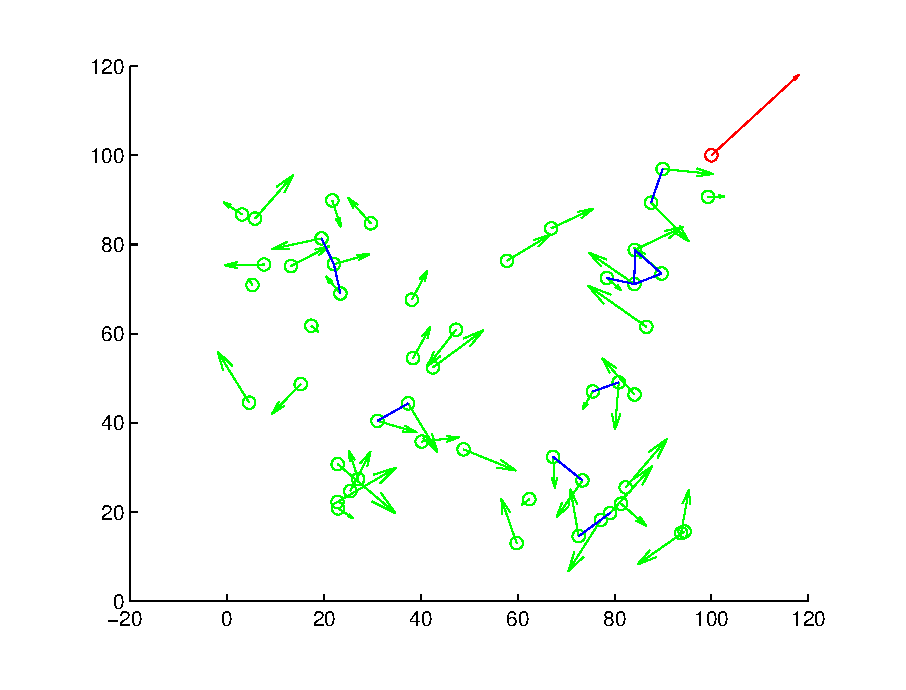
\includegraphics[width=3.45in]{n50m2vmax100amax100t00}
  \end{center}

  \caption{\small N=50, m=2, Time=0s, $v_{max}=100m/s$, $a_{max}=100m/s^2$}
  \label{fig:n50m2vmax100amax100t00}
\end{figure}

\begin{figure}[!h]
  \begin{center}
    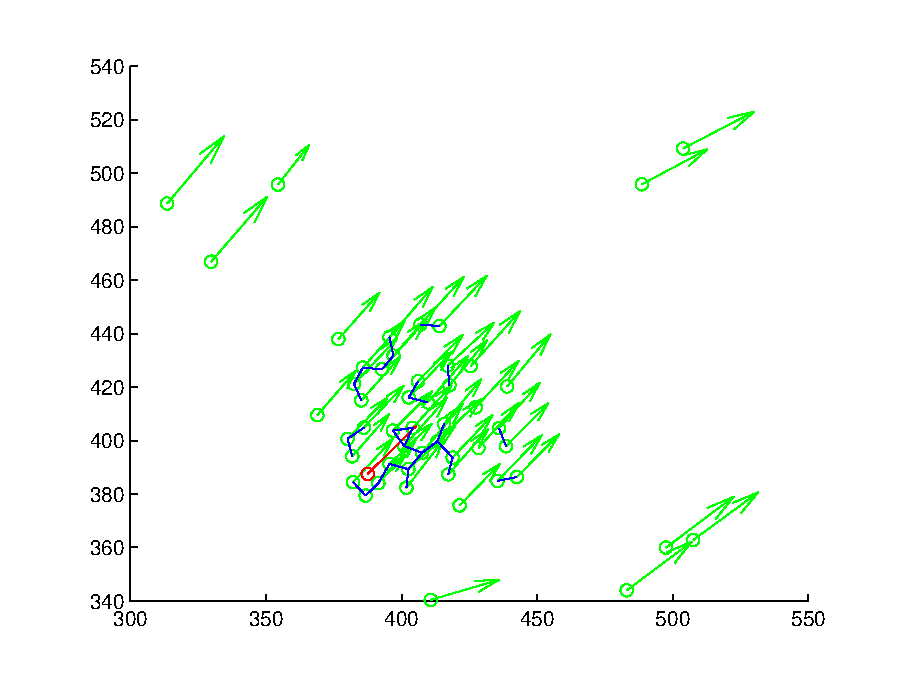
\includegraphics[width=3.45in]{n50m2vmax100amax100t12}
  \end{center}

  \caption{\small N=50, m=2, Time=12s, $v_{max}=100m/s$, $a_{max}=100m/s^2$}
  \label{fig:n50m2vmax100amax100t12}
\end{figure}

\begin{figure}[!h]
  \begin{center}
    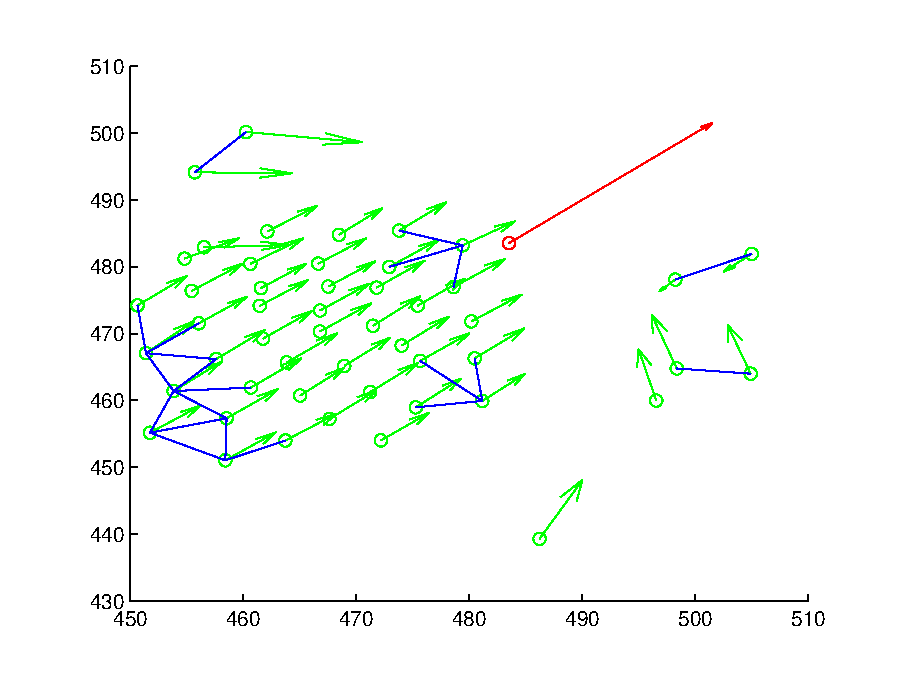
\includegraphics[width=3.45in]{n50m2vmax100amax100t16}
  \end{center}

  \caption{\small N=50, m=2, Time=16s, $v_{max}=100m/s$, $a_{max}=100m/s^2$}
  \label{fig:n50m2vmax100amax100t16}
\end{figure}

\begin{figure}[!h]
  \begin{center}
    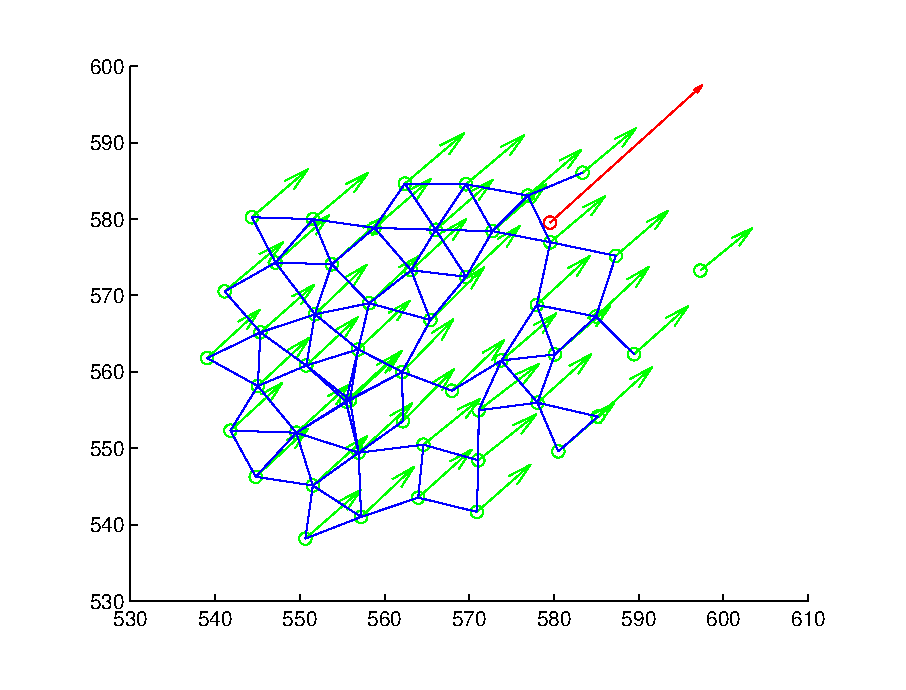
\includegraphics[width=3.45in]{n50m2vmax100amax100t20}
  \end{center}

  \caption{\small N=50, m=2, Time=20s, $v_{max}=100m/s$, $a_{max}=100m/s^2$}
  \label{fig:n50m2vmax100amax100t20}
\end{figure}

\clearpage

\begin{figure}[!p]
  \begin{center}
    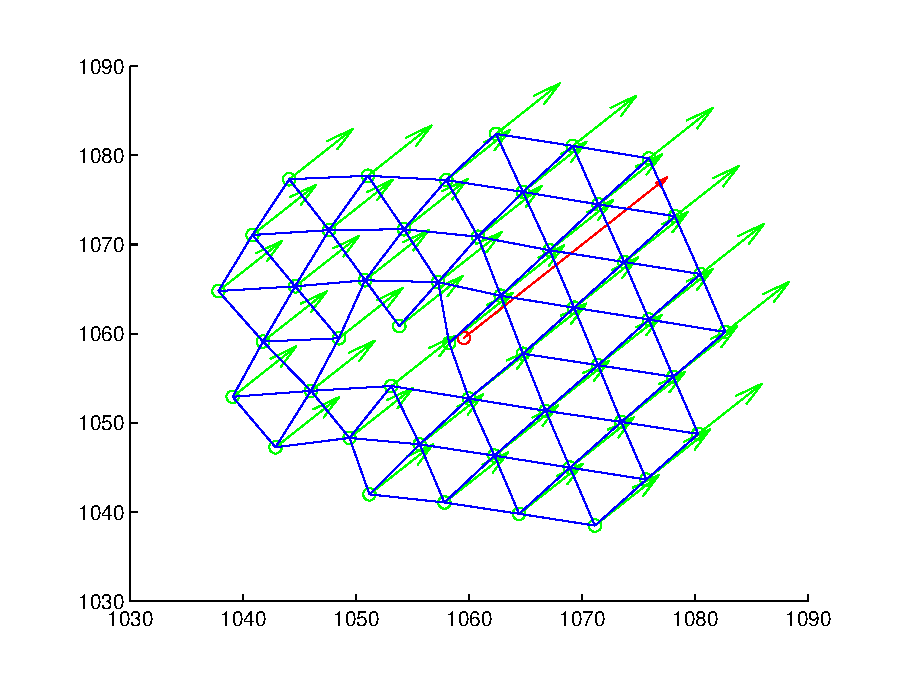
\includegraphics[width=3.45in]{n50m2vmax100amax100t32}
  \end{center}

  \caption{\small N=50, m=2, Time=32s, $v_{max}=100m/s$, $a_{max}=100m/s^2$}
  \label{fig:n50m2vmax100amax100t32}
\end{figure}

\begin{figure}[!p]
  \begin{center}
    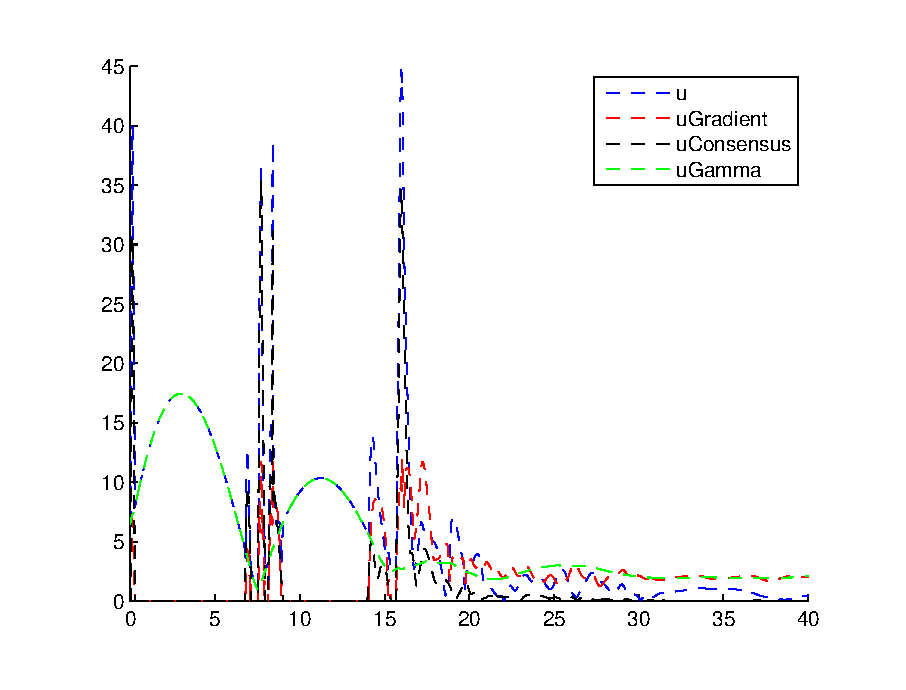
\includegraphics[width=3.45in]{n50m2vmax100amax100control}
  \end{center}

  \caption{\small N=50, m=2, Control Value of One Node over Time, $v_{max}=100m/s$, $a_{max}=100m/s^2$}
  \label{fig:n50m2vmax100amax100control}
\end{figure}

\begin{figure}[!p]
  \begin{center}
    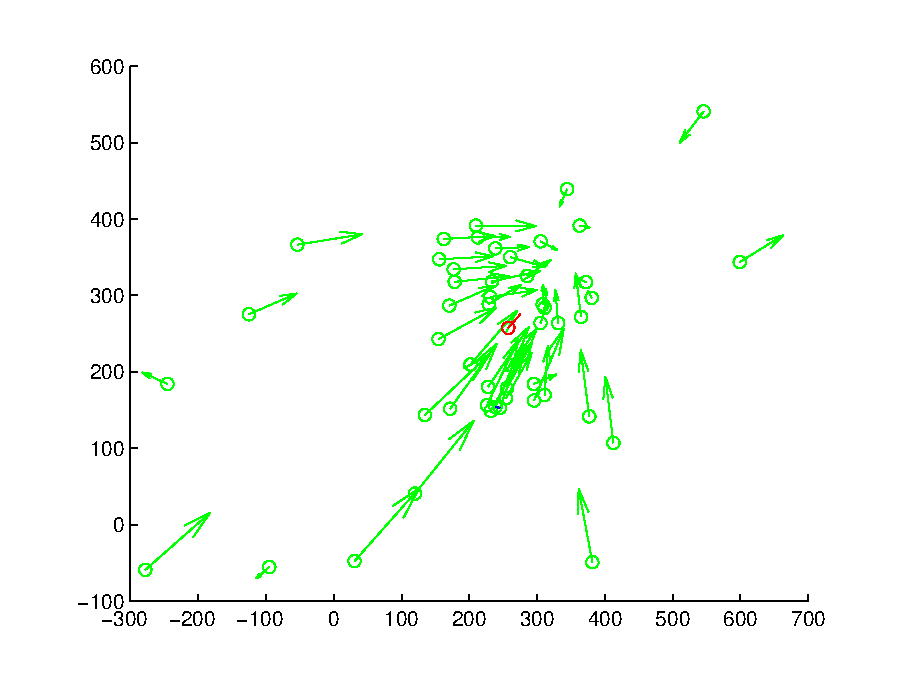
\includegraphics[width=3.45in]{n50m2vmax100amax10000t08delayAsync}
  \end{center}

  \caption{\small N=50, m=2, Time=8s, $v_{max}=100m/s$, $a_{max}=100m/s^2$, Delayed, Asynchronous}
  \label{fig:n50m2vmax100amax10000t08delayAsync}
\end{figure}

\begin{figure}[!p]
  \begin{center}
    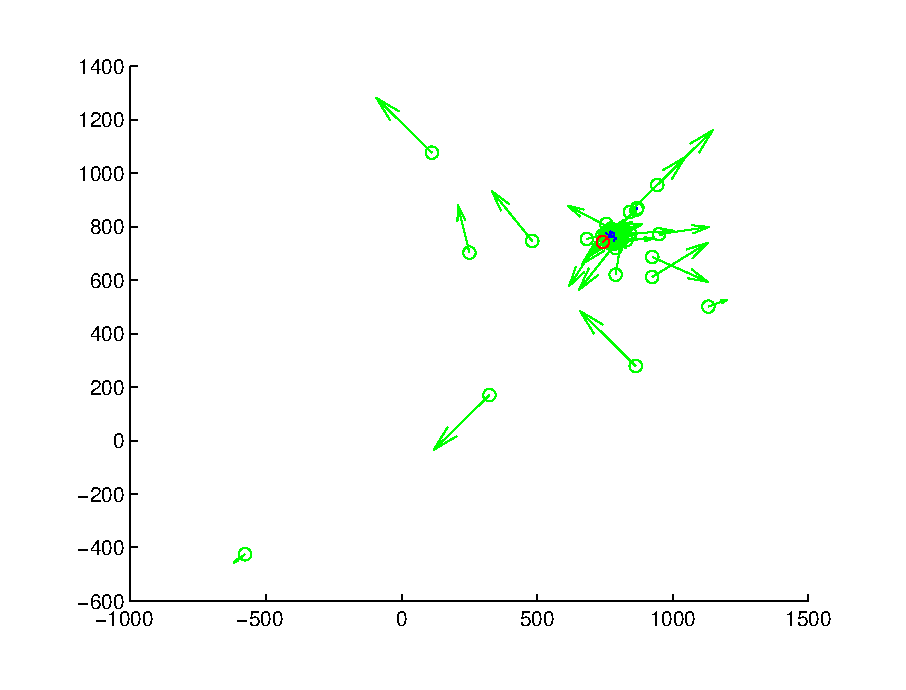
\includegraphics[width=3.45in]{n50m2vmax100amax10000t32delayAsync}
  \end{center}

  \caption{\small N=50, m=2, Time=32s, $v_{max}=100m/s$, $a_{max}=100m/s^2$, Delayed, Asynchronous}
  \label{fig:n50m2vmax100amax10000t32delayAsync}
\end{figure}

\clearpage

\begin{figure}[!p]
  \begin{center}
    \includegraphics[width=3.45in]{n50m2vmax100amax10000t32delayAsyncZoom}
  \end{center}

  \caption{\small N=50, m=2, Time=32s, $v_{max}=100m/s$, $a_{max}=100m/s^2$, Delayed, Asynchronous (Detail)}
  \label{fig:n50m2vmax100amax10000t32delayAsyncZoom}
\end{figure}

\begin{figure}[!p]
  \begin{center}
    \includegraphics[width=3.45in]{n50m2vmax100amax10000delayAsyncControl}
  \end{center}

  \caption{\small N=50, m=2, Control Value of One Node over Time, $v_{max}=100m/s$, $a_{max}=100m/s^2$, Delayed, Asynchronous}
  \label{fig:n50m2vmax100amax10000delayAsyncControl}
\end{figure}

\begin{figure}[!h]
  \begin{center}
    \includegraphics[width=3.45in]{n50m2vmax100amax10000delayAsyncPosition}
  \end{center}

  \caption{\small N=50, m=2, Position Values of All Nodes over Time, $v_{max}=100m/s$, $a_{max}=100m/s^2$, Delayed, Asynchronous}
  \label{fig:n50m2vmax100amax10000delayAsyncPosition}
\end{figure}

\clearpage

\section{Future Work}
\label{sec:future}
This work presented simulations of the effects that constraints that would be seen in real-world implementations of distributed control systems.
%
However, our understanding of real-world distributed control systems would be incomplete without understanding the effect of failures on such systems.
%
Computers and communication channels failures are captured by failure models from distributed computing such as crashes, omissions, and byzantine behavior, and their effect on computing systems have been well studied in the literature. 
%
In fact, the central theme in the distributed computing research is understanding the power and limitations of computing systems under different types of failures. 
%
Results in this area provide algorithms for solving canonical problems such as consensus, leader election, and clock synchronization in the presence of certain types of failures, and also establish lower bounds about impossibility of solving those problems with certain resource constraints.
%
Distributed control systems consist not only of computers, but also the physical world which they interact with through sensors and actuators. 
%
Thus, to understand the power and limitations of real-world distributed control systems, we are initiating the study of such systems in the face of computer, communications, sensor, and actuator---failures. 
%
This will require new failure models, as sensors and actuators require completely new failure models, whereas crash, slow, and byzantine failure mitigation must be modified to ensure properties in the physical world.
%
In addition, we need to consider new failure models for computers, such as timing failures. 
%
All of these failures now have physical manifestations, directly challenging safety of the control system.

In distributed computing, failure detection is often very hard, for example, one cannot tell differentiate between a slow and a crashed computer in an asynchronous system.
%
In contrast, failure detection is often easy for actuators, for instance, if an aileron on an airplane is stuck-at a value, a sensor as simple as a potentiometer could detect that it is not responding to control action as it is not changing position.
%
Timing failures can be analyzed offline through worst-case execution time (WCET) analysis, and also can be detected by runtime environment, such as in \cite{HenzingerGiotto2001}.
%
The prevalence of these classes of failures suggests new fault-tolerance strategies for distributed control systems.
%
The overall goal is to combine fault detection with the model for physical manifestation of failure to avoid bad states.

Toward this goal, we are studying the hybrid system modeled as hybrid input/output automata (HIOA) \cite{lynchSV2003}.  The HIOA of the physical world and flocking algorithm are shown in the hybrid input/output automata language \cite{mitra01masters} in Figure~\ref{fig:physicalWorld} and Figure~\ref{fig:agent_i}, respectively.

\begin{figure}[h!]
\centering
  \hrule
  {\lstinputlisting[language=ioa,firstline=1]{PhysicalWorld.hioa}}
  \hrule
  \caption{HIOA Model Physical World}
  \label{fig:physicalWorld}
\end{figure}

%
Informally, the system consists of $N$ agents starting at arbitrary locations on the real line, where $N \in \naturals, N > 1$ with the goal of 
\begin{inparaenum}[(a)]
\item reaching a fixed waypoint $x_g \in \reals$, and 
\item forming a {\em flock\/} or an equispaced formation on the way to $x^*$.
\end{inparaenum}  
The algorithm we shall study also works when a sequence of waypoints are presented to the agents, but for simplicity of presentation, we fix $x_g$.

The transition $send_i$ occurs at every time $\vx.now = next_i$ and adds a message containing physical state measurements of $\auto{Agent_i}$ to a $Queue$ in $\auto{PhysicalWorld}$ for each of $\auto{Agent_i}$'s communication neighbors, to be delivered before $\vx.now = d$, such that the state measurements are available for computation at $\vx.now = \vx.next_i$.  Also, the control for $\auto{Agent_i}$ is set at this transition, based on the measurement values at the time $\vx.now - \Delta$.
%
The transition $recv_{ij}$ removes a message containing physical state measurements of $\auto{Agent_j}$ from a $Queue$ in $\auto{PhysicalWorld}$ which is for $\auto{Agent_i}$ and adds it to a $\mathit{buffer}$.
%
Thus, each $\auto{Agent_i}$ receives knowledge of all nearby neighbors in time.

This state knowledge of neighbors is stored in a $\mathit{buffer}$ which maps from the set of indices of nodes, $[N]$ to $(\mathbb{R} \cup \{\perp\})^3$.  That is, if an $\auto{Agent_i}$ has not received a message from $\auto{Agent_j}$ yet, then $j \notin nbrs_i$, and thus the mapping with $j$ will yield triple of $\{\perp\}$s.
%
Each of the functions $\hat{x}$, $\hat{v}$, and $\hat{u}$ maps from the set of neighbors of $\auto{Agent_i}$, $nbrs_i$ to triples of physical state variables in $\math{R}$.  This achieves the same result as accessing the $\mathit{buffer}$, we should clarify this, as it should be the case that $\hat{x}(j)=\mathit{buffer}(j)=x_j$ from time $\vx.next_i - \Delta$.  We are using the $\mathit{buffer}$ behind the scenes to actually store the message values, and then just use the functions $\hat{x}$, $\hat{v}$, and $\hat{u}$ as a convenient notation.

\begin{figure}[h!]
\centering
  \hrule
  {\lstinputlisting[language=ioa,firstline=1]{Agent_i.hioa}}
  \hrule
  \caption{HIOA Model of $Agent_i$}
  \label{fig:agent_i}
\end{figure}

The control, $ctrl(i, x_g, x_i, v_i, u_i, \hat{x}, \hat{v}, \hat{u}, nbrs_i)$, is still being defined.
%
Let $\A$ be the HIOA obtained by composing $\auto{PhysicalWorld} \| \auto{Agent}_1 \| \ldots \auto{Agent}_N$.  We denote a state of $\A$ by $\vx$ and individual state components by $\vx.x_i$, $\vx.\mathit{next}_i$, etc.
%

We would like to show that the \textit{safety property}, that the distance between each node $i$ and $j$ is at least $\mathit{r_{safety}}$ is satisfied.  Assume that the network delay between nodes is bounded, such that a message sent by node $i$ is received by all its communication neighbors within time $d$.  This assumption immediately gives that all $recv_{ij}$ and $recv_{ji}$ actions will be correct, in that the necessary state information is delivered before the next period.

\begin{inv}
$\I_{safety}\left(S\right) = \\
	\left\{ \begin{array}{l}
		\textrm{if } \left( \vx.now = \vx.next_i \right) \wedge \neg \vx.Send \Rightarrow \\
		\forall i \left(\vx.x_{i} - \vx.x_{i-1}\right) + \Delta\left(\vx.v_{i} - \vx.v_{i-1}\right) + \frac{1}{2}a_{max}\Delta^2 \geq \\ \mathit{r_{safety}} \\
		\textrm{if } \left( \vx.now \neq \vx.next_i \right) \vee \left( \vx.now = \vx.next_i \wedge Send \right) \Rightarrow \\
		\forall i \left(\vx.x_{i} - \vx.x_{i-1}\right) + t_{Rem}\left(\vx.v_{i} - \vx.v_{i-1}\right) + \frac{1}{2}a_{max}t_{Rem}^2 \geq \\  \mathit{r_{safety}} \\
	\end{array}
\right.$ where $t_{Rem} \equiv \left(\vx.next_i - \vx.now\right)$.
\end{inv}

We are working on a proof of this presently and eventually would like to consider the same proof with faults also in the system.

\section{Conclusions}
\label{sec:conclusion}

This paper presented simulation results arising from the implementation of the flocking problem formalized in Olfati-Saber's paper \cite{os2006}.
%
Without constraints, the system reached the goal state and formed a flock (see Figure~\ref{fig:n50m2t32}.
%
With only velocity constraints, the system easily reached the goal state and formed a flock, as the actuator magnitude easily compensated for any velocity and position problems, although due to the limitation in velocity, it would take a very long time for the system to globally achieve this result (see Figure~\ref{fig:n50m2vmax1t32}.
%
Not surprisingly, in the face of actuator constraints, it was not always possible to achieve either of the objectives, that of forming a flock and reaching the goal, as the saturated control value was not enough to overcome the initial velocities, so the system actually globally diverges (see Figure~\ref{fig:n50m2vmax1000amax1t32}.
%
When considering delay with reasonable state and actuator constraints, the system achieved the desired goals as well (see Figure~\ref{fig:n50m2vmax100amax1000t32delay}.
%
With equal actuator and velocity constraints, the system achieved the desired goals (see Figure~\ref{fig:n50m2vmax100amax100t32}).
%
However, when considering both delay and asynchronous control updates with reasonable actuator and state constraints, the system did not globally achieve the objectives (see Figure~\ref{fig:n50m2vmax100amax10000t32delayAsync}), although subsets of it (see Figure~\ref{fig:n50m2vmax100amax10000t32delayAsyncZoom}).



\label{sec:references}
\bibliographystyle{IEEEtran}
\bibliography{IEEEabrv,flocking}




















%
%First, consider a model of communication where all agents synchronously send messages to all other nodes within a communication radius $r_{comm}$ of their current position every $\Delta$ time.  The set of nodes within the communication radius of a node $i$ is called the \textit{communication neighbors} of $i$ and is defined as $N_c(i) = N(i, r_{comm}) \equiv \left\{ j \in [N] : \abs{x_i - x_j} \leq r_{comm}\right\}$.  Also at every $\Delta$ time, each node $i$ updates its own control law, $u_i$.  This scenario is that every node $i$ is updating its control $u_i$ using the states of all of its neighbors from time $start = next - \Delta$.
%
%%That is, all nodes $i$ and $j$ communicate at $now \geq k*\Delta$ where $k \in \mathbb{N}$ and $j : \forall i . \abs{x_{i} - x_{j}} \leq r_{comm}$.
%
%We assume the following of $S_0$:
%
%$ \begin{array}{ll}
%		1) & x_i > 0 \\
%		2) & \textrm{ if } j > i \Rightarrow x_j > x_i \\
%		3) & \abs{v_i - v_{j}} < 2v_{max} \\
%		4) & \abs{x_i - x_{j}} > r_{init} \\
%		5) & u_i = 0 \\
%		6) & x_g > x_i
%	\end{array} $
%$\forall i, j \in N$ and $i \neq j$.
%
%Communications radius: $r_{comm}$
%
%Safety radius: $\mathit{r_{safety}}$
%
%Initial radius to maintain safety: $r_{init}$
%
%$r_{comm} > r_{init} > \mathit{r_{safety}}$
%
%The control, $ctrl(i, x_g, x_i, v_i, u_i, \hat{x}, \hat{v}, \hat{u}, nbrs_i)$, is defined as
%
%$ctrl\left(i, x_g, x_i, v_i, u_i, \hat{x}, \hat{v}, \hat{u}, nbrs_i \right) = \\
%	\left\{
%		\begin{array}{ll}
%			\sgn{x_g - x_i}a_{max} & \textrm{if } nbrs_i = \{\} \\
%				\left\{
%					\begin{array}{l}
%						\sgn{\tilde{v}}a_{max} \textrm{  if } \abs{x_i - \tilde{x}} \leq r_{init} \\
%						a\left(\tilde{x} - x_i\right - r_{init}) + b\left(\tilde{v} - v_i\right) \textrm{  else }
%					\end{array}
%				\right.
%			& \textrm{ else} \\
%		\end{array}
%	\right. $
%
%where $\tilde{x} = \hat{x}(\tilde{i})$, $\tilde{v} = \hat{v}(\tilde{i})$, $\tilde{u} = \hat{u}(\tilde{i})$, $\tilde{i} = \argmin{\left(\hat{x}(j) - x_i\right)}{j \in nbrs_i}$, $a \in \mathbb{R}_+$, and $b \in \mathbb{R}_+$.
%
%We would like to show that the \textit{safety property}, that the distance between each node $i$ and $j$ is at least $\mathit{r_{safety}}$ is satisfied.  However, before we begin working toward the safety property, we must make some assumptions about communications and prove some simpler invariants.  First, assume that the network delay between nodes is bounded, such that a message sent by node $i$ is received by all its communication neighbors $j \in N_c(i)$ within time $d$.  This assumption immediately gives that all $recv_{ij}$ and $recv_{ji}$ actions will be correct, in that the necessary state information is delivered before the next period.
%
%
%%
%%Notes: while of course no nodes have knowledge of all of $S$ for the actual operation, for the proof we can assume we have all of this knowledge.  Basically, as long as all nodes start far enough apart, with bounded relative velocities, and a fast enough update period $\Delta$, we can guarantee that all nodes receive messages between $\Delta$.
%
%Recall from above that $d < \Delta$, that is, the \textit{communications delay} $d$ is such that messages are delivered before control updates that occur at $\Delta$.
%
%\textbf{Invariant}
%
%$\forall i, j, agent_i.now_i = agent_j.now_j = PhysicalWorld.now$
%
%This is given by the assumption of synchronous communication.
%
%\textbf{Invariant}
%
%All nodes receive messages about the state information from time $next - \Delta$ before time $next$.
%
%Define the time for the last send with respect to state $s$ as $start(s) = s.next - \Delta$.
%
%$s.nbrs_i = N(i, r_{comm})(start(s))$
%
%$\I_{nbrs}\left(S\right) = \\
%	\left\{
%		\begin{array}{l}
%			\textrm{if } s.now - start(s) \geq d \textrm{ then } s.nbrs_i = N_c(i)(start(s))\\
%			\textrm{elseif } s.now - start(s) < d \textrm{ then } N_c(i)(start(s)) = s.nbrs_i \cup \{s.Channel_{ij}\}\\
%		\end{array}
%	\right.$
%
%Fix a reachable state $s$.  Expanding $s.now - start(s) \geq d$ to $s.now - s.next + \Delta \geq d$, it is clear that if $s.now \geq start(s) + d$, all messages will have been delivered due to the stopping condition for the $recv_{ij}$ actions to occur in $PhysicalWorld$.  However, before that time in the other case, all messages may still be in the channel since no stopping condition has been reached (and all messages were put in the channel at time $start(s)$), or some messages may have been delivered already, so all messages are either in the channel or have been delivered, and thus, the set of neighbors of node $i$ is the union of these.  All closed trajectories $\tau$ that could violate this are excluded by the stopping condition.
%
%\textbf{Invariant}
%
%The set of \textit{communication neighbors} of node $i$ at time $next - \Delta$ is the same as the set of \textit{physical neighbors} at time $start + d$.
%
%\textbf{Invariant}
%
%$\I_{channelSize}\left(S\right) = \textrm{if } \Delta > d \textrm{, then } size(Channel_{ij}) \leq 1$
%
%This holds trivially since all messages will be delivered by time $now + d$, so they will be inserted and removed from the queue in $PhysicalWorld$ before the next $\Delta$.
%
%Slightly more formally (should be stated in this manner as the invariant?):
%
%Size when $now = start$ is 1, since all messages are in the channel after the $Send_i$ action occurs at time $start$.
%
%Size between $now = start$ and $now = start + d$ is either 0 or 1, since some messages may have been delivered, but some may not have.
%
%Size between $now = start + d$ and $\Delta$ is 0, since all messages must have been delivered by the stopping conditions and thus no closed trajectory $\tau$ could have crossed this boundary.
%
%\textbf{Invariant}
%
%If $r_{comm} > r_{init}$, then nodes within at least $r_{comm}$ of one another get messages before their distance is less than $r_{init}$.  Nodes may then be within between $r_{init}$ and $\mathit{r_{safety}}$ of one another.
%
%Denote the time required to change a node's velocity from maximum to minimum (and vice-versa) as $t_a = \frac{2v_{max}}{a_{max}}$.  Denote the time required to travel between the communication radius and the safety radius as $t_v = \frac{r_{comm} - \mathit{r_{safety}}}{2v_{max}}$.  Then, $\Delta = \min(t_a, t_v)$.
%
%Denote the distance covered while changing a node's velocity from one extrema to the other as $r_a = 2v_{max}t_a = \frac{4v_{max}^2}{a_{max}}$.  Denote the maximum distance traveled during the delay as $r_d = 2v_{max}\Delta$.
%
%Note that we must fix one of $r_{comm}$ or $\Delta$, as they are functions of one another.  We can then ensure the given $r_{comm}$ and computed $\Delta$ (or vice-versa) satisfy the initial conditions.
%
%\textbf{Invariant}
%
%Assume $S_0$ is given such that $\I_{recv}(S_0)$ is satisfied at time $t_0$, then $\I_{recv}(S)$ is satisfied, and thus the receive property is maintained $\forall t \geq t_0$.
%
%We are given that $S_0$ is such that at the initial time $t_0$ the invariant $\I_{recv}(S_0)$ is satisfied.  This gives us the following
%
%$\forall S \xrightarrow{a} S^{\prime} : \I_{recv}\left(S\right) \Rightarrow \I_{recv}\left(S^{\prime}\right)$
%
%We consider each action separately in cases:
%
%i) $Send$
%
%ii) $Recv$
%If the delay $d$ between messages is less than the period of synchronous communication $\Delta$, then all $Recv$ actions will have occurred before the next period.
%
%$\forall \tau,\textrm{ if } \forall S \xrightarrow{\tau} S^{\prime} : \I_{recv}\left(S\right) \Rightarrow \I_{recv}\left(S^{\prime}\right)$
%
%While it is tempting to say that the worst scenario for $Recv$ is when two neighbors $i$ and $j$ are moving away from one another with maximum velocity and acceleration, this is actually not the case if we only care about the safety property defined as no nodes come within $\mathit{r_{safety}}$ of one another.  The worst case is still when these two nodes are coming together with maximum acceleration and velocity, and that they are \textbf{not} yet within $r_{comm}$.  If they can cover their distance $\abs{x_i - x_j}$ before the next $\Delta$, plus some details on the velocity and number of cycles required to change direction, then they may collide.  What we want is an upper bound of $\Delta$ to guarantee everything, such as the following:
%
%%$\Delta(x, v) \equiv \frac{x_i - x_j - r_{comm}}{v_i - v_j}$
%%
%%or, with acceleration:
%%
%%$\Delta(x, v) \equiv \frac{x_i - x_j - r_{comm}}{v_i - v_j} - \frac{v_i - v_j}{a_{max}}$
%%
%%and with existing bounds:
%%
%%$\Delta(x, v) \equiv \frac{\mathit{r_{safety}} - r_{comm}}{C_1} - \frac{C_1}{a_{max}}$
%%
%%(or equivalently:)
%%
%%$\Delta(x, v) \equiv \frac{\mathit{r_{safety}} - r_{comm}}{2v_{max}} - \frac{2v_{max}}{a_{max}}$
%%
%%The above seems a bit wrong, the following seems correct:
%%
%%$\Delta(x, v) \equiv \frac{C_1 - \frac{r_{comm}}{\Delta}}{a_{max}}$
%%
%%or equivalently: $\Delta(x, v) \equiv \frac{2v_{max} - \frac{r_{comm}}{\Delta}}{a_{max}}$
%%
%%where we replace $\Delta$ with $t_{Rem}$
%%
%%$\Delta(x, v) \equiv \frac{C_1 - \frac{r_{comm}}{t_{Rem}}}{a_{max}}$
%
%Note that we really should not have to talk about $u_i > 0$ as different to the $a_{max}$ case, since the worst affect on $\mathit{r_{safety}}$ comes from $v_i$, which if bounded by $v_{max}$ is already done.  Any time we have acceleration and the particles are moving at less than $v_{max}$, as long as we know we work for $v_{max}$, we will work for anything less than $v_{max}$, regardless of the rate of change of $v_i$.
%
%However, when two nodes are moving away from one another with maximum acceleration and velocity is the worst case for flocking.  If we enforce an initial condition about all nodes being within $r_{comm}$, and that their initial velocities are not such that they can leave $r_{comm}$ before the first control update, then we should be able to guarantee flocking for all time.  This gives us both an upper and lower bound on $r_{comm}$.  (Note: We should check to see if this definition on initial conditions is basically what Olfati-Saber is referring to in the previous work for Algorithm 1 to maintain flocking instead of segmentation.)
%
%%Consider two particles $i$ and $j$ that are going towards one another with maximum acceleration (and $x_j > x_i$, that is, $j$ is to the right of $i$) that are not yet communication neighbors (that is, $\abs{x_i - x_j} > r_{comm}$), such that from time $t$ (or $k*\Delta$), where the control was applied, and time $t+\Delta$ (or $(k+1)*\Delta$).
%%
%%We want first to show: If $\abs{x_i(t) - x_j(t)} > r_{comm}$, then $\abs{x_i(t) - x_j(t)} \geq \mathit{r_{safety}}$
%%
%%$x_i(t+\Delta) = x_i(t) + v_i(t)\Delta + \frac{1}{2}a_{max}\Delta^2$
%%
%%$x_j(t+\Delta) = x_j(t) - v_j(t)\Delta - \frac{1}{2}a_{max}\Delta^2$
%%
%%$x_i(t+\Delta) - x_j(t+\Delta)$
%%
%%$x_i(t) + v_i(t)\Delta + \frac{1}{2}a_{max}\Delta^2 - (x_j(t) - v_j(t)\Delta - \frac{1}{2}a_{max}\Delta^2) \geq \mathit{r_{safety}}$
%%
%%$x_i(t) - x_j(t) + (v_i(t) + v_j(t))\Delta + a_{max}\Delta^2$
%%
%%$x_i(t) - x_j(t) + 2(v_{max})\Delta + a_{max}\Delta^2$
%
%%\textbf{Invariant}
%%
%%Controls decrease relative velocities of nodes coming towards one another.  If two nodes are coming together at step $x$, then at step $x^\prime$, their relative velocities must have decreased.  This gives us one bound for the periodicity: $\Delta \leq \frac{\overline{v_{rel}}}{a_{max}}$.  The other bound comes from $\Delta \leq \frac{\mathit{r_{safety}}}{\overline{v_{rel}}}$.  This lets us define $\Delta = \min{\frac{\overline{v_{rel}}}{a_{max}}, \frac{\mathit{r_{safety}}}{\overline{v_{rel}}}$.  This follows from Invariant 3 and the definition of the control.
%%
%%If at $k$, $\abs{v_i - v_j} = c$, then at $k+1$, $\abs{v_i - v_j} < c$.
%%
%%send: no affect on this node's state
%%recv: does affect control: must show that values arrive in $\Delta$, such that values for $x^\prime$ are from $x$.
%%$\tau$: know values at $x^\prime$ are from $x$, so we applied the appropriate control to avoid collision (reduced velocity): does this imply the control needs to use $r_{init}$ instead of $\mathit{r_{safety}}$ for the part where it switches the direction of control?
%%
%%At any rate, since $\exists \overline{v_{rel}}$, then as long as $\mathit{r_{safety}} \leq \abs{x_i - x_j} + \overline{v_{rel}}\Delta$, then we are done.  The other absolute case, when $\abs{v_i - v_j} < \overline{v_{rel}}$, then we must have that $\mathit{r_{safety}} \leq \abs{x_i - x_j} + \abs{v_i - v_j}\Delta + a_{max}\Delta^2$.  The interim case, when neither we have maximum velocity nor acceleration is interesting, but is easily bounded by these others, and requires $\mathit{r_{safety}} \leq \abs{x_i - x_j} + \abs{v_i - v_j}\Delta + \abs{u_i - u_j}\Delta^2$.  The $\abs{u_i - u_j}$ is fixed to a constant value $u_c$ at the beginning of the period.  We can then make the claim that at most the relative velocity of $i$ and $j$ becomes $\overline{v_{rel}}$, so we are covered by the earlier case.
%
%\textbf{Invariant: No Reordering}
%
%$x_i < x_j \forall i < j$
%
%Base case: satisfied by assumption that $x_i < x_j$.
%
%Inductive case: bring in control from safety argument below
%
%
%
%\textbf{Invariant: Safety}
%
%Consider the safety invariant:
%
%$\I_{safety}\left(S\right) = 
%	\left\{ \begin{array}{l}
%		\textrm{if } \left( now = next \right) \wedge \neg Send \Rightarrow \\
%		\forall i \left(x_{i} - x_{i-1}\right) + \Delta\left(v_{i} - v_{i-1}\right) + \frac{1}{2}a_{max}\Delta^2 \geq \\ \mathit{r_{safety}} \\
%		\textrm{if } \left( now \neq next \right) \vee \left( now = next \wedge Send \right) \Rightarrow \\
%		\forall i \left(x_{i} - x_{i-1}\right) + t_{Rem}\left(v_{i} - v_{i-1}\right) + \frac{1}{2}a_{max}t_{Rem}^2 \geq \\  \mathit{r_{safety}} \\
%	\end{array}
%\right.$ where $t_{Rem} \equiv next - now$.
%
%There are three possible cases that can arise for the controls at $next$, assuming at $start$ the state is okay:
%
%1) There are two interesting cases, both are when nodes can now communicate when they could not before.  First, when nodes are still more than $r_{init}$ apart, they apply
%
%$r_{comm} \geq \abs{x_i - x_j} \geq r_{init} > \mathit{r_{safety}}$
%
%$u_i = a\left(\tilde{x} - x_i\right - r_{init}) + b\left(\tilde{v} - v_i\right)$
%
%2) Second, when nodes are less than $r_{init}$ apart, they apply the collision avoidance control
%
%$r_{comm} \geq r_{init} > \abs{x_i - x_j} > \mathit{r_{safety}}$
%
%$u_i = \sgn{v_j}a_{max}$
%
%The only time this situation arises (as in, this is the only time we can recover from it) is as follows:
%
%$r_{comm} \geq r_{init} > \abs{x_i - x_j} > r_{init} - r_d > \mathit{r_{safety}}$
%
%that is, the nodes must still be separated by the radius required to recover safety, but can tolerate the distance covered over the delay.
%
%3) The most boring case is when nodes are still not communications neighbors, they just go towards the goal:
%
%$\abs{x_i - x_j} > r_{comm} > r_{init} > \mathit{r_{safety}}$
%
%$u_i = \sgn{x_g - x_i}*a_{max}$
%
%Discussion:  For the second invariant assumption, it is necessary to include the term $\left( now = next \wedge Send \right)$ as otherwise a single point at the $Send$ may be omitted.  Similarly, it is necessary to consider this condition for trajectories that are less than the length of $\Delta$.
%
%Assume $S_0$ is given such that $\I_{safety}(S_0)$ is satisfied.  If $\I_{safety}(S_0)$ is satisfied, then $\I_{safety}(S)$ is satisfied, and thus the safety property is maintained.
%
%We are given that $S_0$ is such that at the initial time $0$ the invariant $\I_{safety}(S_0)$ is satisfied.  This gives us the following
%
%$\forall S \xrightarrow{a} S^{\prime} : \I\left(S\right) \Rightarrow \I\left(S^{\prime}\right)$
%
%We consider each action separately in cases:
%i) $Send$
%Send does not affect the state of node $j$, and it does not affect the state of node $i$ until $next$, so it is vacuously true in both cases.
%
%ii) $Recv$
%Trivially from the $I_{recv}$ invariant.
%
%$\forall \tau, if \forall S \xrightarrow{\tau} S^{\prime} : \I\left(S\right) \Rightarrow \I\left(S^{\prime}\right)$
%
%For the trajectories, it is sufficient to consider the worst possible trajectory affecting the safety condition, that is, when particles are coming towards one another with maximum acceleration.  Given the assumption that $\abs{x_i - x_j} < C_1$, we see that the relative velocities of any particles are bounded, and we will be immediately finished.
%
%%Consider two particles $i$ and $j$ that are going towards one another with maximum acceleration (and $x_j > x_i$, that is, $j$ is to the right of $i$), such that from time $t$, where the control was applied, and time $t+\Delta$, the final positions will be determined by:
%%
%%If $\abs{x_i(t) - x_j(t)} \geq \mathit{r_{safety}}$, then 
%%
%%$x_i(t+\Delta) = x_i(t) + v_i(t)\Delta + \frac{1}{2}a_{max}\Delta^2$
%%
%%$x_j(t+\Delta) = x_j(t) - v_j(t)\Delta - \frac{1}{2}a_{max}\Delta^2$
%%
%%Want: $\abs{x_i(t+\Delta) - x_j(t+\Delta)} \geq r_{safety1}$
%%
%%$x_i(t) + v_i(t)\Delta + \frac{1}{2}a_{max}\Delta^2 - (x_j(t) - v_j(t)\Delta - \frac{1}{2}a_{max}\Delta^2) \geq r_{safety1}$
%%
%%$x_i(t) - x_j(t) + (v_i(t) + v_j(t))\Delta + a_{max}\Delta^2 \geq r_{safety1}$
%%
%%$x_i(t) - x_j(t) + (v_i(t) + v_j(t))\Delta + a_{max}\Delta^2 \geq r_{safety1}$
%%
%%To ensure we can handle this case, we really need that $r_{safety1}$ is at least this size:
%%
%%$x_i(t) - x_j(t) + 2(v_{max})\Delta + a_{max}\Delta^2 \geq r_{safety1}$
%%
%%$\mathit{r_{safety}} + 2(v_{max})\Delta + a_{max}\Delta^2 \geq r_{safety1}$
%%
%%This $r_{safety1}$ is the real bound for the starting states that we need to work with to easily ensure the invariant inductively.  We can also replace the $2v_{max}$ by $C_1$, the maximum relative velocities.
%
%In reality, given a large enough $r_{comm}$ (or small enough $\Delta$), this is overly conservative, as the control law would prohibit nodes from moving towards one another with acceleration $a_{max}$.
%
%
%\textbf{Invariant: Progress}
%
%Show that if $x_g > x_i$, then $v_i > 0 \forall i$ eventually and for long enough time to reach goal.  Symmetrically, if $x_g < x_i$, then $v_i < 0 \forall i$ eventually and for long enough time to reach goal.  That is, we must show that $\exists t_g$ such that $v_i t_g \geq x_g \forall i$.  (Slightly more complicated than this, integral of velocity over time?)
%
%Is it useful to do this proof as a stability proof, showing that eventually, $\forall i, v_i = v_max$, in the direction of the goal?
%
%Or equivalently, showing that $x_i - x_g = 0$, to say that the node eventually reaches the goal by stability.



\end{document}
